\documentclass{article}%tạo một bản báo cáo
% \documentclass[xcolor=table]{beamer}
\usepackage[utf8]{inputenc}
\usepackage[T5]{fontenc} % để sử dụng tiếng việt
\usepackage[fontsize=13pt]{scrextend} % set fontsize =13pt
\usepackage[paperheight=29.7cm,paperwidth=21cm,right=2cm,left=3cm,top=2cm,bottom=2.5cm]{geometry} % chuẩn A4, căn lề trái phải trên dưới
% \usepackage[paperheight=29.7cm,paperwidth=21cm,right=2cm,left=3cm,top=2cm,bottom=2.5cm,twoside]{geometry}% Chuẩn A4, căn lề phải, trái, trên, dưới.
\usepackage{mathptmx} %timenewRoman
\usepackage{graphicx} % thư viện chèn ảnh 
\usepackage{float} % set vị trí chèn ảnh 
\usepackage{tikz} % thư viện tạo khung bìa
\usepackage{enumerate}
\usepackage{changepage}
\usepackage{amsmath}
\usepackage{xltabular}
\usepackage{setspace}
\usepackage{pdfpages}
\usepackage{multirow}
% \usepackage{graphicx}
% \usepackage[table,xcdraw]{xcolor}

\usetikzlibrary{calc} % thư viện tikz
\usepackage{indentfirst} % thư viện thụt đầu dòng
\renewcommand{\baselinestretch}{1.2} % giãn dòng 1.2
\setlength{\parskip}{6pt} % giãn dòng giữa các đoạn văn(spacing after)
\setlength{\parindent}{1cm} % set khoảng cách thụt đầu dòng mỗi đoạn
\usepackage{titlesec} % thư viện để set up các kiểu  chữ
\setcounter{secnumdepth}{4}
\titlespacing*{\section}{0pt}{0pt}{30pt} % Heading 1
\titleformat*{\section}{\fontsize{16pt}{0pt}\selectfont \bfseries \centering}

\titlespacing*{\subsection}{0pt}{10pt}{0pt} % Heading 2
\titleformat*{\subsection}{\fontsize{14pt}{0pt}\selectfont \bfseries}

\titlespacing*{\subsection}{0pt}{10pt}{0pt} % Heading 3
\titleformat*{\subsection}{\fontsize{13pt}{0pt}\selectfont \bfseries \itshape}

\titlespacing*{\paragraph}{0pt}{10pt}{0pt} % Heading 4
\titleformat*{\paragraph}{\fontsize{13pt}{0pt}\selectfont \itshape}

\renewcommand{\figurename}{\fontsize{12pt}{0pt}\selectfont \bfseries Hình} %hình
\renewcommand{\thefigure}{\thesection.\arabic{figure}}
\usepackage{caption}
\captionsetup[figure]{labelsep=space}

\renewcommand{\tablename}{\fontsize{12pt}{0pt}\selectfont \bfseries Bảng} %bảng
\renewcommand{\thetable}{\thesection.\arabic{table}}
\captionsetup[table]{labelsep=space}

\usepackage{tabularx}
\newcolumntype{s}{>{\hsize=.4\hsize}X}
\newcolumntype{a}{>{\hsize=1.2\hsize}X}

\renewcommand{\theequation}{\thesection.\arabic{equation}} %thay đổi đánh số phương trình mặc định

\newtheorem{theorem}{Định lý}[section]
\newtheorem{defn}[theorem]{Định nghĩa}
\newtheorem{corollary}[theorem]{Hệ quả}
\newtheorem{lemma}[theorem]{Bổ đề}

\usepackage{lipsum} %thư viện tạo chữ linh tinh

\renewcommand{\contentsname}{MỤC LỤC}
\renewcommand{\listfigurename}{DANH MỤC HÌNH VẼ}
\renewcommand{\listtablename}{DANH MỤC BẢNG BIỂU}
\renewcommand{\refname}{TÀI LIỆU THAM KHẢO}

\usepackage[unicode]{hyperref}% để nhấn vào phần trong mục lục sẽ hiện ra phần đó

\usepackage{array}
\newcolumntype{P}[1]{>{\centering\arraybackslash}p{#1}}
\newcolumntype{M}[1]{>{\centering\arraybackslash}m{#1}}
\usepackage{colortbl}

\usepackage{listings}
\usepackage{color} % tô màu cho code
\definecolor{dkgreen}{rgb}{0,0.6,0}
\definecolor{gray}{rgb}{0.5,0.5,0.5}
\definecolor{mauve}{rgb}{0.58,0,0.82}
\lstset{frame=tb,
  language=bash,
  aboveskip=3mm,
  belowskip=3mm,
  showstringspaces=false,
  columns=flexible,
  basicstyle={\small\ttfamily},
  numbers=none,
  numberstyle=\tiny\color{gray},
  keywordstyle=\color{blue},
  commentstyle=\color{dkgreen},
  stringstyle=\color{mauve},
  breaklines=true,
  breakatwhitespace=true,
  tabsize=3
}

\begin{document}


\begin{titlepage}
  \begin{tikzpicture}[overlay,remember picture] % tạo khung
  \draw [line width=3pt]
       ($ (current page.north west) + (3.0cm,-2.0cm) $)
       rectangle
       ($ (current page.south east) + (-2.0cm,2.5cm) $);
      
  \draw [line width=0.5pt]
       ($ (current page.north west) + (3.1cm,-2.1cm) $)
       rectangle
       ($ (current page.south east) + (-2.1cm,2.6cm) $);
  \end{tikzpicture}
  \begin{center}
  \vspace{-12pt} ĐẠI HỌC BÁCH KHOA HÀ NỘI \\ % DẤU \\ là xuống dòng
  \textbf{\fontsize{16pt}{0pt}\selectfont TRƯỜNG ĐIỆN - ĐIỆN TỬ}
  \begin{figure}[H] % H để set vị trị ở dưới
      \vspace{0.5cm} %cách dòng trên 0.5cm
      \centering
      
\includegraphics[width=1.53cm,height=2.26cm]{Images/logohust.png}
  \end{figure}
  \vspace{1.5cm}
  \fontsize{24pt}{0pt}\selectfont ĐỒ ÁN \\ %THAY ĐỔI FONTSIZE VÀ XUỐNG DÒNG
  \vspace{12pt}
  \textbf{\fontsize{32pt}{0pt}\selectfont TỐT NGHIỆP ĐẠI HỌC} % IN ĐẬM THAY ĐỔI FONTSIZE
  \vspace{1.5cm}
  \end{center}
  \hspace{8pt}\textbf{\fontsize{14pt}{0pt}\selectfont Đề tài:}
  \begin{center}
       \textbf{\fontsize{20pt}{0pt}\selectfont XÂY DỰNG HỆ THỐNG THEO DÕI VÀ } \\
       \textbf{\fontsize{20pt}{0pt}\selectfont QUẢN LÝ DỮ LIỆU ĐIỆN TIM }
  
  \vspace{1.5cm}
  
  \begin{table}[H]%tạo bảng
       \centering
       \begin{tabular}{l l}
            \fontsize{14pt}{0pt}\selectfont Sinh viên thực hiện:      & \fontsize{14pt}{0pt}\selectfont Trần Minh Tuấn\\
              &\fontsize{14pt}{0pt}\selectfont Lớp Điện tử 03 - K64  \vspace{6pt} \\
              &\fontsize{14pt}{0pt}\selectfont Phạm Quang Huy  \\
              &\fontsize{14pt}{0pt}\selectfont Lớp Điện tử 03 - K64 \vspace{6pt} \\
            \fontsize{14pt}{0pt}\selectfont Giảng viên hướng dẫn: & \fontsize{14pt}{0pt}\selectfont TS. Nguyễn Thị Kim Thoa \\   
              &\fontsize{14pt}{0pt}\selectfont TS. Hàn Huy Dũng \vspace{6pt} \\
       \end{tabular}
  \end{table}
  \vspace{1.3cm} %3
  \fontsize{14pt}{0pt}\selectfont Hà Nội 07/2024
  \end{center}
  \end{titlepage}
  
  \cleardoublepage
  \thispagestyle{empty} %trang này không đánh số
  \begin{tikzpicture}[overlay,remember picture]
  \draw [line width=3pt]
       ($ (current page.north west) + (3.0cm,-2.0cm) $)
       rectangle
       ($ (current page.south east) + (-2.0cm,2.5cm) $);
  
  \draw [line width=0.5pt]
       ($ (current page.north west) + (3.1cm,-2.1cm) $)
       rectangle
       ($ (current page.south east) + (-2.1cm,2.6cm) $);
  \end{tikzpicture}
  \begin{center}
  \vspace{-12pt} ĐẠI HỌC BÁCH KHOA HÀ NỘI \\ % DẤU \\ là xuống dòng
  \textbf{\fontsize{16pt}{0pt}\selectfont TRƯỜNG ĐIỆN - ĐIỆN TỬ}
  \begin{figure}[H] % H để set vị trị ở dưới
  \vspace{0.5cm} %cách dòng trên 0.5cm
  \centering
  
\includegraphics[width=1.53cm,height=2.26cm]{Images/logohust.png}
  \end{figure}
  \vspace{1.5cm}
  \fontsize{24pt}{0pt}\selectfont ĐỒ ÁN \\ %THAY ĐỔI FONTSIZE VÀ XUỐNG DÒNG
  \vspace{12pt}
  \textbf{\fontsize{32pt}{0pt}\selectfont TỐT NGHIỆP ĐẠI HỌC} % IN ĐẬM THAY ĐỔI FONTSIZE
  \vspace{1.5cm}
  \end{center}
  \hspace{8pt}\textbf{\fontsize{14pt}{0pt}\selectfont Đề tài:}
  \begin{center}
     \textbf{\fontsize{20pt}{0pt}\selectfont XÂY DỰNG HỆ THỐNG THEO DÕI VÀ } \\
     \textbf{\fontsize{20pt}{0pt}\selectfont QUẢN LÝ DỮ LIỆU ĐIỆN TIM }
  
  \vspace{1.5cm}
  %tạo bảng
  \begin{table}[H]
       \centering
       \begin{tabular}{l l}
            % \fontsize{14pt}{0pt}\selectfont Sinh viên thực hiện:      & \fontsize{14pt}{0pt}\selectfont Hoàng Anh Tuấn \\
            % &\fontsize{14pt}{0pt}\selectfont Lớp Điện tử 03 - K63 \vspace{6pt} \\
            % &\fontsize{14pt}{0pt}\selectfont Đồng Minh Thái - 20193098  \\
            % &\fontsize{14pt}{0pt}\selectfont Lớp Điện tử 03 - K64 \vspace{6pt} \\
            \fontsize{14pt}{0pt}\selectfont Sinh viên thực hiện:      & \fontsize{14pt}{0pt}\selectfont Trần Minh Tuấn \\
            &\fontsize{14pt}{0pt}\selectfont Lớp Điện tử 03 - K64 \vspace{6pt} \\
            &\fontsize{14pt}{0pt}\selectfont Phạm Quang Huy  \\
            &\fontsize{14pt}{0pt}\selectfont Lớp Điện tử 03 - K64 \vspace{6pt} \\
            \fontsize{14pt}{0pt}\selectfont Giảng viên hướng dẫn: & \fontsize{14pt}{0pt}\selectfont TS. Nguyễn Thị Kim Thoa  \vspace{6pt} \\  
              &\fontsize{14pt}{0pt}\selectfont TS. Hàn Huy Dũng \vspace{6pt} \\
            \fontsize{14pt}{0pt}\selectfont Cán bộ phản biện : &
       \end{tabular}
  \end{table}
  \vspace{0.4cm} %3
  \fontsize{14pt}{0pt}\selectfont Hà Nội 07-2024
  \end{center}
  
  \cleardoublepage %sang tờ mới
  
% 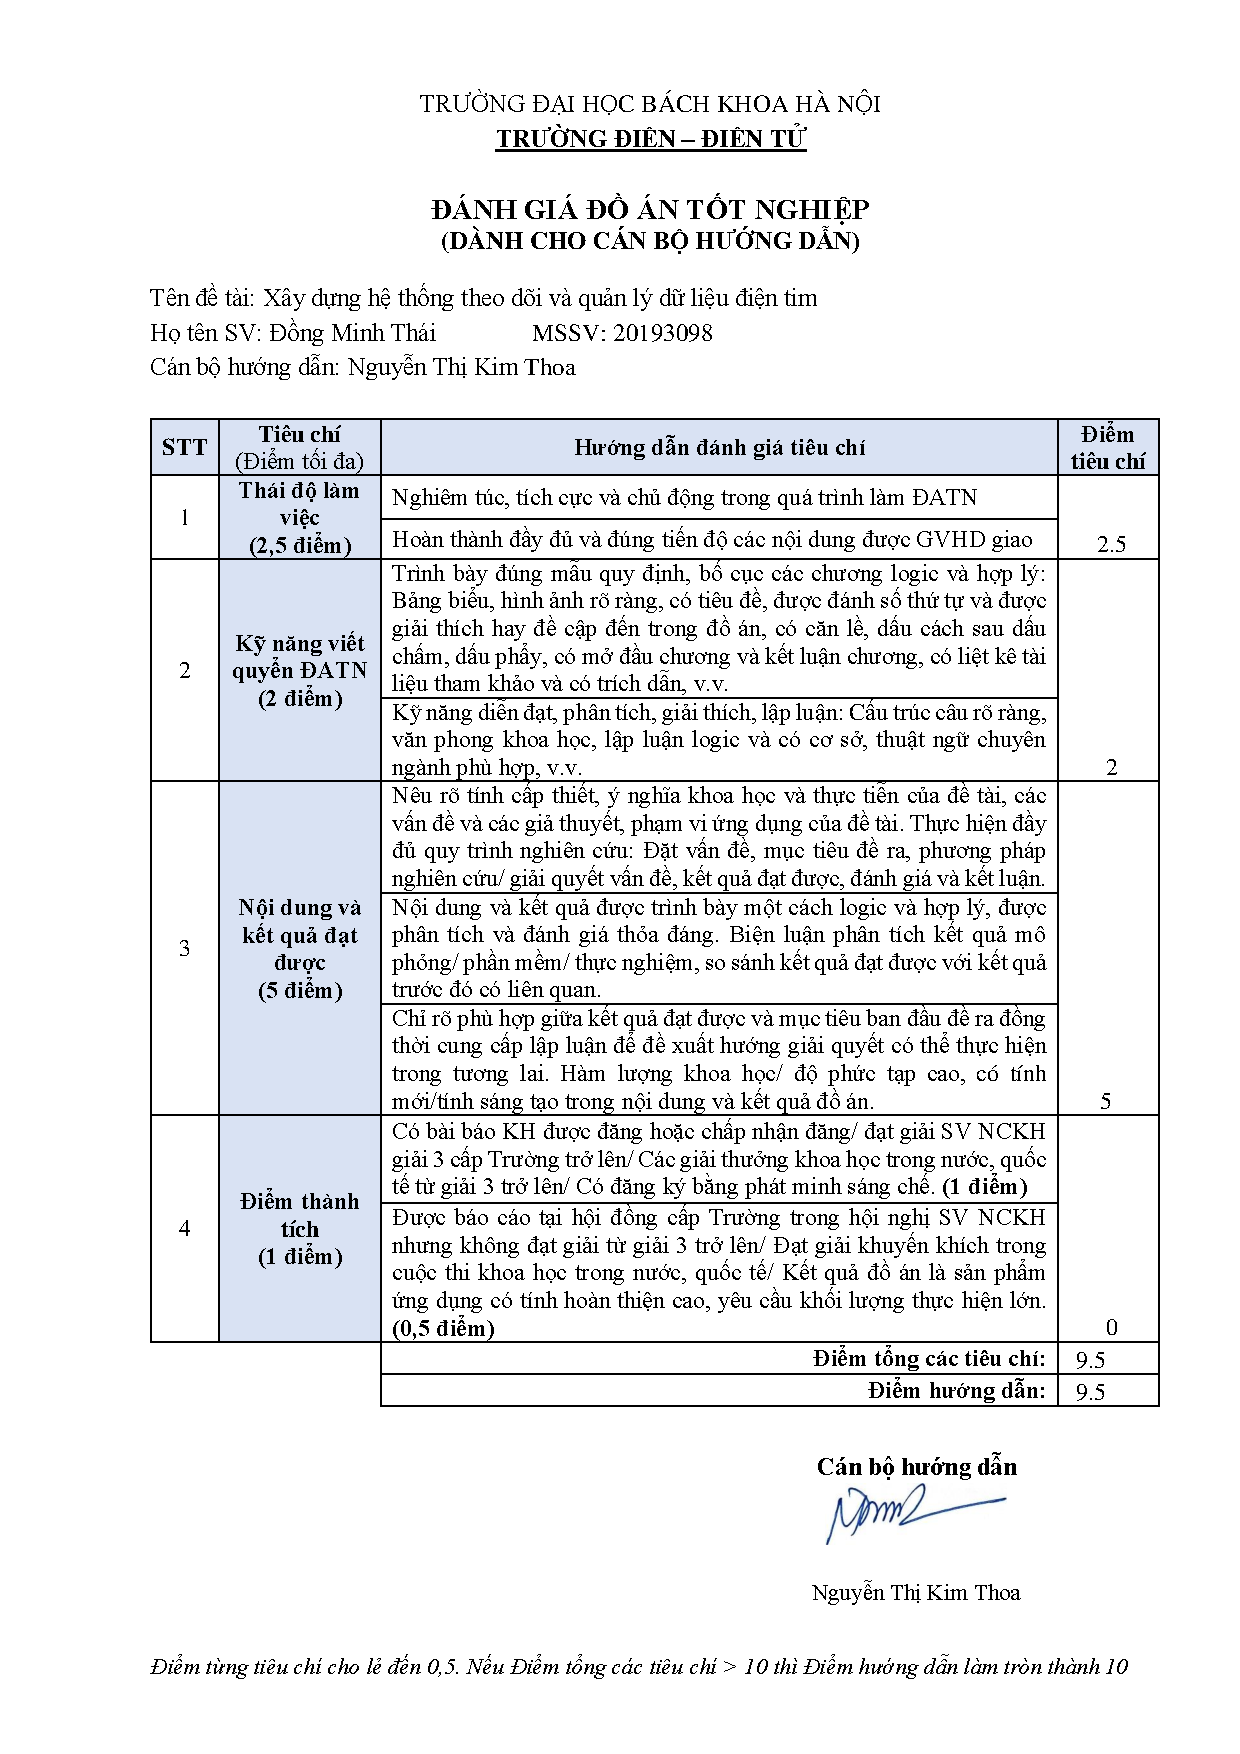
\includepdf[pages={1},scale=1]{PDF/SEEE_Evaluation_Dong_Minh_Thai.pdf}
% 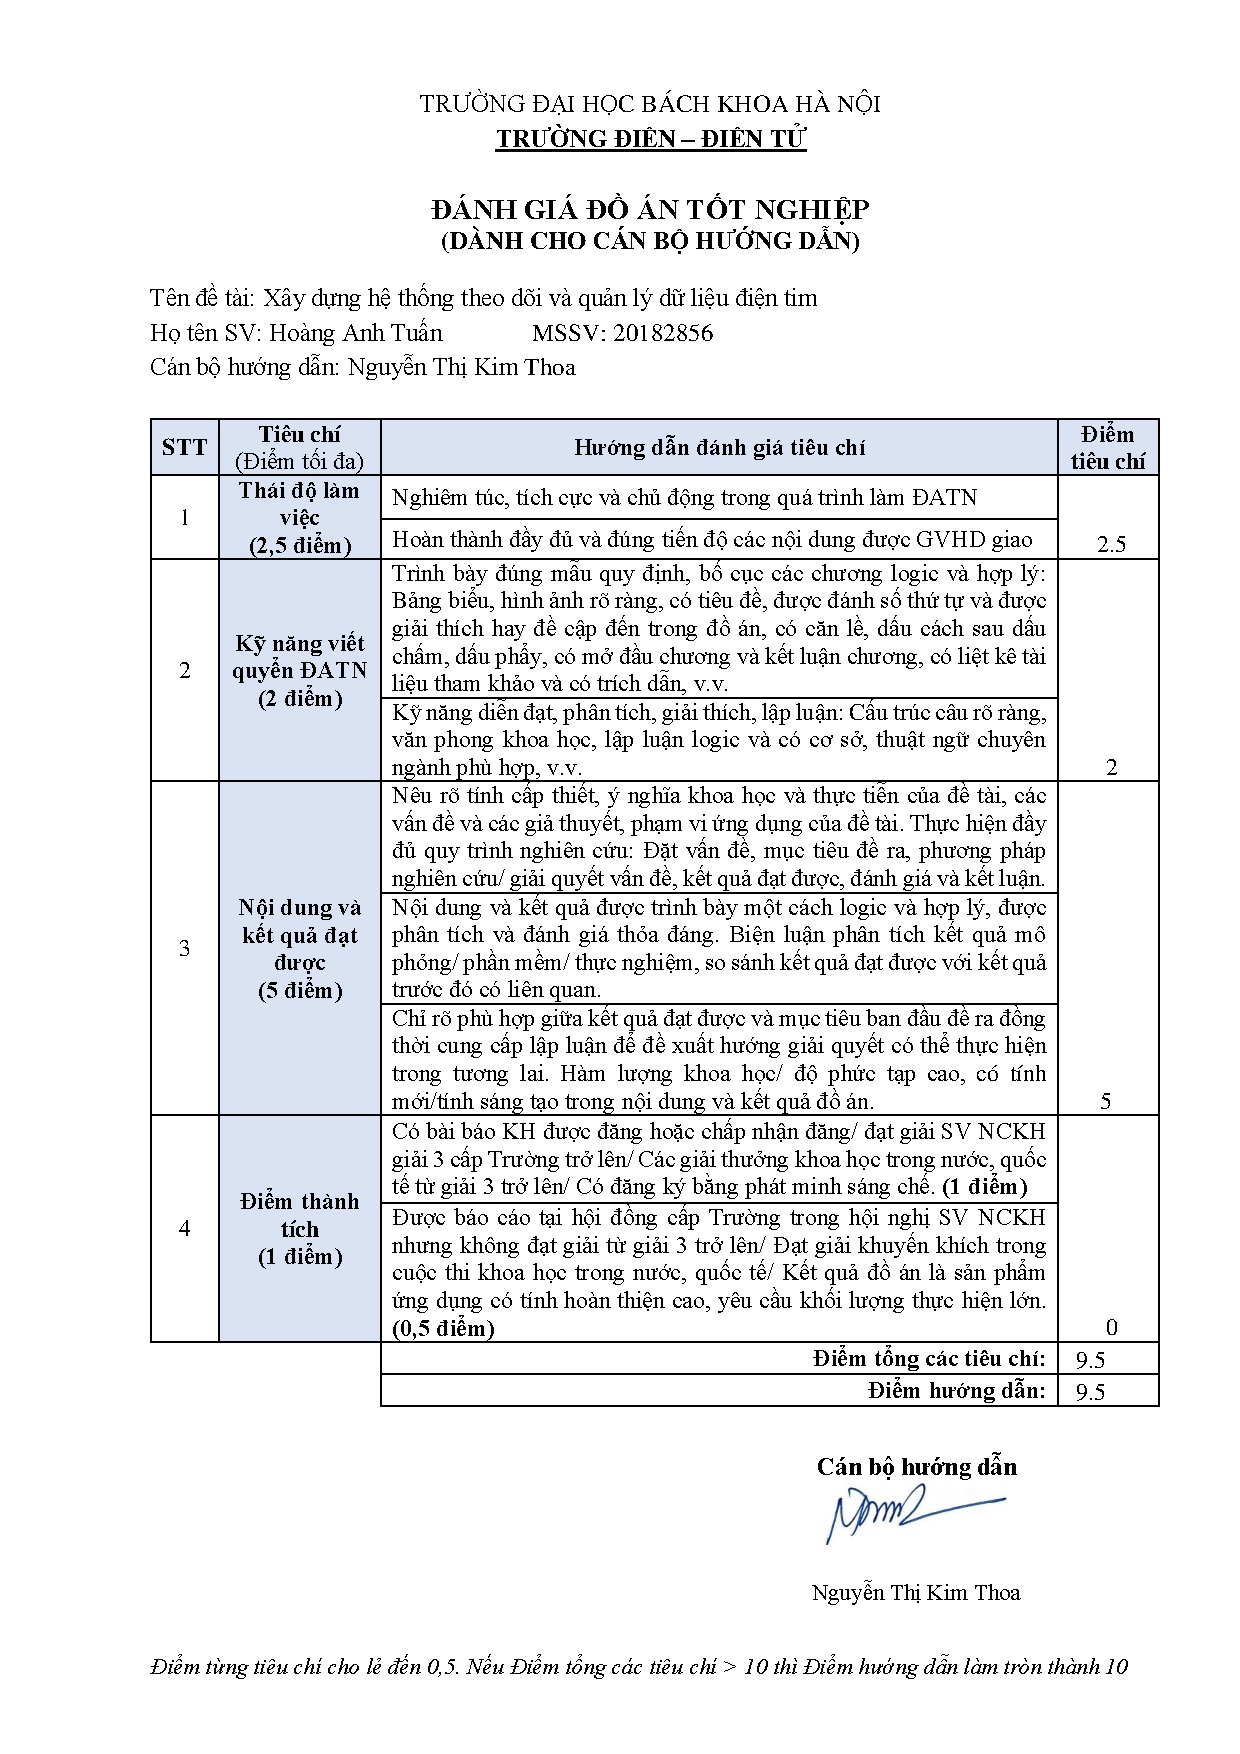
\includepdf[pages={1},scale=1]{PDF/SEEE_Evaluation_Hoang_Anh_Tuan.pdf}
% \cleardoublepage

% 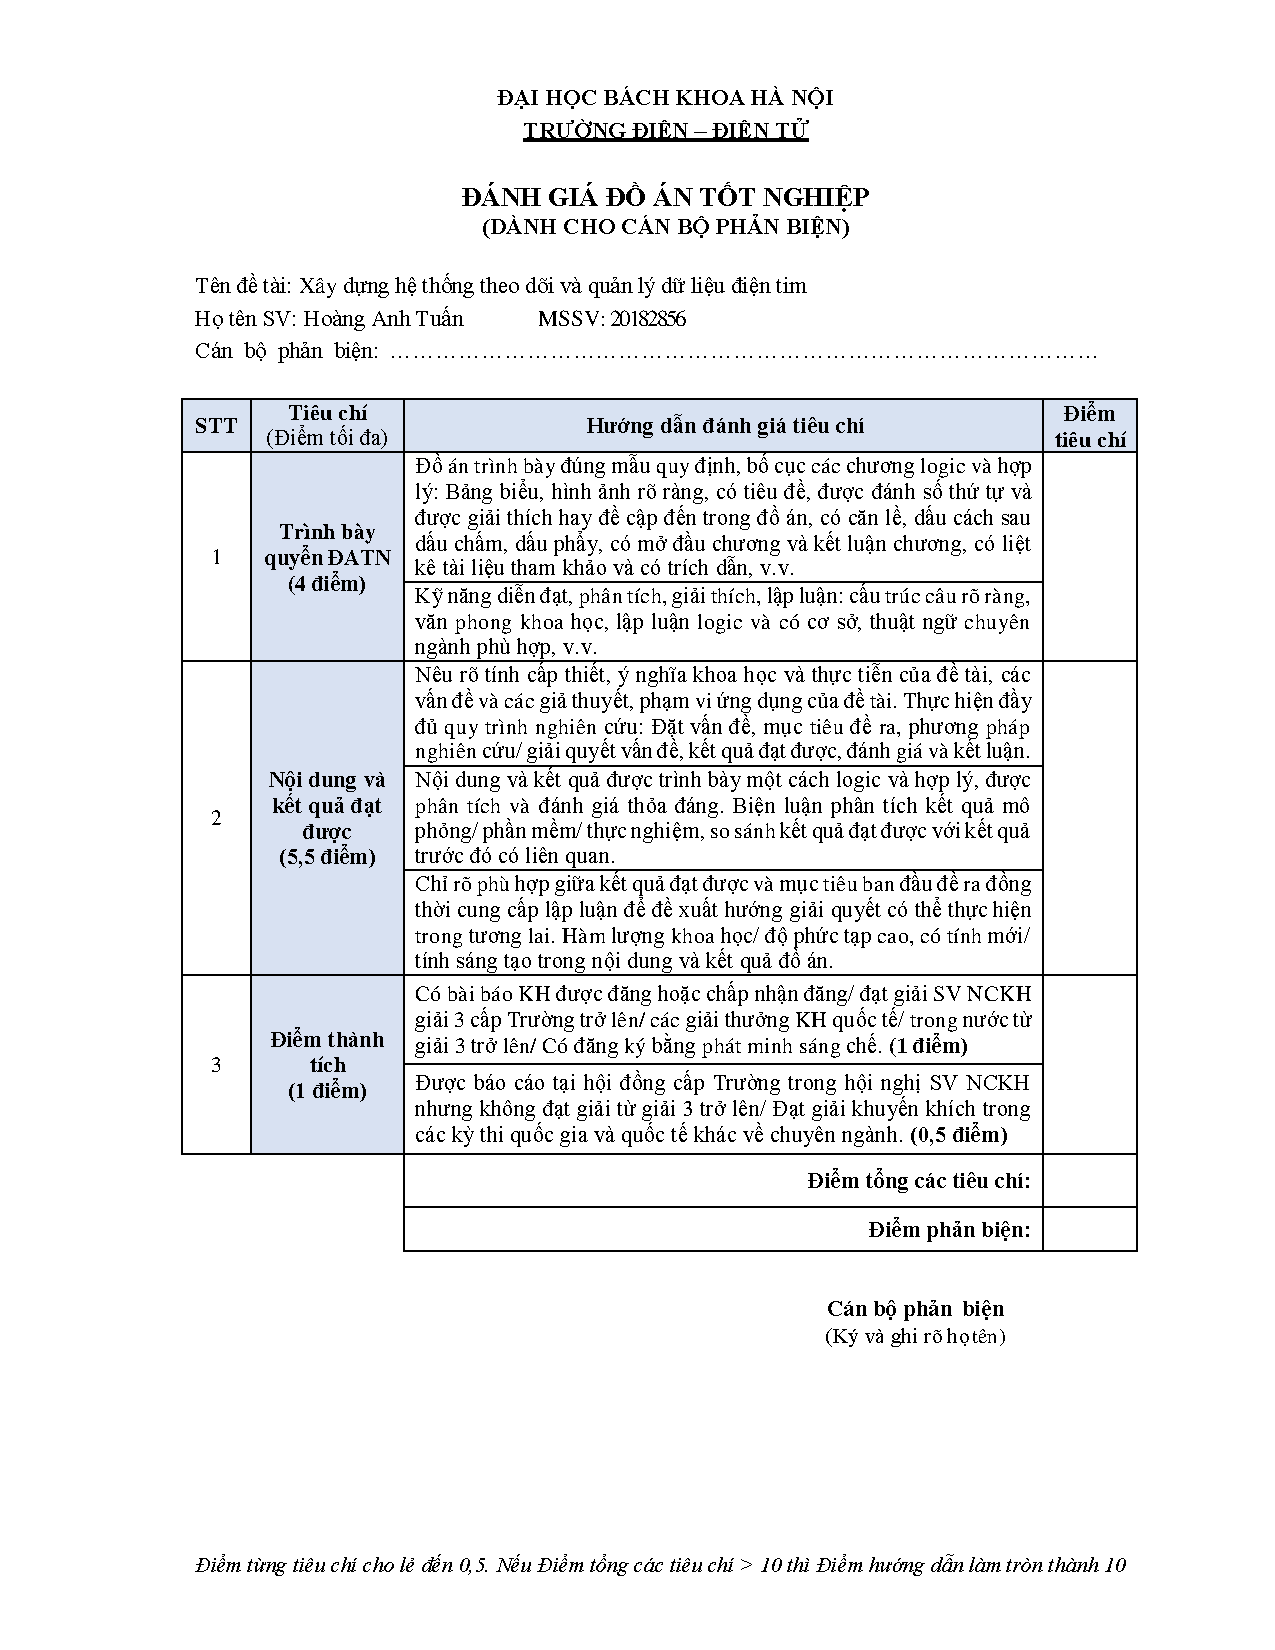
\includepdf[pages={1},scale=1]{PDF/SEEE_Danhgia2-anh_Tuan.pdf}
% 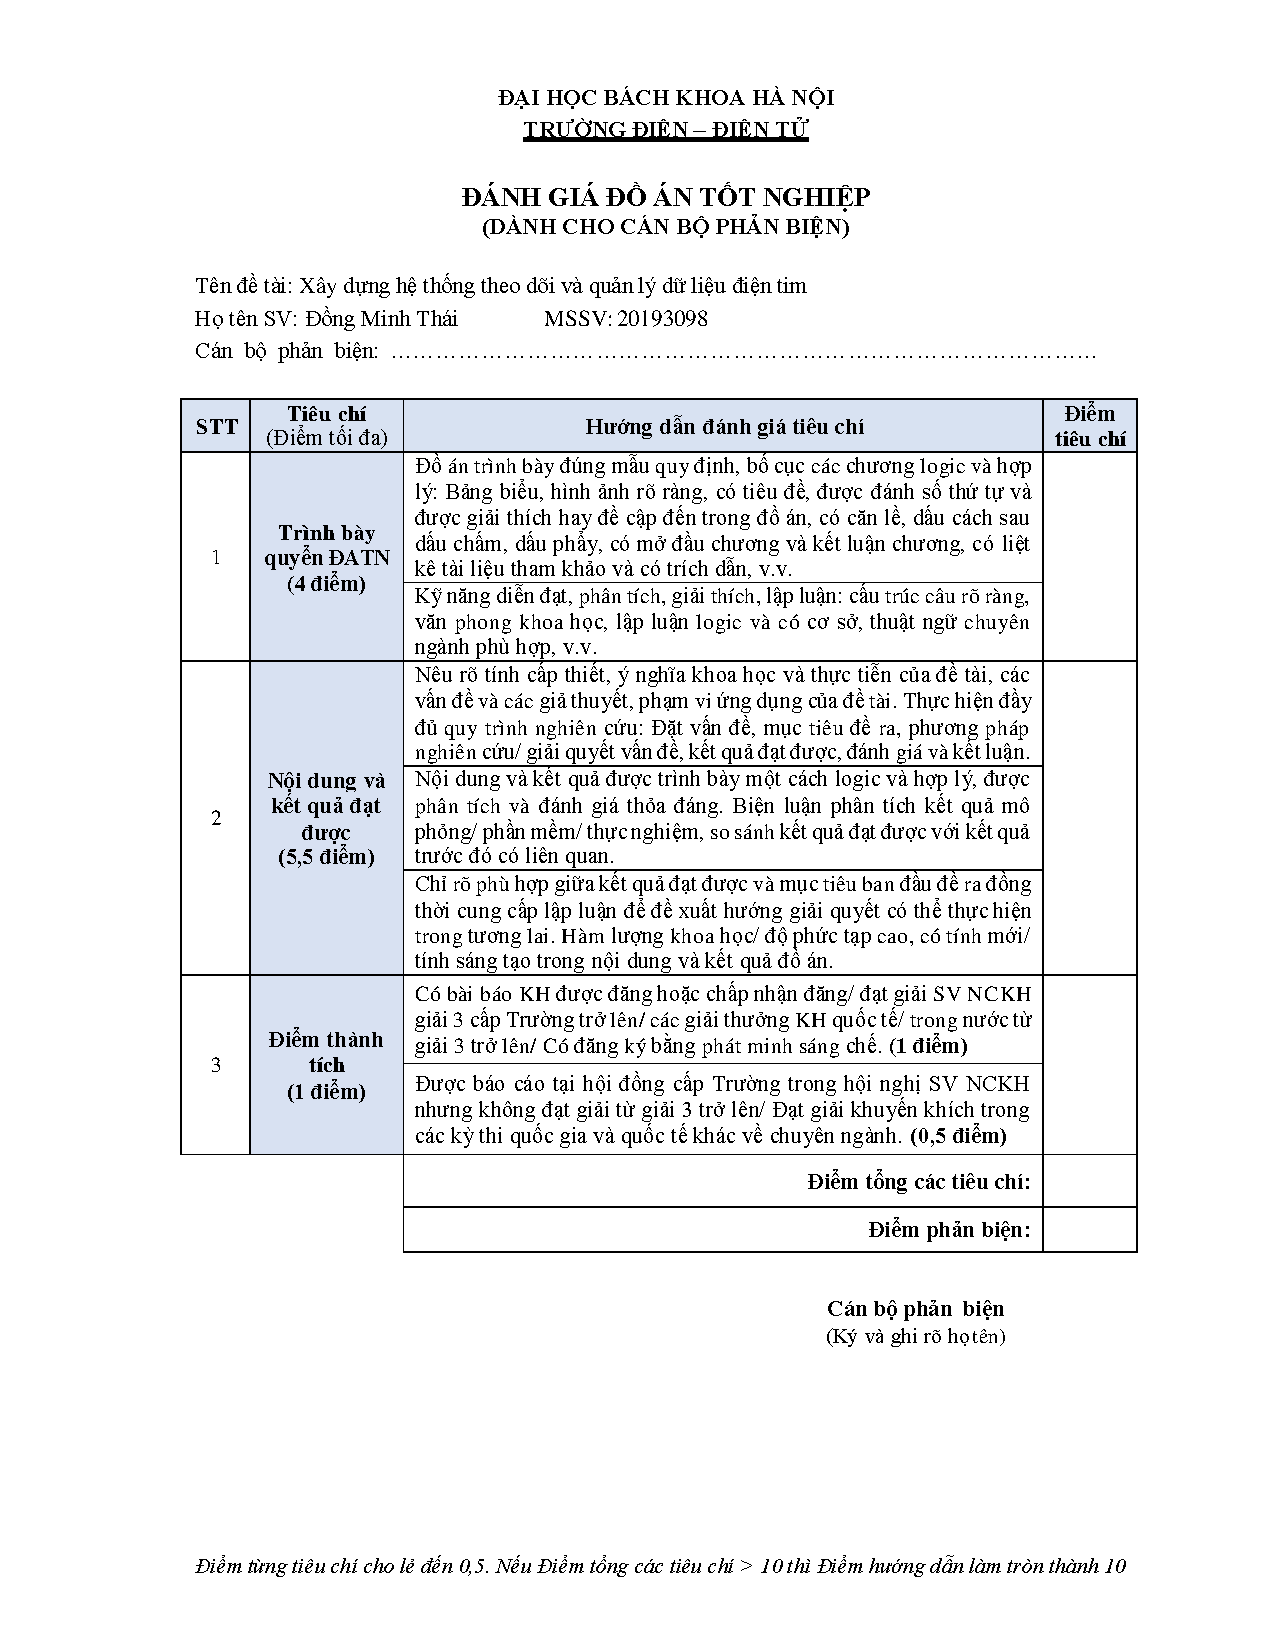
\includepdf[pages={1},scale=1]{PDF/SEEE_Danhgia2_Thai.pdf}
% \cleardoublepage

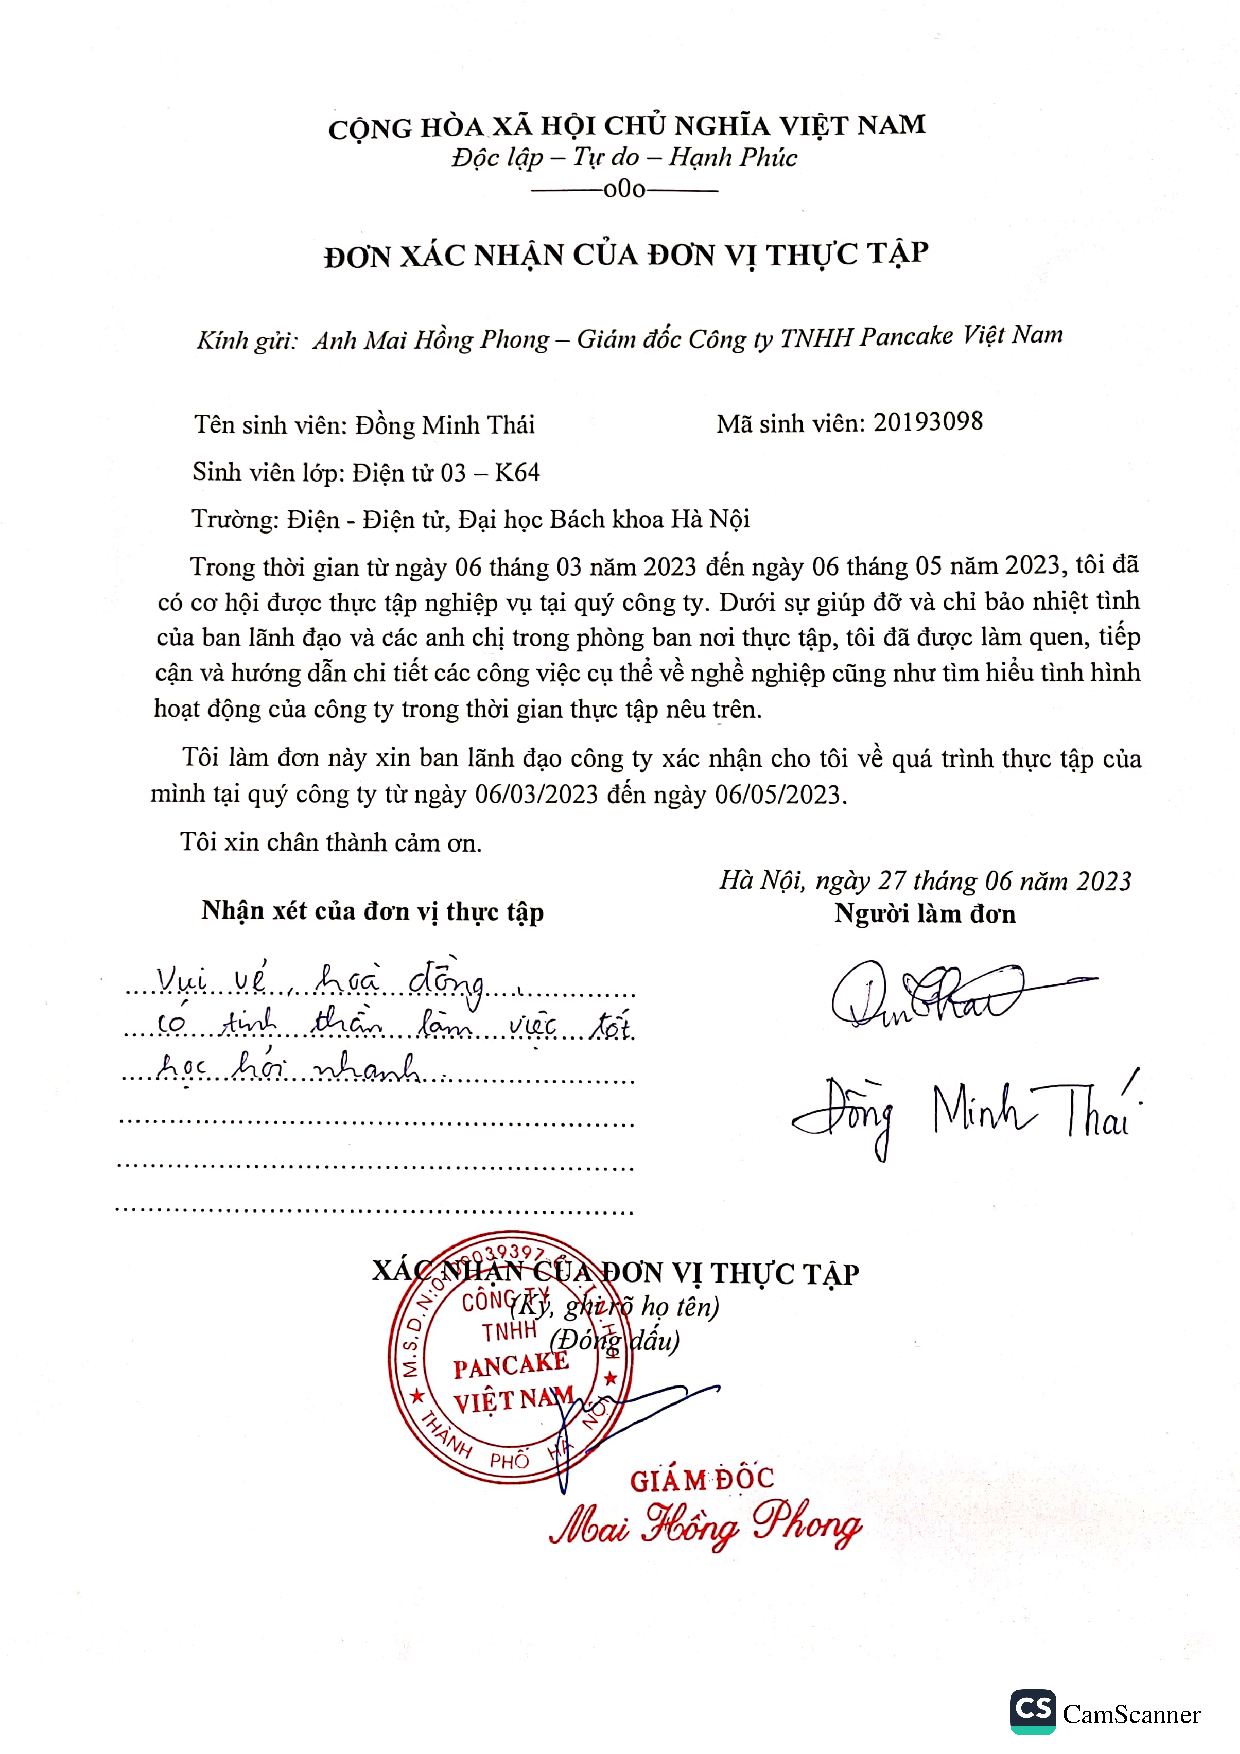
\includepdf[pages={1},scale=1]{PDF/don_xac_nhan_thuc_tap.pdf}
\cleardoublepage

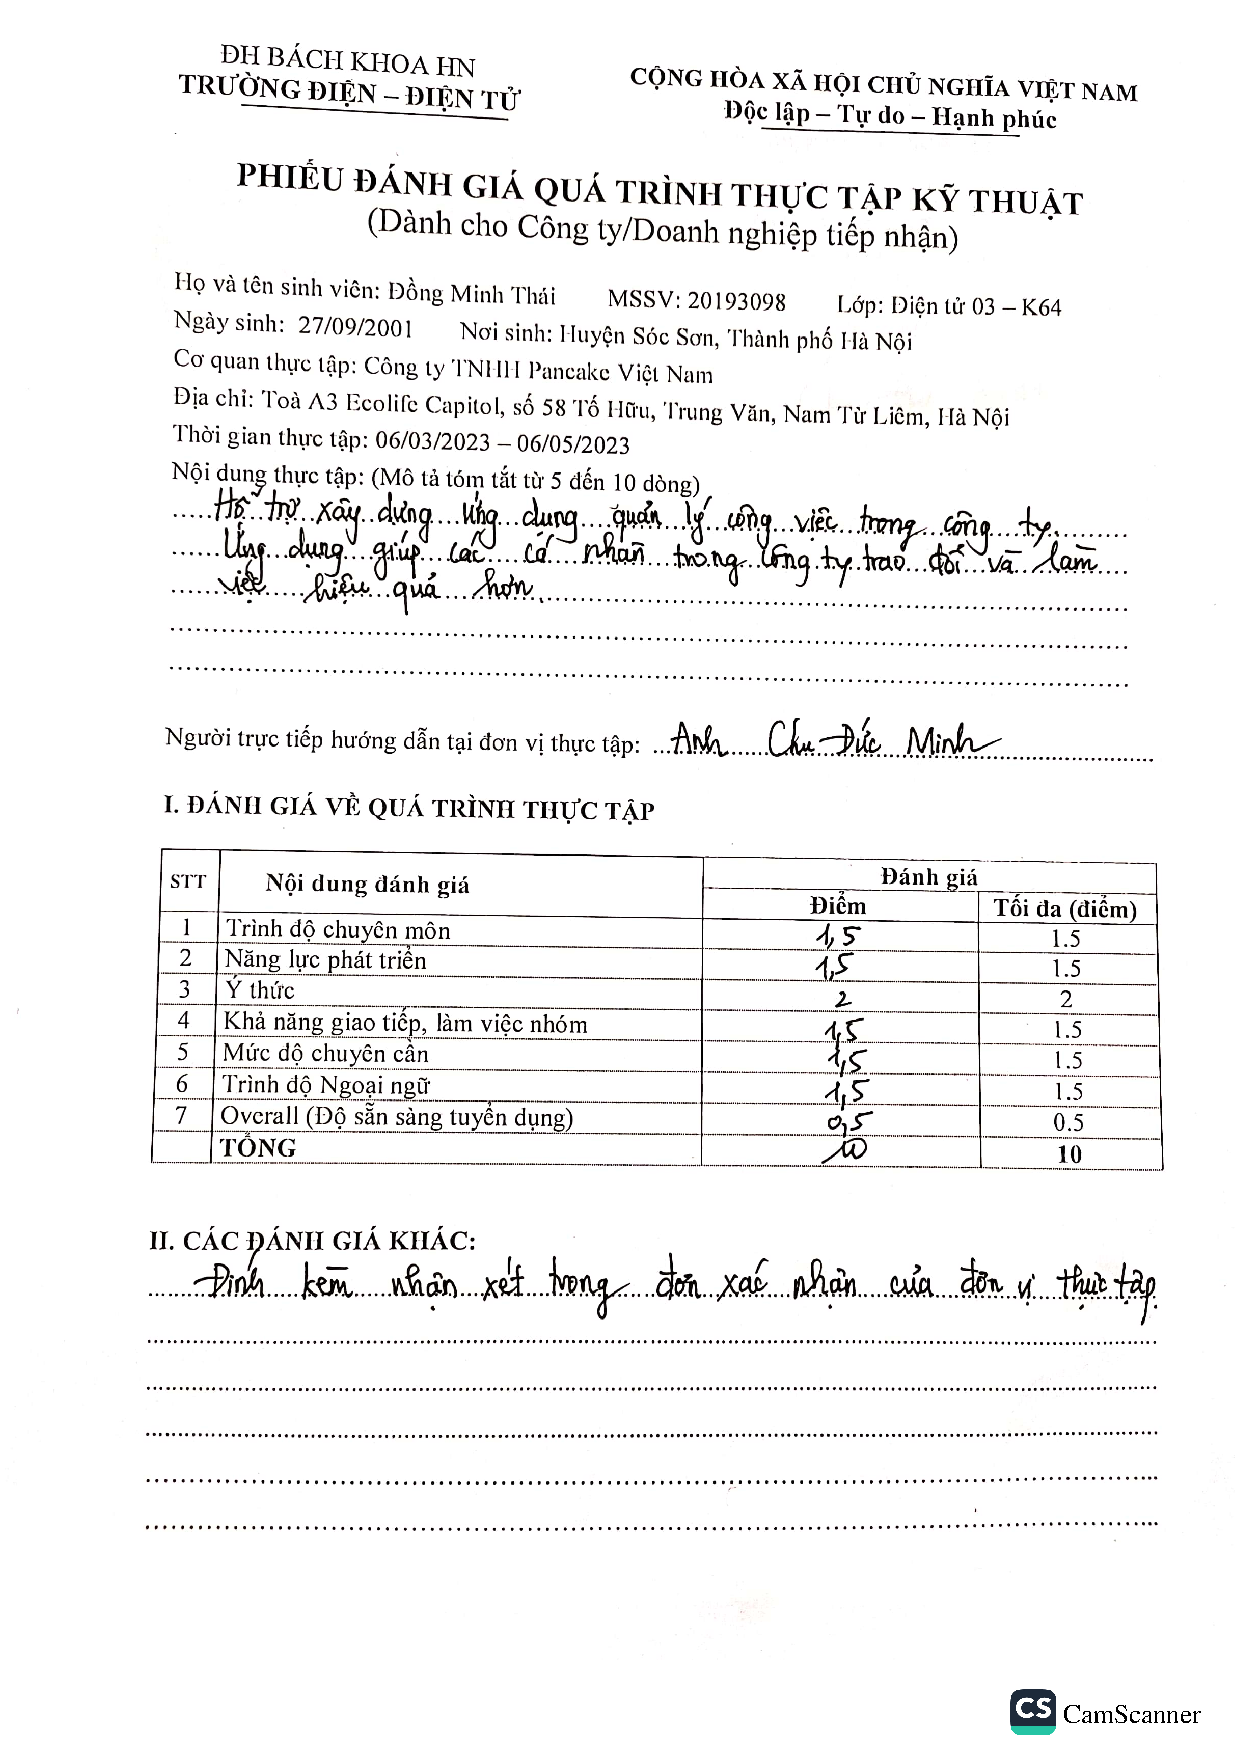
\includepdf[pages={1,2},scale=1]{PDF/danh_gia_thuc_tap.pdf}
% 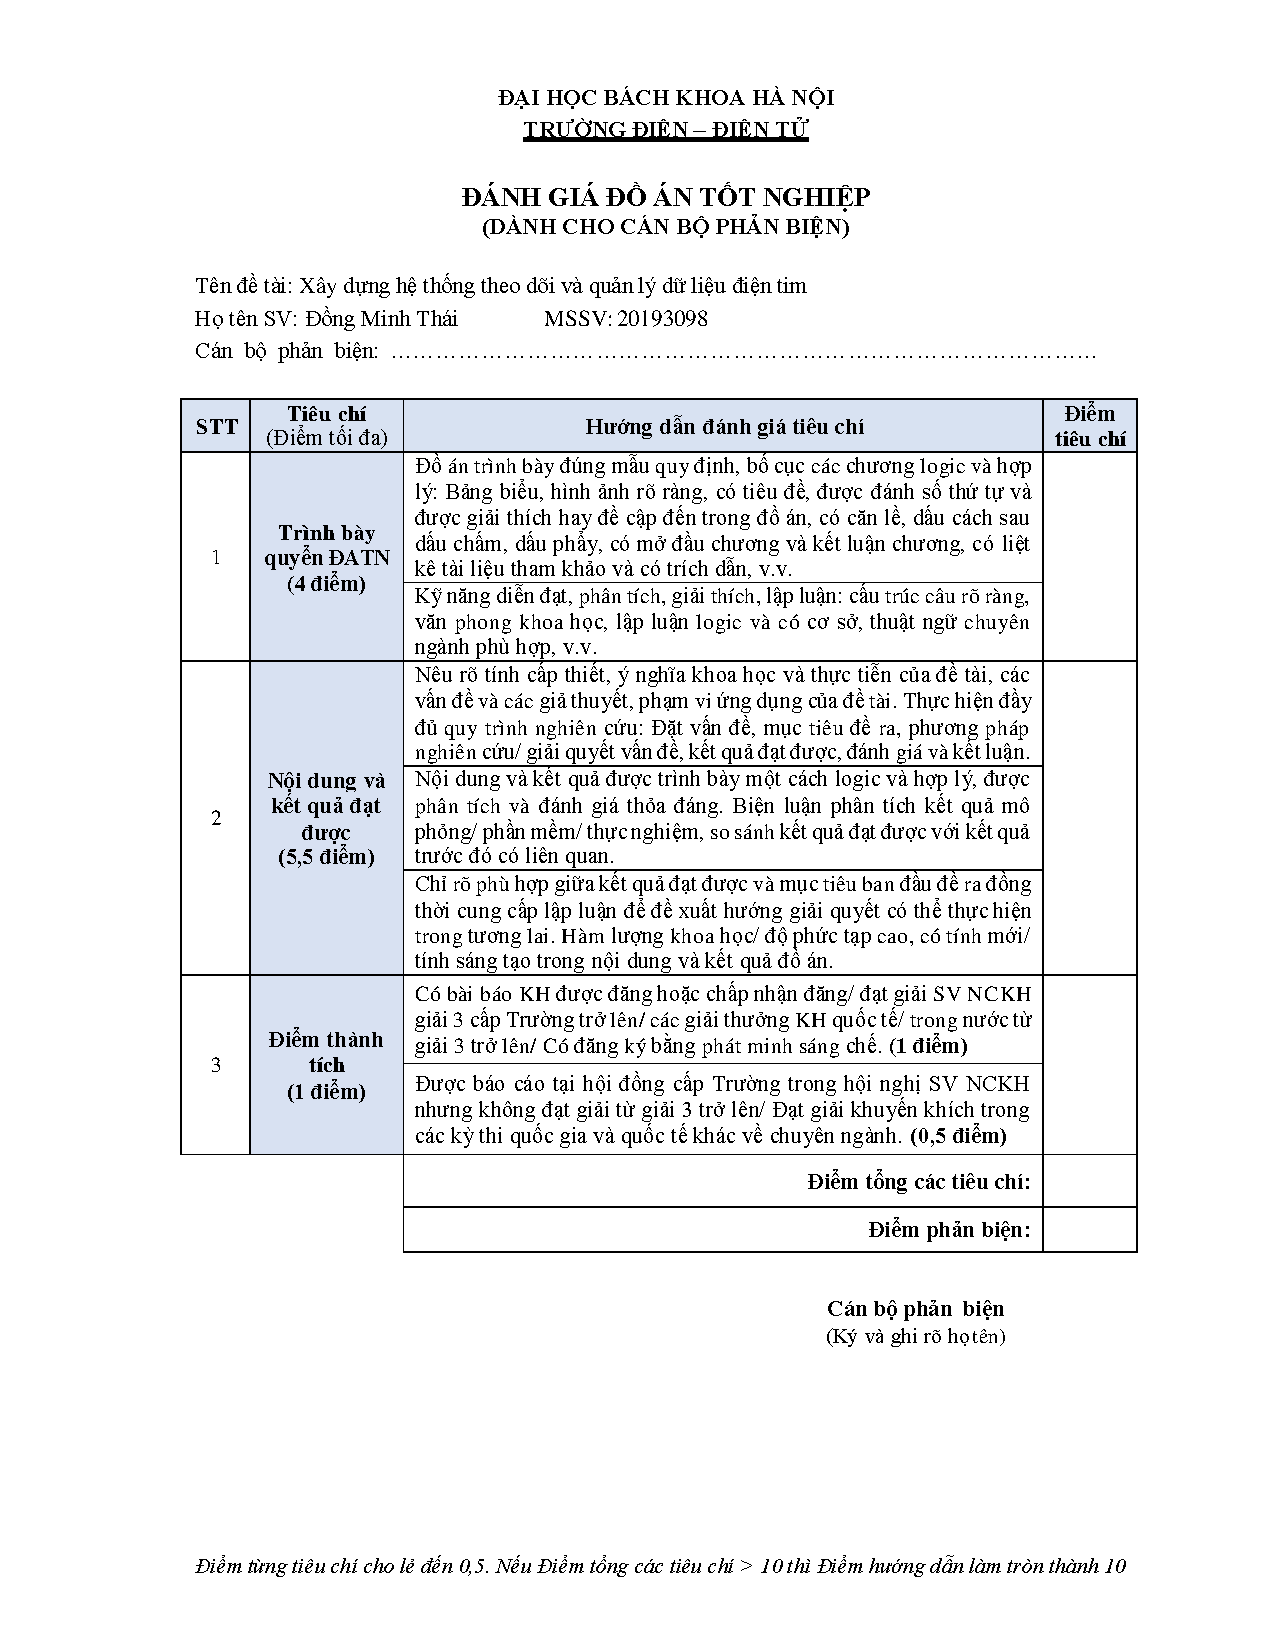
\includepdf[pages={1},scale=1]{PDF/SEEE_Danhgia2_Thai.pdf}
\cleardoublepage

\section*{LỜI NÓI ĐẦU} % dấu * để không đánh sô thứ tự vào lời nói đầu
\thispagestyle{empty}
Trong thời đại công nghệ phát triển vượt bậc, Internet vạn vật (IoT) ngày càng khẳng định vai trò quan trọng, đặc biệt trong lĩnh vực y tế. Việc áp dụng IoT vào quản lý thiết bị y tế không chỉ giúp tối ưu hóa quy trình chăm sóc sức khỏe mà còn mở ra những cơ hội đổi mới, nâng cao chất lượng dịch vụ y tế.
Tại Việt Nam, ứng dụng các công nghệ tiên tiến vào lĩnh vực y tế đóng vai trò quan trọng trong việc cải thiện sức khỏe cộng đồng, từ đó góp phần xây dựng nguồn nhân lực khỏe mạnh, đáp ứng yêu cầu phát triển đất nước.

Đồ án này của chúng em xây dựng một hệ thống trang web quản lý các thiết bị y tế và dữ liệu sức khỏe tim mạch, với mục tiêu tăng cường kết nối và hỗ trợ tương tác giữa bệnh nhân và bác sĩ.
Hệ thống cho phép bệnh nhân dễ dàng theo dõi tình trạng sức khỏe tại nhà, đồng thời nhận được sự hỗ trợ chuyên môn nhanh chóng từ đội ngũ y tế. Với giao diện thân thiện và dễ sử dụng, hệ thống tích hợp các chức năng hữu ích như đặt lịch hẹn, theo dõi dữ liệu sức khỏe tim mạch, và trao đổi thông tin trực tiếp giữa bệnh nhân và bác sĩ thông qua tính năng nhắn tin.

Trong quá trình thực hiện, chúng em đã nhận được sự hỗ trợ và hướng dẫn tận tình từ các thầy cô cùng sự giúp đỡ của các anh/chị/bạn tại các phòng thí nghiệm thuộc khoa Điện - Điện tử. Đặc biệt, chúng em xin bày tỏ lòng biết ơn sâu sắc đến TS. Hàn Huy Dũng, người đã luôn đồng hành và đưa ra những góp ý quý báu trong việc hoàn thiện đồ án.
Đồng thời, sự phối hợp cùng nhóm firmware của SPARC Lab đã giúp chúng em tích lũy được nhiều kiến thức và kinh nghiệm thực tế.

Dẫu đã nỗ lực hoàn thiện, đồ án của chúng em chắc chắn vẫn còn một số hạn chế. Chúng em rất mong nhận được những ý kiến đóng góp từ thầy cô và bạn đọc để tiếp tục phát triển và nâng cao chất lượng đề tài trong tương lai.

Chúng em xin chân thành cảm ơn!



\cleardoublepage

% \section*{LỜI CAM ĐOAN} % dấu * để không đánh sô thứ tự vào lời nói đầu
\thispagestyle{empty}

Chúng em gồm Cồ Huy Dũng, mã số sinh viên 20213834, thuộc lớp Điện tử 02, khóa K66, và Nguyễn Đức Dương, mã số sinh viên 20210259, thuộc lớp Điện tử 08, khóa K66.

Chúng em xin khẳng định rằng toàn bộ nội dung được trình bày trong đồ án "Hệ thống quản lý dữ liệu sức khỏe tim mạch và tương tác giữa bệnh nhân - bác sĩ" là kết quả của quá trình tìm hiểu, nghiên cứu và thực hiện nghiêm túc của chính chúng em.
Các thông tin, dữ liệu trong đồ án được đảm bảo tính trung thực và chính xác. Mọi tài liệu tham khảo đều được trích dẫn đầy đủ, tuân thủ các quy định về sở hữu trí tuệ. 

Chúng em xin cam kết chịu trách nhiệm hoàn toàn về nội dung đã trình bày trong đồ án này.


\vspace{6pt}

\hspace{8cm}Hà Nội, ngày 10 tháng 02 năm 2024

\hspace{9.8cm}\textbf{Người cam đoan}

\vspace{2cm}
\hspace{7.3cm}\textbf{NGUYỄN ĐỨC DƯƠNG,  CỒ HUY DŨNG}

\cleardoublepage
% \section*{PHÂN CÔNG CÔNG VIỆC} % dấu * để không đánh sô thứ tự vào lời nói đầu
\thispagestyle{empty}


\begin{table}[H]
  \centering
  
  \begin{tabularx}{0.9\textwidth}{
  | >{\raggedright\arraybackslash}m{1cm}
  | >{\raggedright\arraybackslash}X
  | >{\raggedright\arraybackslash}m{4cm}|
  }
  \hline
  \bfseries STT    &\bfseries Nội dung    &\bfseries Thành viên\\ \hline
  1   &   Tìm hiểu đề tài, đề xuất hệ thống  & Tuấn, Huy  \\ \hline
  2   &   Phân tích hệ thống  &  Tuấn, Huy \\ \hline
  3   &   Thiết kế cơ sở dữ liệu  & Tuấn, Huy  \\ \hline
  4   &   Thiết kế API & Tuấn \\ \hline
  5   &   Xây dựng phía back-end  & Tuấn, Huy \\ \hline
  6   &   Thiết kế website quản trị  & Huy \\ \hline
  7   &   Kiểm thử  &  Tuấ, Huy\\ \hline
  8   &   Viết quyển đồ án  & Tuấn, Huy  \\ \hline


  \end{tabularx}
  \label{table_api_pat_doc}
\end{table}




\cleardoublepage


% %mục lục
% \phantomsection\addtocontents{toc}{\protect\thispagestyle{empty}}
% \tableofcontents % tạo mục lục tự động
% \thispagestyle{empty}
% \thispagestyle{empty}
% \cleardoublepage


\clearpage
\pagestyle{empty} % Loại bỏ số trang trên các trang trong mục lục
\phantomsection
\addtocontents{toc}{\protect\thispagestyle{empty}}
% {%
\setstretch{1.2}
\tableofcontents % tạo mục lục tự động

\clearpage
\pagestyle{plain} % Khôi phục lại kiểu số trang cho các trang sau mục lục

\cleardoublepage

\pagenumbering{roman} %đánh số thứ tự la mã
\phantomsection\section*{DANH MỤC KÝ HIỆU VÀ CHỮ VIẾT TẮT}%dấu * để không đánh số
\addcontentsline{toc}{section}{\numberline{}DANH MỤC KÝ HIỆU VÀ CHỮ VIẾT TẮT} % LƯU VÀO TRONG MỤC LỤC

\begin{table}[H]
  \centering
  \begin{tabularx}{0.85\textwidth}{
  | >{\centering\arraybackslash}m{3cm}
  | >{\centering\arraybackslash}X|
  }
  \hline
  \bfseries Từ viết tắt     &\bfseries Thay cho\hspace{1cm}\\ \hline
  API     & Application Programming Interface \\ \hline
  JWT  & JSON Web Token \\ \hline
  ECG   & Electrocardiogram \\ \hline
  HTML   & Hypertext Markup Language \\ \hline
  ID    & Identification \\ \hline
  3NF   & Third Normal Form \\ \hline
  ERD     & Entity-Relationship Diagram \\ \hline
  AWS  & Amazon Web Services \\ \hline
  RDS   & Relational Database Service \\ \hline
  EC2   & Elastic Compute Cloud \\ \hline
  FPS   & Frames Per Second \\ \hline
  IOT   & Internet Of Things \\ \hline
  UML   & Unified Modeling Language \\ \hline
  PDA   & Patient Doctor Assignment \\ \hline
  CRC   & Class - Responsibility - Collaboration \\ \hline
  AI   & Artificial Intelligence \\ \hline
  GPT   & Generative Pre-trained Transformer \\ \hline




  
  \end{tabularx}
\end{table}
\cleardoublepage

{
\let\oldnumberline\numberline
\renewcommand{\numberline}{\figurename~\oldnumberline}%
\listoffigures
} %tạo danh mục hình vẽ tự động
\phantomsection\addcontentsline{toc}{section}{\numberline{}DANH MỤC KÝ HÌNH VẼ}
\cleardoublepage

{
\let\oldnumberline\numberline
\renewcommand{\numberline}{\tablename~\oldnumberline}%
\listoftables
} %tạo danh mục hình vẽ tự động %tạo danh mục bảng biểu
\phantomsection\addcontentsline{toc}{section}{\numberline{}DANH MỤC BẢNG BIỂU}
\cleardoublepage
% }%

% \section*{TÓM TẮT ĐỒ ÁN}
\phantomsection\addcontentsline{toc}{section}{\numberline{}TÓM TẮT ĐỒ ÁN}
Đồ án "Phát triển ứng dụng di động tích hợp trong hệ thống quản lý dữ liệu tim mạch, hỗ trợ kết nối giữa bệnh nhân - bác sĩ" là một hệ thống tích hợp bao gồm Web/App/Server, sử dụng công nghệ Bluetooth Low Energy để hỗ trợ việc theo dõi và quản lý dữ liệu điện tim trên ứng dụng di động một cách hiệu quả và tiện lợi. Dữ liệu sau mỗi phiên đo được lưu trữ trên server, cho phép người dùng xem lại bất kỳ lúc nào và phục vụ cho các mục đích nghiên cứu trong tương lai. Bên cạnh đó, hệ thống còn cung cấp các tính năng hỗ trợ kết nối trực tiếp giữa bệnh nhân và bác sĩ, như đặt lịch hẹn, nhắn tin trao đổi thông tin và theo dõi dữ liệu sức khỏe, mang lại sự tiện ích và chuyên nghiệp trong quản lý sức khỏe.

Trong đồ án, nhóm tập trung hoàn thiện hệ thống theo quy trình phát triển phần mềm, từ việc xác định các yêu cầu hệ thống đến phân tích, thiết kế và triển khai. Quy trình này áp dụng phương pháp phân tích và thiết kế hướng đối tượng, sử dụng ngôn ngữ UML để biểu diễn các luồng thực hiện hành động. Về mặt kỹ thuật, ứng dụng di động được phát triển trên hệ điều hành Android và iOS sử dụng Flutter Framework, trong khi ứng dụng Web được xây dựng với ReactJS và AdminJS. Server của hệ thống sử dụng NodeJS, framework NestJS, và được triển khai trên Amazon EC2. Hệ thống sử dụng cơ sở dữ liệu MySQL kết hợp với NoSQL (MongoDB) để đảm bảo hiệu năng và khả năng lưu trữ linh hoạt.

Quyển đồ án được trình bày theo quy trình phát triển phần mềm, với nội dung được triển khai chi tiết trong từng chương, bao gồm: phân tích hệ thống, thiết kế hệ thống, triển khai và kiểm thử, và cuối cùng là phần kết luận. Tất cả các nội dung được minh họa bằng sơ đồ và các diễn giải cụ thể, đảm bảo tính rõ ràng và khoa học.
% \cleardoublepage

\newpage
\section*{ABSTRACT}
% \phantomsection\addcontentsline{toc}{section}{\numberline{}ABSTRACT}
The project "Development of a Mobile Application Integrated into a Cardiovascular Data Management System, Supporting Patient-Doctor Connectivity" is an integrated system comprising Web/App/Server, leveraging Bluetooth Low Energy (BLE) technology to facilitate effective and convenient monitoring of electrocardiogram (ECG) data through a mobile application. The data collected after each measurement session is stored on the server, enabling users to review it at any time and supporting future research purposes. Furthermore, the system provides features that enhance direct connectivity between patients and doctors, including appointment scheduling, messaging for information exchange, and health data monitoring, delivering convenience and professionalism in healthcare management.

This project focuses on completing the system following a software development lifecycle (SDLC), starting from identifying system requirements to analyzing, designing, and implementing the solution. The development process applies object-oriented analysis and design (OOAD) methodologies, utilizing Unified Modeling Language (UML) to represent action flows. From a technical perspective, the mobile application is developed for both Android and iOS platforms using the Flutter framework. The web application is built with ReactJS and AdminJS, while the server utilizes NodeJS and the NestJS framework, deployed on Amazon EC2. The system employs MySQL in combination with NoSQL (MongoDB) databases to ensure both performance and flexible data storage capabilities.

The project documentation is structured according to the software development lifecycle, with detailed content presented in individual chapters, including system analysis, system design, implementation, testing, and finally, conclusions. All content is illustrated with diagrams and comprehensive explanations, ensuring clarity and scientific rigor.

\cleardoublepage




% 
\section*{PHẦN MỞ ĐẦU}
\phantomsection\addcontentsline{toc}{section}{\numberline{} PHẦN MỞ ĐẦU}
\subsection*{Đặt vấn đề}

% \addcontentsline{toc}{section}{\numberline{} Đặt vấn đề}
% Cuộc cách mạng công nghiệp lần thứ tư (hay còn được gọi là cuộc cách mạng công nghiệp 4.0) đã và đang phát triển với tốc
% độ rất nhanh, ảnh hưởng đến mọi mặt đời sống xã hội. Nội dung cốt lõi của cuộc cách mạng chính là sự kết hợp giữa 
% khoa học công nghệ, trí tuệ nhân tạo và sự sáng tạo của con người. Đối với Việt Nam đang trong quá trình công nghiệp hoá, 
% hiện đại hoá, việc áp dụng được những công nghệ mới trong một số lĩnh vực thiết yếu của xã hội, đặc biệt trong ngành y tế, 
% chính là nền tảng quan trọng để chăm sóc sức khoẻ con người, từ đó tạo nên những con người với sức khoẻ tốt nhất, sẵn sàng 
% đóng góp cho sự phát triển của đất nước. 
Lĩnh vực y tế đang có những bước chuyển mình lớn trong cuộc cách mạng công nghiệp lần thứ tư 
(hay còn được gọi là cuộc cách mạng công nghiệp 4.0). Đại dịch COVID-19 đã chứng minh được tầm quan trọng của việc áp dụng
khoa học kỹ thuật vào những sản phẩm y tế giúp đẩy lùi dịch bệnh,
có thể kể đến như máy rửa tay tự động do TS.Hàn Huy Dũng (đang công tác tại Trường Điện - Điện tử, thuộc Đại học Bách khoa Hà Nội) 
cùng các cộng sự sáng chế \cite{ref_thay_dzung}, và một số ứng dụng di động
nổi bật được hầu hết người dân Việt Nam sử dụng trong đại dịch COVID-19 như Bluezone - ứng dụng cảnh báo tiếp xúc gần với
những người nhiễm COVID qua Bluetooth low energy, ứng dụng NCOVI, theo dõi các ca nhiễm và thực hiện khai báo y tế, ứng
dụng PC-Covid để cập nhật các thông tin tiêm vắc xin, thông tin xét nghiệm. Đây là một tín hiệu cho thấy nước ta đang áp
dụng công nghệ 4.0 vào trong ngành y tế một cách chủ động. Hiện nay, việc chăm sóc sức khoẻ đang được chú trọng, đối với 
những những người muốn tự theo dõi sức khoẻ bản thân
thì các thiết bị nhỏ gọn có chức năng hỗ trợ đo và một ứng dụng di động hỗ trợ việc theo dõi sức khoẻ là một trong những
điều quan trọng và cần thiết. Kể cả đối với những người gặp vấn đề về sức khoẻ, việc đến bệnh viện đông đúc để theo dõi
và khám là khá khó khăn. Câu hỏi đặt ra là có phương án khả thi nào có thể áp dụng cho việc chăm sóc sức khoẻ một cách cụ thể, 
người dùng vẫn có thể theo dõi sức khoẻ tại nhà, đồng thời có sự cố vấn và hỗ trợ của những người có chuyên môn không?

\subsection*{Đề xuất hệ thống}
% \phantomsection\addcontentsline{toc}{section}{\numberline{} Đề xuất hệ thống}

Trong mục Đặt vấn đề, chúng em có trình bày về vấn đề chăm sóc sức khoẻ tại nhà, ở mục này, chúng em xin phép đề xuất một hệ thống
dựa trên những tiến bộ của khoa học kĩ thuật, với sự kết hợp giữa thiết bị IOT cùng hệ thống ứng dụng theo dõi, lưu trữ,
giúp tiết kiệm thời gian cũng như tăng khả năng tiếp cận cho nhiều người dùng. 

Với nền tảng được tiếp cận thiết bị đo điện tim bằng điện cực không tiếp xúc trong thời gian gần đây, 
cùng với đó là việc phát triển các thiết bị IOT đang rất được chú trọng hiện nay, chúng em mong muốn xây dựng được một hệ thống
có thể kết nối được các thiết bị đo điện tim, thu thập dữ liệu điện tim thời gian thực, đồng thời có thể lưu trữ và phục vụ cho mục đích
phân tích dữ liệu về sau này. Cụ thể, hệ thống sẽ bao gồm:

\begin{adjustwidth}{1.5em}{}
  \begin{itemize}
      \item Một ứng dụng di động dành riêng cho người dùng có thể kết nối với thiết bị đo điện tim để theo dõi trực tiếp tình trạng sức khoẻ, đồng
      thời có thể trao đổi với bác sĩ về tình trạng sau các lần đo, xem tin tức về các thông tin liên quan tới sức khoẻ
      \item Một ứng dụng di động cho bác sĩ để có thể xem được kết quả đo của các bệnh nhân được quản lý, trao đổi được với bệnh nhân
      \item Một ứng dụng web cho admin để quản lý hệ thống, đặc biệt là có phần phân công bác sĩ quản lý cho bệnh nhân, xem được thông tin thiết bị đang có cũng như theo dõi kết quả đo
      \item Một server để lưu cơ sở dữ liệu liên quan đến người dùng và dữ liệu đo của bệnh nhân, có thể phục vụ cho công tác nghiên cứu và
      phân tich dữ liệu sau này
  \end{itemize}
  \end{adjustwidth}


\subsection*{Mục tiêu của đề tài}
Sau khi đã trình bày đề xuất về một hệ thống theo dõi và quản lý dữ liệu điện tim, mục tiêu đặt ra khi thực hiện
đề tài này đó là:

\begin{adjustwidth}{1.5em}{}
  \begin{itemize}
      \item Nắm được cơ sở lý thuyết và cách thiết kế, ứng dụng các thiết bị trong hệ thống IOT
      \item Thực hiện hoàn chỉnh các ứng dụng được đề ra trong mục Đề xuất hệ thống, các ứng dụng hoạt động ổn định
      \item Có thể kết hợp tốt với các thiết bị phần cứng đang được hợp tác nghiên cứu
      \item Cung cấp tài liệu tham khảo một cách đầy đủ, trung thực

  \end{itemize}
  \end{adjustwidth}





\subsection*{Phương pháp nghiên cứu}
Trong đồ án lần này, chúng em đã thực hiện kết hợp các phương pháp nghiên cứu, đầu tiên là tham khảo thông tin các bài
báo, sản phẩm về thiết bị điện tim trong các phòng nghiên cứu tại trường, cùng với đó, tìm hiểu cách các hệ thống phần cứng và phần mềm hoạt động,
kết nối với nhau. Sau khi đã nắm được cơ sở lý thuyết, chúng em tiến hành các bài thực nghiệm, thử kết nối bluetooth, truyền dữ liệu với các điều kiện khác nhau,
kết hợp với nhóm firmware để phân tích số liệu nhằm chắc chắn dữ liệu được truyền đúng.

\subsection*{Kết quả đạt được}

Trong suốt quá trình thực hiện đồ án, hai chúng em Trần Minh Tuấn, Phạm Quang Huy đã được tìm hiểu và nghiên cứu sâu hơn về cả phần cứng,
hệ thống IOT, cách kết nối các hệ thống với nhau. Các kết quả đạt được cho đến thời điểm hoàn thiện quyển đồ án bao gồm:

\begin{adjustwidth}{1.5em}{}
  \begin{itemize}
      \item Hoàn thành quyển đồ án với nội dung chi tiết về quá trình xây dựng và phát triển hệ thống
      \item Hoàn thành các sản phẩm ứng dụng đã đề ra trong mục Đề xuất hệ thống, các sản phẩm đã có sự kết nối, dữ liệu điện tim được theo dõi
      thời gian thực được lưu trên server, dữ liệu có thể được phân tích và nghiên cứu sau này
      \item Được phát triển các kỹ năng làm việc nhóm, viết đồ án, kết hợp với nhóm phần cứng, nhóm firmware để các sản phẩm được hoàn thiện hơn
    \end{itemize}
  \end{adjustwidth}
\subsection*{Cấu trúc đồ án}

% \phantomsection\addcontentsline{toc}{section}{\numberline{} Cấu trúc đồ án}
\begin{adjustwidth}{1.5em}{}
\begin{itemize}
  \item Phần mở đầu: Trình bày về mục đích của đồ án, đề xuất hệ thống, phần tích tính khả thi và bố cục đồ án
  \item Chương 1: Trình bày chi tiết các khâu thu thập yêu cầu. Bao gồm kĩ thuật thu thập, xác định yêu cầu hệ thống, thiết kế sơ đồ use case
  \item Chương 2: Trình bày chi tiết các khâu trong phân tích hệ thống. Bao gồm mô tả thẻ CRC, thiết kế sơ đồ lớp, sơ đồ tuần tự
  \item Chương 3: Trình bày chi tiết khâu thiết kế cho hệ thống. Bao gồm thiết kế sơ đồ kiến trúc hệ thống, sơ đồ khối
  phần mềm, thiết kế cơ sở dữ liệu, thiết kế giao diện, sơ đồ lớp và thiết kế chức năng cho hệ thống
  \item Chương 4: Trình bày khâu triền khai và kiểm thử
  \item Chương 5: Kết luận và nêu ra hướng phát triển
\end{itemize}
\end{adjustwidth}

\cleardoublepage

% \pagenumbering{arabic}

\pagenumbering{arabic}

\section*{CHƯƠNG 1. THU THẬP YÊU CẦU}
\setcounter{section}{1}
\setcounter{subsection}{0} %LƯU Ý MỖI LẦN THÊM CHƯƠNG MỚI CẦN THÊM CÂU NÀY ĐỂ RESET THỨ TỰ CỦA SUBSECTON VỀ 1
\setcounter{table}{0} % LƯU Ý SAU MỖI LẦN GỌI BẢNG HAY HÌNH ẢNH PHẢI THÊM CÂU NÀY ĐỂ RESET THỨ TỰ
\setcounter{figure}{0} %% LƯU Ý SAU MỖI LẦN GỌI BẢNG HAY HÌNH ẢNH PHẢI THÊM CÂU NÀY ĐỂ RESET THỨ TỰ
\addcontentsline{toc}{section}{\numberline{}CHƯƠNG 1. THU THẬP YÊU CẦU}
Chương này sẽ tiến hành thu thập yêu cầu cho dự án đề tài "Hệ thống quản lý dữ liệu điện tim và tương tác giữa bênh nhân - bác sĩ"
dựa trên các mục tiêu đã nêu ra trong Mục Đề xuất hệ thống ở Phần mở đầu.

\subsection{Yêu cầu hệ thống}
\subsubsection{Yêu cầu về người dùng hệ thống}
Hệ thống được thiết kế để phục vụ các đối tượng sau:
\begin{adjustwidth}{1.5em}{}
\begin{itemize}
    \item Bệnh nhân: sử dụng hệ thống để theo dõi dữ liệu điện tim của mình thông qua website. 
    Bệnh nhân truy cập vào tài khoản của mình, có thể tìm kiếm và chọn lịch, 
    chọn bác sĩ phù hợp để đăng ký khám hoặc tư vấn thiết bị, nhắn tin với bác sĩ của mình.
    
    \item Bác sĩ: sử dụng hệ thống để thực hiện theo dõi các bệnh nhân có trong hệ thống. 
    Bác sĩ có quyền truy cập vào kết quả ECG của bệnh nhân, có thể trao đổi, 
    tư vấn với bệnh nhân về các thông tin liên quan, đặt lịch tái khám cho bệnh nhân. 
    Nhắn tin với bệnh nhân của mình và các nhóm chat để trao đổi thông tin.
    
    \item Quản trị viên: sử dụng hệ thống để quản lý các tài khoản người dùng, thiết bị, 
    quản lý lịch của bác sĩ và bệnh nhân, quản lý các bản dữ liệu đo.
    
\end{itemize}
\end{adjustwidth}

\subsubsection{Yêu cầu chức năng}
Các chức năng chính của hệ thống bao gồm:
\begin{adjustwidth}{1.5em}{}
  \begin{itemize}
      \item Ghi lại dữ liệu thiết bị: Hệ thống cho phép ghi lại dữ liệu từ thiết bị y tế được truyền qua ứng dụng di động. Dữ liệu được chuyển tới website của người dùng thông qua ứng dụng di động để lưu trữ, phân tích và có thể xem lại sau này.
      \item Hiển thị dữ liệu: Hệ thống hiển thị dữ liệu y tế theo dạng bảng biểu và đồ thị. Hệ thống cũng hỗ trợ xuất ra các tệp đã được chuẩn hoá cho các dữ liệu chuỗi thời gian (time-series database) để phục vụ mục đích phân tích và nghiên cứu.
      \item Lưu trữ: Hệ thống hỗ trợ lưu dữ liệu mà người dùng đo được từ thiết bị trên cả ứng dụng và trên server của hệ thống. Dữ liệu điện tim cũng được đồng bộ hóa và lưu trữ trên máy chủ của hệ thống. Qua quá trình đồng bộ hóa, dữ liệu từ ứng dụng được truyền đến máy chủ và được lưu trữ an toàn và bảo mật trên hệ thống. Việc lưu trữ dữ liệu trên cả ứng dụng và máy chủ giúp đảm bảo rằng dữ liệu quan trọng này được lưu trữ một cách đáng tin cậy và có sẵn cho phân tích hoặc sử dụng tương lai
      \item Trao đổi và chia sẻ thông tin về dữ liệu y tế: Hệ thống giúp người dùng có thể trao đổi trực tiếp với bác sĩ và trợ lý ảo, chia sẻ kết quả đo điện tim, hỏi đáp về các vấn đề sức khỏe, các vấn đề liên quan đến hệ thống và thiết bị hoặc thảo luận về các quyết định. Điều này mang lại sự tiện lợi và hỗ trợ đáng kể cho người dùng trong việc xác định về tình trạng sức khoẻ hiện tại của bản thân.
      

  \end{itemize}
\end{adjustwidth}
% Hệ thống hỗ trợ các chức năng cơ bản sau đối với người dùng:
\textbf{Đối với bệnh nhân:}
\begin{adjustwidth}{1.5em}{}
\begin{itemize}
    \item Đăng nhập và đăng ký tài khoản bằng thông tin cá nhân, bao gồm tên, địa chỉ email, ngày sinh, số điện thoại và mật khẩu
    \item Cập nhật các thông tin cá nhân
    \item Được theo dõi điện tim trực tiếp khi kết nối ứng dụng di động với thiết bị đo điện tim thông qua Bluetooth
    \item Xem kết quả ECG của mình, bao gồm biểu đồ và các thông số liên quan
    \item Nhận thông báo và có thể trao đổi trực tiếp với bác sĩ về tình hình sức khoẻ và các kết quả đo được từ thiết bị
    \item Nhận tư vấn từ trợ lý ảo về hệ thống và các thông tin liên quan về sức khoẻ.
\end{itemize}
\end{adjustwidth}
\textbf{Đối với bác sĩ:}
\begin{adjustwidth}{1.5em}{}
\begin{itemize}
    \item Đăng nhập và đăng ký tài khoản bằng thông tin cá nhân, bao gồm tên, địa chỉ email, ngày sinh, số điện thoại và mật khẩu
    \item Cập nhật thông tin cá nhân
    \item Quản lý danh sách bệnh nhân
    \item Quản lý danh sách các bản ghi dữ liệu đo của các bệnh nhân trong list quản lý của mình
    \item Nhận thông báo và có thể trao đổi trực tiếp với bệnh nhân về tình hình sức khoẻ và các kết quả đo được từ thiết bị
    \item Tìm thêm thông tin về y tế và hệ thống này thông qua tương tác với trợ lý ảo 
\end{itemize}
\end{adjustwidth}
\textbf{Đối với quản trị viên:}
\begin{adjustwidth}{1.5em}{}
\begin{itemize}
    \item Đăng nhập và đăng ký tài khoản bằng thông tin cá nhân, bao gồm tên, địa chỉ email, số điện thoại và mật khẩu
    \item Cập nhật thông tin cá nhân
    \item Quản lý danh sách người dùng trong hệ thống, bao gồm bệnh nhân và bác sĩ
    \item Quản lý danh sách thiết bị, bản ghi của các dữ liệu
    \item Quản lý phân công bác sĩ - bệnh nhân
    \item Quản lý phê duyệt tài khoản khi người dùng đăng ký trên hệ thống
\end{itemize}
\end{adjustwidth}

\subsubsection{Yêu cầu phi chức năng}
\begin{itemize}
    \item Hệ thống có thể tương thích với hầu hết các trình duyệt phổ biến hiện nay
    \item Hệ thống đảm bảo tính bảo mật và quyền riêng tư thông tin của người dùng
    \item Hệ thống phải có giao diện người dùng thân thiện, dễ sử dụng để có thể tương tác mà không gặp quá nhiều khó khăn
    \item Thời gian phản hồi của hệ thống phải nhanh chóng và ổn định
    % \item Hệ thống cần sao lưu dữ liệu định kỳ để đảm bảo tính an toàn và khả năng khôi phục dữ liệu khi cần thiết.
\end{itemize}

Quá trình phân tích yêu cầu hệ thống giúp xác định rõ ràng các chức năng, yêu cầu phi chức năng và đối tượng người dùng mà hệ thống cần phục vụ. 
Dựa trên nền tảng này, việc thiết kế và phát triển hệ thống quản lý dữ liệu điện tim sẽ được tiến hành, đảm bảo đáp ứng đầy đủ mọi yêu cầu của người dùng, đồng thời 
tối ưu hóa hiệu suất, bảo mật và tính khả dụng của hệ thống.
% \subsection{Phân tích tổng quan hệ thống}

\newpage

\section*{CHƯƠNG 2. PHÂN TÍCH HỆ THỐNG}
\setcounter{section}{2}
\setcounter{subsection}{0} %LƯU Ý MỖI LẦN THÊM CHƯƠNG MỚI CẦN THÊM CÂU NÀY ĐỂ RESET THỨ TỰ CỦA SUBSECTON VỀ 1
\setcounter{table}{0} % LƯU Ý SAU MỖI LẦN GỌI BẢNG HAY HÌNH ẢNH PHẢI THÊM CÂU NÀY ĐỂ RESET THỨ TỰ
\setcounter{figure}{0} %% LƯU Ý SAU MỖI LẦN GỌI BẢNG HAY HÌNH ẢNH PHẢI THÊM CÂU NÀY ĐỂ RESET THỨ TỰ
\addcontentsline{toc}{section}{\numberline{}CHƯƠNG 2. PHÂN TÍCH HỆ THỐNG}
Trong chương này, chúng em sẽ tiến hành phân tích hệ thống cho dự án đề tài "Hệ thống theo dõi và quản lý dữ liệu điện tim" dựa trên các mục tiêu
đã nêu ra trong Mục Đề xuất hệ thống ở Phần mở đầu. Trước tiên bài toán đặt ra ở hệ thống là:
\begin{adjustwidth}{1.5em}{}
\begin{itemize}
  \item Một ứng dụng để có thể giúp người dùng/bệnh nhân theo dõi được những thông tin cần về sức khoẻ tim mạch
  \item Trực quan và tiêu chuẩn hoá những thông tin đo được
    bằng hình ảnh hoặc số liệu để bác sĩ có thể dựa vào đó để đưa ra những đánh giá cho người dùng. Ngoài ra những thông tin này
    có thể hữu ích trong việc theo dõi sức khỏe tim mạch, theo dõi hiệu quả của liệu pháp 
    và hỗ trợ quyết định của người dùng
  \item Quản trị viên sẽ là người có thể phân công bác sĩ để chăm sóc, theo dõi sức khoẻ từ
  xa cho bệnh nhân
\end{itemize}
\end{adjustwidth}
Chi tiết về việc phân tích các yêu cầu hệ thống sẽ được chúng em trình bày ở các chương dưới.

\subsection{Sơ đồ use case}
\subsubsection{Use case tổng quát hệ thống}
Dựa vào những phân tích về yêu cầu chức năng, các use case trong hệ thống được chúng em thể hiện ở hình dưới 
  \begin{figure}[H]
    \centering
    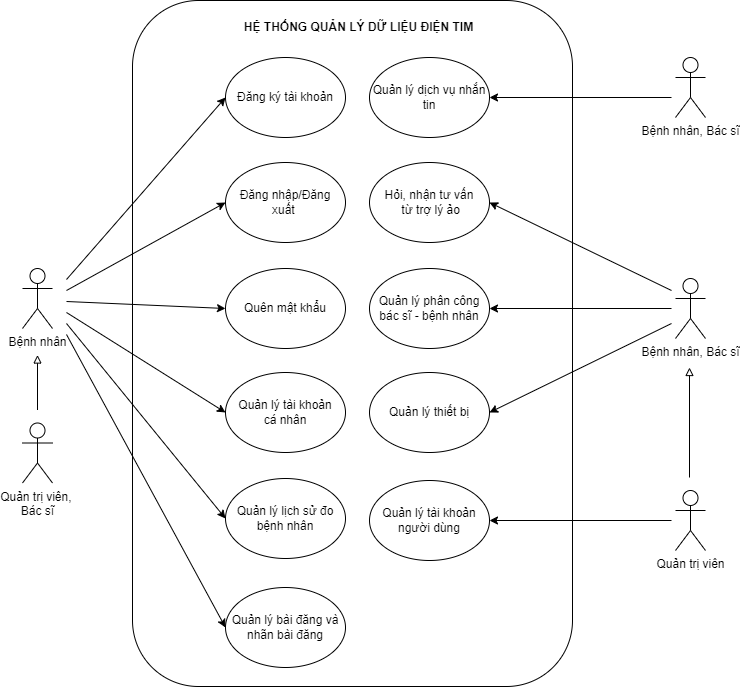
\includegraphics[width=16cm,height=14cm]{Images/use_case/use_case_general.png}
    \caption[Sơ đồ use case tổng quát của hệ thống]{\bfseries \fontsize{12pt}{0pt}
    \selectfont Sơ đồ use case tổng quát của hệ thống}
    \label{use_case_general} %đặt tên cho ảnh
  \end{figure}

\subsubsection{Use case chức năng xem lịch sử các lần đo}
  \begin{figure}[H]
    \centering
    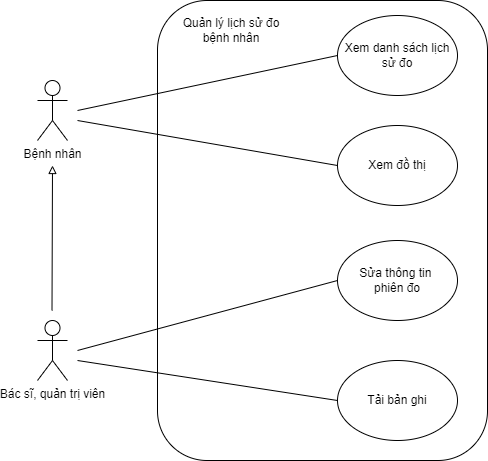
\includegraphics[width=12cm,height=4.8cm]{Images/use_case/use_case_view_history_record.png}
    \caption[Sơ đồ use case chức năng xem lịch sử các lần đo]{\bfseries \fontsize{12pt}{0pt}
    \selectfont Sơ đồ use case chức năng xem lịch sử các lần đo}
    \label{use_case_view_history_record} %đặt tên cho ảnh
  \end{figure}

  \begin{table}[H]
    \caption{\bfseries \fontsize{12pt}{0pt}\selectfont Bảng phân tích use case chức năng xem lịch sử các lần đo}
    \centering
    \begin{tabularx}{0.9\textwidth}{|c|X|}
      \hline
      \textbf{Tên chức năng} & \textbf{Xem lịch sử các lần đo} \\
      \hline
      Tác nhân & Bệnh nhân, Bác sĩ \\
      \hline
      Mô tả & Cho phép bệnh nhân xem lịch sử các lần đo điện tim và bác sĩ xem được lịch sử các lần đo của bệnh nhân
      mà mình quản lý \\
      \hline
      Điều kiện trước & Người dùng cần có kết nối Internet và đã đăng nhập \\
      \hline
      Dòng sự kiện chính & 
      % \begin{tabular}{@{}l@{}}
        Chi tiết luồng sự kiện được thể hiện ở Hình \ref{view_record_timeline}, Hình \ref{getEcgRecordsByUserId}, Hình \ref{getEcgRecordsByDoctor} 
        \\
      % \end{tabular} \\
      \hline
    \end{tabularx}
  \end{table}
% \newpage
\subsection{Thẻ CRC (Class - Responsibility - Collaboration Card)}

% \newpage
\subsection{Sơ đồ lớp}

% \newpage
\subsection{Sơ đồ tuần tự}
Để phân tích cụ thể hơn từng luồng trong hệ thống qua use case, chúng em xin phép được trình bày các sơ đồ tuần
tự. 
\subsubsection{Sơ đồ tuần tự chức năng đăng ký}
  \begin{figure}[H]
        \centering
        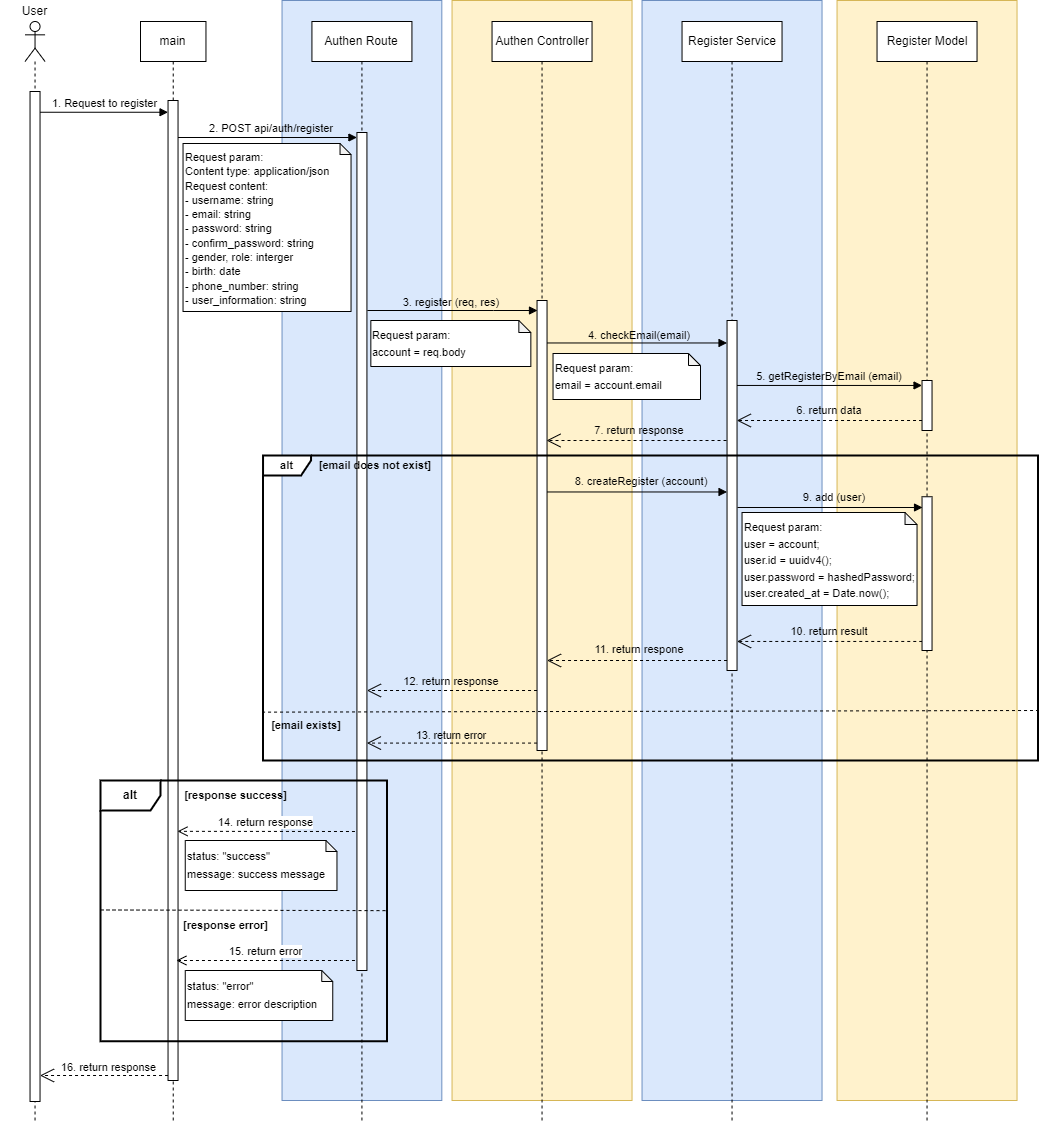
\includegraphics[width=12.9cm,height=9.4cm]{Images/mobile_app/register.png}
        \caption[Sơ đồ tuần tự chức năng đăng ký trên App]{\bfseries \fontsize{12pt}{0pt}
        \selectfont Sơ đồ tuần tự chức năng đăng ký trên App}
        \label{register} %đặt tên cho ảnh
  \end{figure}
  Sơ đồ tuần tự trên mô tả chi tiết quá trình người dùng đăng ký vào hệ thống. Người dùng gửi yêu cầu đăng ký, yêu cầu sẽ
  được xử lý bởi Control, nếu có lỗi phát sinh sẽ trả ra lỗi cho người dùng và yêu cầu người dùng nhập lại. Control
  sẽ xử lý cụ thể như thế nào được chúng em thể hiện trong Hình \ref{backend_register} trong chương sau.
\subsubsection{Sơ đồ tuần tự chức năng đăng nhập/đăng xuất}

    \begin{figure}[H]
         \centering
         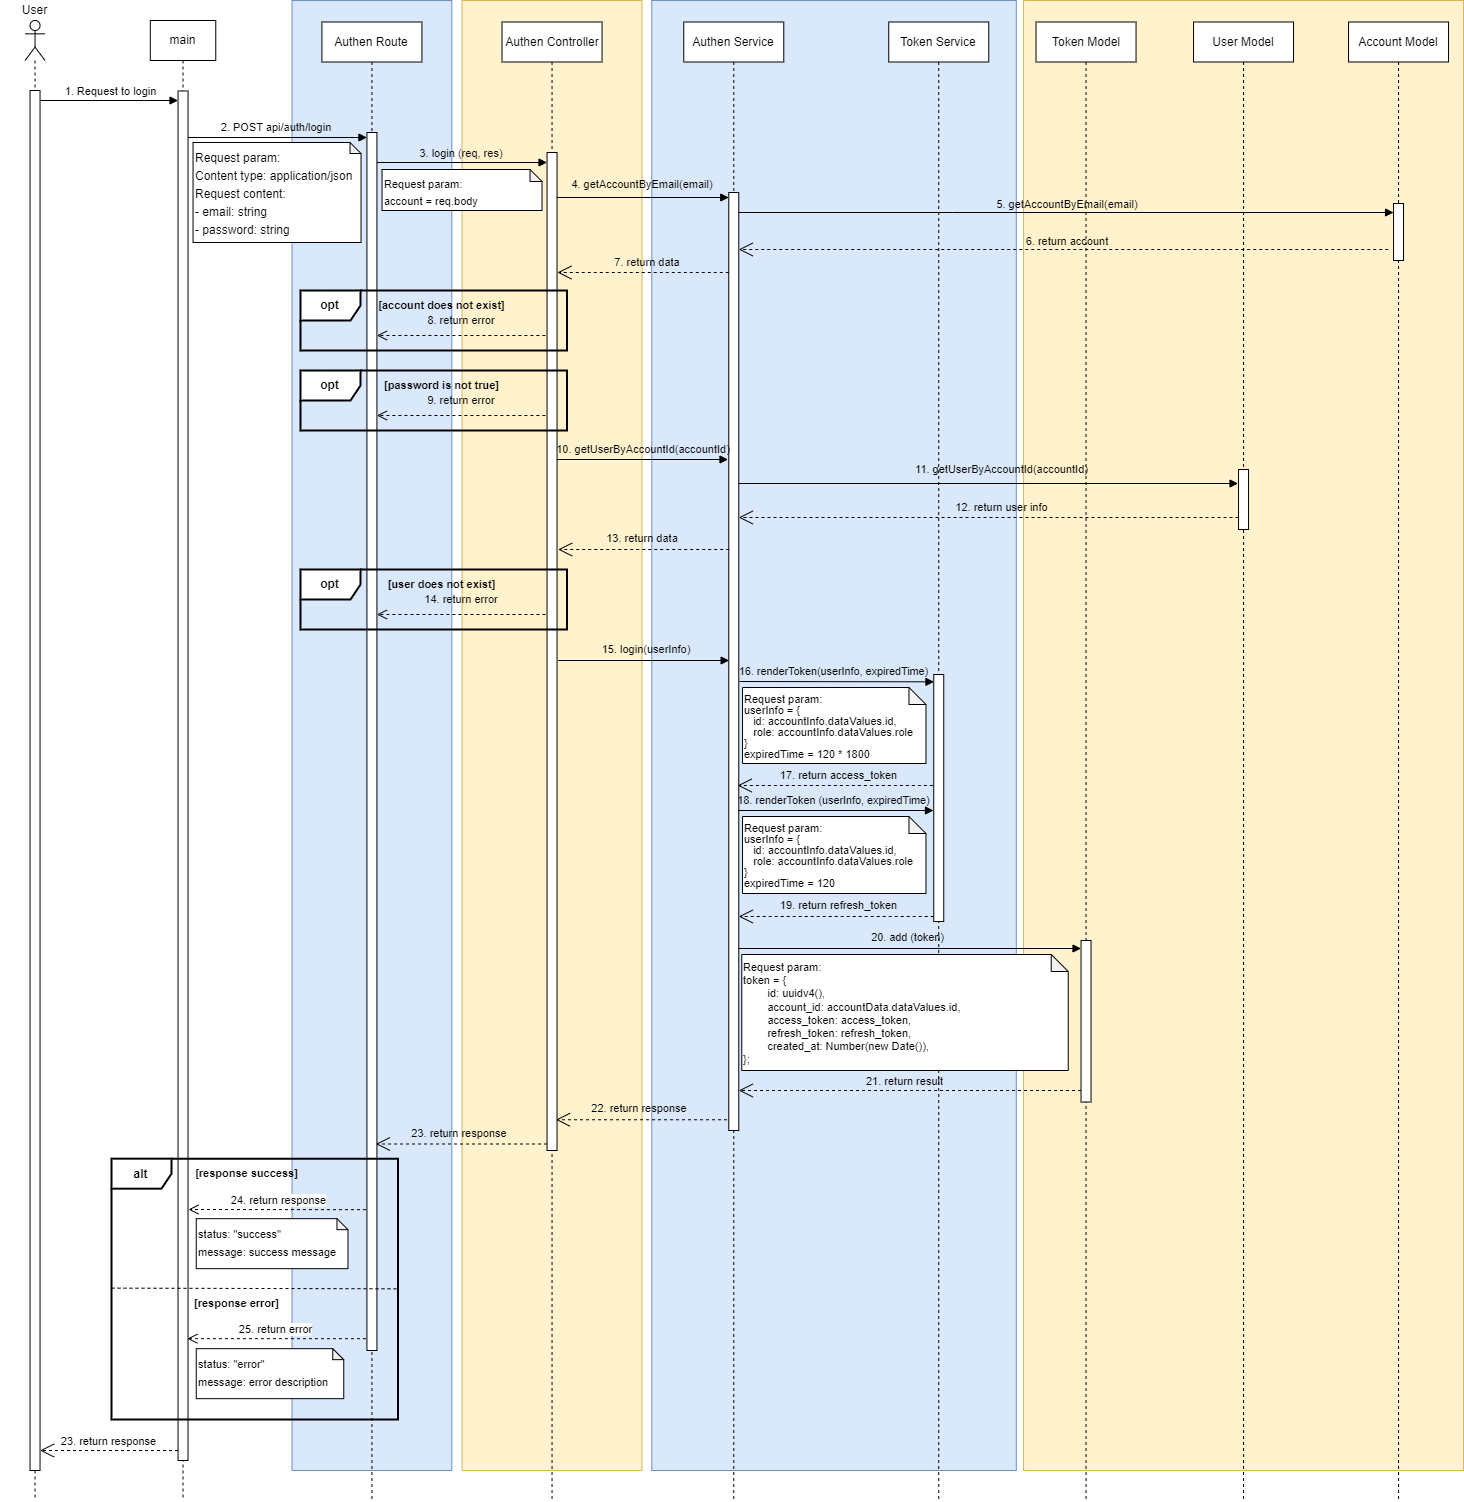
\includegraphics[width=16cm,height=12cm]{Images/mobile_app/login.png}
         \caption[Sơ đồ tuần tự chức năng đăng nhập trên App]{\bfseries \fontsize{12pt}{0pt}
         \selectfont Sơ đồ tuần tự chức năng đăng nhập trên App}
         \label{login} %đặt tên cho ảnh
    \end{figure}

  Sơ đồ tuần tự trên mô tả chi tiết quá trình người dùng đăng nhập vào hệ thống. Người dùng gửi yêu cầu đăng nhập, yêu cầu sẽ
  được xử lý bởi Control, nếu có lỗi phát sinh sẽ trả ra lỗi cho người dùng và yêu cầu người dùng nhập lại. Việc Control
  sẽ xử lý cụ thể yêu cầu người dùng được chúng em thể hiện trong Hình \ref{backend_login} trong chương sau.

  \begin{figure}[H]
    \centering
    \includegraphics[width=12cm,height=6cm]{Images/mobile_app/logout.png}
    \caption[Sơ đồ tuần tự chức năng đăng xuất trên App]{\bfseries \fontsize{12pt}{0pt}
    \selectfont Sơ đồ tuần tự chức năng đăng xuất trên App}
    \label{logout} %đặt tên cho ảnh
\end{figure}

Sơ đồ tuần tự trên mô tả chi tiết quá trình người dùng đăng xuất khỏi hệ thống. Người dùng gửi yêu cầu đăng xuất, yêu cầu sẽ
được xử lý bởi Control, nếu có lỗi phát sinh sẽ trả ra lỗi cho người dùng và yêu cầu người dùng nhập lại. Việc Control
sẽ xử lý cụ thể yêu cầu người dùng được chúng em thể hiện trong Hình \ref{backend_logout} trong chương sau.

\subsection{Phân tích dữ liệu}

Tại phần này, chúng em sẽ tiến hành xác định và mô tả các thực thể cũng như
 thuộc tính quan trọng trong hệ thống. Việc này giúp chúng ta có cái
  nhìn tổng quan về các yếu tố chính cần được quản lý và lưu trữ
   trong cơ sở dữ liệu. Bằng cách làm điều này, chúng ta có thể
    xây dựng một mô hình dữ liệu cơ bản để hỗ trợ việc thiết kế và
     triển khai hệ thống một cách hiệu quả.

     Trước hết, chúng em sẽ xác định và mô tả các thực thể chính trong hệ
      thống. Thực thể là các đối tượng hoặc khái niệm quan
       trọng mà chúng ta cần theo dõi và quản lý. Sau đó, chúng ta sẽ xác
        định các thuộc tính liên quan đến mỗi thực thể, các thông tin cần
         được lưu trữ và quản lý.

\begin{table}[H]
  \caption{\bfseries \fontsize{12pt}{0pt}\selectfont Bảng thực thể và thuộc tính}
  \centering
  \begin{tabularx}{0.9\textwidth}{|c|X|}
    \hline
    \textbf{Thực thể} & \textbf{Thuộc tính} \\
    \hline
    Người dùng & 
    ID người dùng, ID tài khoản, Tên người dùng, Email, Mật khẩu, Ngày sinh, Giới tính, Số điện thoại, Quyền, Thông tin người dùng \\
    \hline
    Token đăng nhập &
    ID token, ID tài khoản, Token truy cập, Token làm mới \\
    \hline
    Thiết bị & 
    ID thiết bị, ID người dùng thiết bị, ID bác sĩ theo dõi, Tên thiết bị, Loại thiết bị, Thông tin thiết bị, Trạng thái thiết bị, Ngày bắt đầu sử dụng\\
    \hline
    Các tần số đo được của thiết bị &
    ID tần số, ID thiết bị, Tên loại tần số, Thông tin, Giá trị đo được \\
    \hline
    Bản ghi ECG & 
    ID bản ghi ECG, ID người dùng, ID thiết bị, Loại bản ghi, Đường dẫn lưu trữ dữ liệu, Thời gian bắt đầu đo, Thời gian kết thúc đo \\
    \hline
    Thông tin đoạn hội thoại &
    ID đoạn hội thoại, Tên đoạn hội thoại, Loại đoạn hội thoại, Đường dẫn avatar đoạn hội thoại \\
    \hline
    Thành viên tham gia hội thoại &
    ID đoạn hội thoại, ID người dùng tham gia, Trạng thái thông báo (Có thông báo, Không thông báo), Tác vụ (người tạo đoạn hội thoại, thành viên trong đoạn hội thoại), Trạng thái đã xem\\
    \hline
    Tin nhắn & 
    ID tin nhắn, ID đoạn hội thoại, ID người gửi, Các tệp đính kèm, Tin nhắn hệ thống, Ghim (tin nhắn được ghim, không được ghim), Thời gian ghim tin nhắn, Các lượt thả cảm xúc \\
    \hline
    Tệp đính kèm &
    ID tệp đính kèm, ID tin nhắn, ID đoạn hội thoại, Đường dẫn nội dung, Tên tệp, Kích thước tệp, Đường dẫn thumbnail, Loại đính kèm (hình ảnh, video, tệp tin) \\
    \hline
    Hội thoại với AI &
    ID hội thoại, ID người gửi, Nội dung chat, Dữ liệu đầu vào \\
    \hline 
    Phân công bệnh nhân - bác sĩ & 
    ID phân công, ID bệnh nhân, ID bác sĩ, Ngày bắt đầu, Ngày kết thúc \\
    \hline
    Danh mục tin tức &
    ID danh mục tin tức, Tên danh mục tin tức, Mô tả danh mục tin tức \\
    \hline
    Tin tức &
    ID tin tức, Tiêu đề, Nội dung, ID danh mục tin tức, Tác giả, Đường dẫn, Đường dẫn hình ảnh \\
    \hline
  \end{tabularx}

  
\end{table}
Sau khi hoàn thành được bảng thực thể và thuộc tính, chúng em xác định được mô hình thực thể liên kết như sau:

\begin{figure}[H]
  \centering
  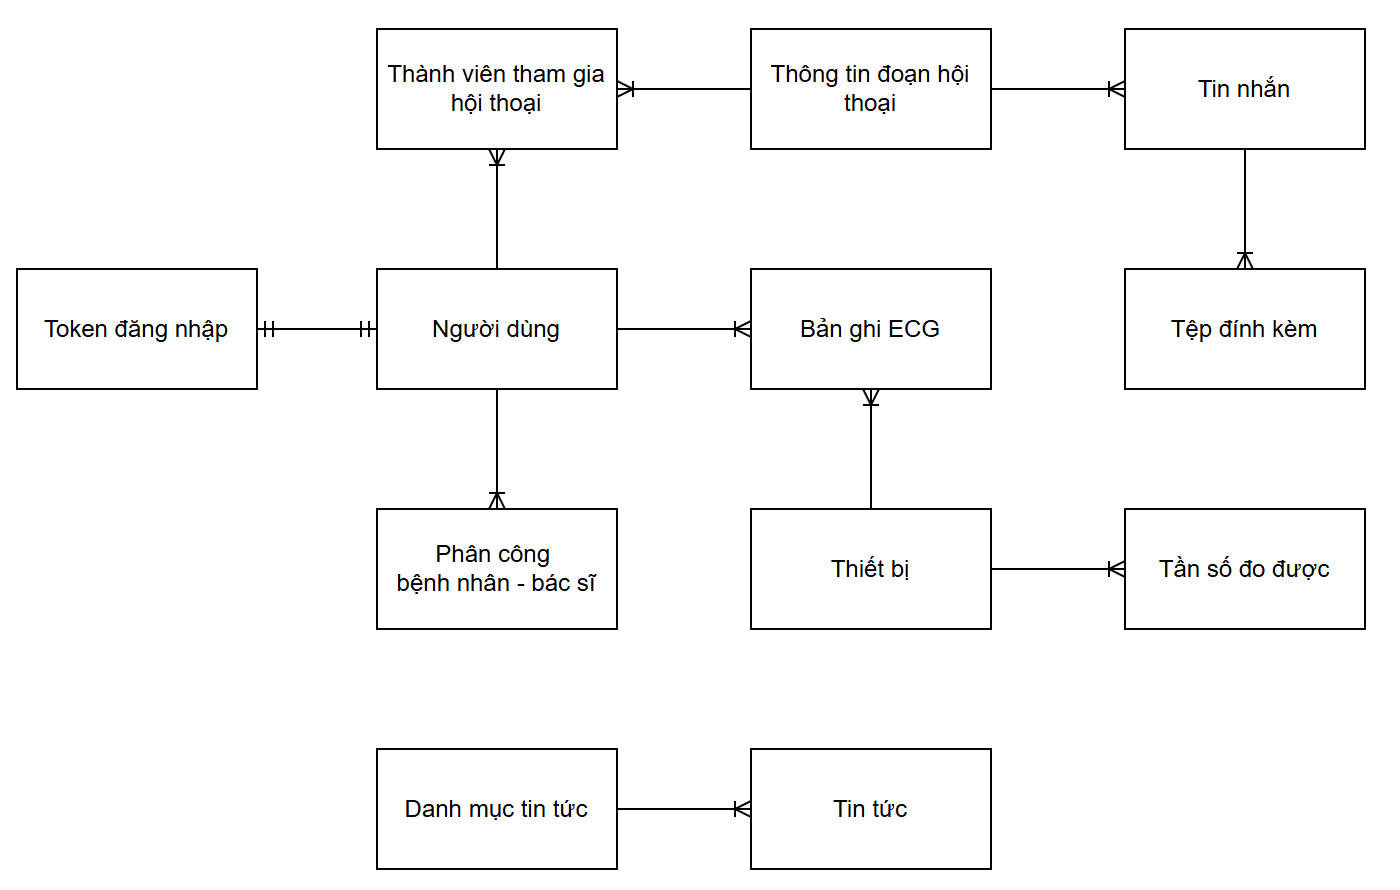
\includegraphics[width=15cm,height=8cm]{Images/system/fmECG_connection_entity.png}
  \caption[Mô hình thực thể liên kết]{\bfseries \fontsize{12pt}{0pt}
  \selectfont Mô hình thực thể liên kết}
  \label{ttlk} %đặt tên cho ảnh
\end{figure}

\subsection{Thiết kế cơ sở dữ liệu}
\subsubsection{Chuyển mô hình thực thể liên kết sang mô hình quan hệ}

\begin{itemize}
  \item Người dùng (\textbf{ID người dùng}, ID tài khoản, Tên người dùng, Email, Mật khẩu, Ngày sinh, Giới tính, Số điện thoại, Quyền, Thông tin người dùng)
  \item Token đăng nhập (\textbf{ID token}, ID tài khoản, Token truy cập, Token làm mới)
  \item Thiết bị (\textbf{ID thiết bị}, ID người dùng thiết bị, ID bác sĩ theo dõi, Tên thiết bị, Loại thiết bị, Thông tin thiết bị, Trạng thái thiết bị, Ngày bắt đầu sử dụng)
  \item Bản ghi ECG (\textbf{ID bản ghi ECG}, ID người dùng, ID thiết bị, Loại bản ghi, Đường dẫn lưu trữ dữ liệu, Thời gian bắt đầu đo, Thời gian kết thúc đo)
  \item Thông tin đoạn hội thoại (\textbf{ID đoạn hội thoại}, Tên đoạn hội thoại, Loại đoạn hội thoại, Đường dẫn avatar đoạn hội thoại)
  \item Thành viên tham gia hội thoại (\textbf{ID}, ID đoạn hội thoại, ID người dùng tham gia, Trạng thái thông báo, Tác vụ, Trạng thái đã xem)
  \item Tin nhắn (\textbf{ID tin nhắn}, ID đoạn hội thoại, ID người gửi, Các tệp đính kèm, Tin nhắn hệ thống, Ghim, Thời gian ghim tin nhắn, Các lượt thả cảm xúc)
  \item Tệp đính kèm (\textbf{ID tệp đính kèm}, ID tin nhắn, ID đoạn hội thoại, Đường dẫn nội dung, Tên tệp, Kích thước tệp, Đường dẫn thumbnail, Loại đính kèm)
  \item Hội thoại với AI (\textbf{ID hội thoại}, ID người gửi, Nội dung chat, Dữ liệu đầu vào)
  \item Phân công bệnh nhân - bác sĩ (\textbf{ID phân công}, ID bệnh nhân, ID bác sĩ, Ngày bắt đầu)
  \item Danh mục tin tức (\textbf{ID danh mục tin tức}, Tên danh mục tin tức, Mô tả danh mục tin tức)
  \item Tin tức (\textbf{ID tin tức}, Tiêu đề, Nội dung, ID danh mục tin tức, Tác giả, Đường dẫn, Đường dẫn hình ảnh)
\end{itemize}


\subsubsection{Chuẩn hoá 3NF}
Các bảng đã được thiết kế theo nguyên tắc chuẩn hoá 3NF, vì không có thuộc tính lặp lại và các thuộc tính không phụ thuộc vào một tập hợp con của khóa chính.

\paragraph{Chuẩn hoá bảng Người dùng}
\mbox{}

\begin{table}[H]
  \caption{\bfseries \fontsize{12pt}{0pt}\selectfont Bảng chuẩn hoá bảng Người dùng}
  \centering
  \begin{tabularx}{0.9\textwidth}{|X|X|}
    \hline
    \textbf{Danh sách thuộc tính} & ID người dùng, ID tài khoản, Tên người dùng, Email, Mật khẩu, Ngày sinh, Giới tính, Số điện thoại, Quyền, Thông tin người dùng \\
    \hline
    \textbf{Quy tắc nghiệp vụ} & \textbf{Phụ thuộc hàm} \\
    \hline
    Mỗi người dùng có một ID riêng, có duy nhất mật khẩu, email, tên, ngày sinh, số điện thoại, quyền,
    giới tính, thông tin & \parbox[t]{\linewidth}{$\text{ID người dùng} \rightarrow$ mật khẩu, email, tên, ngày sinh, số điện thoại, quyền, thông tin} \\
    \hline
    \multicolumn{2}{|X|}{$\Rightarrow \text{Khoá chính của bảng: ID người dùng}$} \\
    \multicolumn{2}{|X|}{$\Rightarrow \text{Bảng Người dùng đã ở 3NF}$} \\
    \hline
  \end{tabularx}
\end{table}

\paragraph{Chuẩn hoá bảng Token đăng nhập}
\mbox{}

\begin{table}[H]
  \caption{\bfseries \fontsize{12pt}{0pt}\selectfont Bảng chuẩn hoá bảng Token đăng nhập}
  \centering
  \begin{tabularx}{0.9\textwidth}{|X|X|}
    \hline
    \textbf{Danh sách thuộc tính} & ID token, ID tài khoản, Token truy cập, Token làm mới \\
    \hline
    \textbf{Quy tắc nghiệp vụ} & \textbf{Phụ thuộc hàm} \\
    \hline
    Mỗi người dùng có một ID token riêng, có duy nhất ID tài khoản, token truy cập và token làm mới 
    & \parbox[t]{\linewidth}{$\text{ID token} \rightarrow$ ID tài khoản, Token truy cập, Token làm mới} \\
    \hline
    \multicolumn{2}{|X|}{$\Rightarrow \text{Khoá chính của bảng: ID token đăng nhập}$} \\
    \multicolumn{2}{|X|}{$\Rightarrow \text{Bảng Token  đã ở 3NF}$} \\
    \hline
  \end{tabularx}
\end{table}

\paragraph{Chuẩn hoá bảng Thiết bị}
\mbox{}

\begin{table}[H]
  \caption{\bfseries \fontsize{12pt}{0pt}\selectfont Bảng chuẩn hoá bảng Thiết bị}
  \centering
  \begin{tabularx}{0.9\textwidth}{|X|X|}
    \hline
    \textbf{Danh sách thuộc tính} & ID thiết bị, ID người dùng thiết bị, ID bác sĩ theo dõi, Tên thiết bị, 
    Loại thiết bị, Thông tin thiết bị, Trạng thái thiết bị, Ngày bắt đầu sử dụng \\
    \hline
    \textbf{Quy tắc nghiệp vụ} & \textbf{Phụ thuộc hàm} \\
    \hline
    Mỗi thiết bị khi được sử dụng sẽ có một ID thiết bị riêng, có duy nhất tên thiết bị, loại thiết bị, thông tin thiết bị.
    ID người dùng thiết bị, ID bác sĩ theo dõi, trạng thái thiết bị, ngày bắt đầu sử dụng
    & \parbox[t]{\linewidth}{$\text{ID thiết bị} \rightarrow$ ID người dùng thiết bị, ID bác sĩ theo dõi, Tên thiết bị, 
    Loại thiết bị, Thông tin thiết bị, Trạng thái thiết bị, Ngày bắt đầu sử dụng} \\
    \hline
    \multicolumn{2}{|X|}{$\Rightarrow \text{Khoá chính của bảng: ID thiết bị}$} \\
    \multicolumn{2}{|X|}{$\Rightarrow \text{Bảng Thiết bị đã ở 3NF}$} \\
    \hline
  \end{tabularx}
\end{table}

\paragraph{Chuẩn hoá bảng Bản ghi ECG}
\mbox{}

\begin{table}[H]
  \caption{\bfseries \fontsize{12pt}{0pt}\selectfont Bảng chuẩn hoá bảng Bản ghi ECG}
  \centering
  \begin{tabularx}{0.9\textwidth}{|X|X|}
    \hline
    \textbf{Danh sách thuộc tính} & ID bản ghi ECG, ID người dùng, ID thiết bị, Loại bản ghi, 
    Đường dẫn lưu trữ dữ liệu, Thời gian bắt đầu đo, Thời gian kết thúc đo \\
    \hline
    \textbf{Quy tắc nghiệp vụ} & \textbf{Phụ thuộc hàm} \\
    \hline
    Mỗi bản ghi có một ID bản ghi ECG riêng, có duy nhất ID người dùng, ID thiết bị, Loại bản ghi, 
    Đường dẫn lưu trữ dữ liệu, Thời gian bắt đầu đo, Thời gian kết thúc đo
    & \parbox[t]{\linewidth}{$\text{ID bản ghi ECG} \rightarrow$ ID người dùng, ID thiết bị, Loại bản ghi, 
    Đường dẫn lưu trữ dữ liệu, Thời gian bắt đầu đo, Thời gian kết thúc đo} \\
    \hline
    \multicolumn{2}{|X|}{$\Rightarrow \text{Khoá chính của bảng: ID bản ghi ECG}$} \\
    \multicolumn{2}{|X|}{$\Rightarrow \text{Bảng Bản ghi ECG đã ở 3NF}$} \\
    \hline
  \end{tabularx}
\end{table}

\paragraph{Chuẩn hoá bảng Thông tin đoạn hội thoại}
\mbox{}

\begin{table}[H]
  \caption{\bfseries \fontsize{12pt}{0pt}\selectfont Bảng chuẩn hoá bảng Thông tin đoạn hội thoại}
  \centering
  \begin{tabularx}{0.9\textwidth}{|X|X|}
    \hline
    \textbf{Danh sách thuộc tính} & ID đoạn hội thoại, Tên đoạn hội thoại, 
    Loại đoạn hội thoại, Đường dẫn avatar đoạn hội thoại \\
    \hline
    \textbf{Quy tắc nghiệp vụ} & \textbf{Phụ thuộc hàm} \\
    \hline
    Mỗi đoạn hội thoại có một ID đoạn hội thoại riêng, có duy nhất tên đoạn hội thoại, 
    loại đoạn hội thoại, đường dẫn avatar đoạn hội thoại
    & \parbox[t]{\linewidth}{$\text{ID đoạn hội thoại} \rightarrow$ Tên đoạn hội thoại, 
    Loại đoạn hội thoại, Đường dẫn avatar đoạn hội thoại} \\
    \hline
    \multicolumn{2}{|X|}{$\Rightarrow \text{Khoá chính của bảng: ID đoạn hội thoại}$} \\
    \multicolumn{2}{|X|}{$\Rightarrow \text{Bảng Thông tin đoạn hội thoại đã ở 3NF}$} \\
    \hline
  \end{tabularx}
\end{table}

\paragraph{Chuẩn hoá bảng Thành viên tham gia hội thoại}
\mbox{}

\begin{table}[H]
  \caption{\bfseries \fontsize{12pt}{0pt}\selectfont Bảng chuẩn hoá bảng Thành viên tham gia hội thoại}
  \centering
  \begin{tabularx}{0.9\textwidth}{|X|X|}
    \hline
    \textbf{Danh sách thuộc tính} & ID, ID đoạn hội thoại, ID người dùng tham gia,
    Trạng thái thông báo, Tác vụ, Trạng thái đã xem \\
    \hline
    \textbf{Quy tắc nghiệp vụ} & \textbf{Phụ thuộc hàm} \\
    \hline
    Mỗi đoạn hội thoại có nhiều ID người dùng tham gia, mỗi người dùng có duy nhất trạng thái thông báo,
    tác vụ, trạng thái đã xem trong một đoạn hội thoại
    & \parbox[t]{\linewidth}{$\text{ID} \rightarrow$ ID đoạn hội thoại, ID người dùng tham gia,
    Trạng thái thông báo, Tác vụ, Trạng thái đã xem} \\
    \hline
    \multicolumn{2}{|X|}{$\Rightarrow \text{Khoá chính của bảng: ID}$} \\
    \multicolumn{2}{|X|}{$\Rightarrow \text{Bảng Thành viên tham gia hội thoại đã ở 3NF}$} \\
    \hline
  \end{tabularx}
\end{table}

\paragraph{Chuẩn hoá bảng Tin nhắn}
\mbox{}

\begin{table}[H]
  \caption{\bfseries \fontsize{12pt}{0pt}\selectfont Bảng chuẩn hoá bảng Tin nhắn}
  \centering
  \begin{tabularx}{0.9\textwidth}{|X|X|}
    \hline
    \textbf{Danh sách thuộc tính} & ID tin nhắn, ID đoạn hội thoại, ID người gửi, Các tệp đính kèm, 
    Tin nhắn hệ thống, Ghim, Thời gian ghim tin nhắn, Các lượt thả cảm xúc \\
    \hline
    \textbf{Quy tắc nghiệp vụ} & \textbf{Phụ thuộc hàm} \\
    \hline
    Mỗi tin nhắn có một ID tin nhắn riêng, thuộc một đoạn hội thoại, có duy nhất ID người gửi, các tệp đính kèm,
    tin nhắn hệ thống, ghim, thời gian ghim tin nhắn, các lượt thả cảm xúc
    & \parbox[t]{\linewidth}{$\text{ID tin nhắn} \rightarrow$ ID đoạn hội thoại, ID người gửi, các tệp đính kèm,
    tin nhắn hệ thống, ghim, thời gian ghim tin nhắn, các lượt thả cảm xúc} \\
    \hline
    \multicolumn{2}{|X|}{$\Rightarrow \text{Khoá chính của bảng: ID tin nhắn}$} \\
    \multicolumn{2}{|X|}{$\Rightarrow \text{Bảng Tin nhắn đã ở 3NF}$} \\
    \hline
  \end{tabularx}
\end{table}

\paragraph{Chuẩn hoá bảng Tệp đính kèm}
\mbox{}

\begin{table}[H]
  \caption{\bfseries \fontsize{12pt}{0pt}\selectfont Bảng chuẩn hoá bảng Tệp đính kèm}
  \centering
  \begin{tabularx}{0.9\textwidth}{|X|X|}
    \hline
    \textbf{Danh sách thuộc tính} & ID tệp đính kèm, ID tin nhắn, ID đoạn hội thoại, Đường dẫn nội
    dung, Tên tệp, Kích thước tệp, Đường dẫn thumbnail, Loại đính kèm \\
    \hline
    \textbf{Quy tắc nghiệp vụ} & \textbf{Phụ thuộc hàm} \\
    \hline
    Mỗi tệp đính kèm có một ID tệp đính kèm riêng, thuộc một tin nhắn trong một đoạn hội thoại, có duy nhất đường dẫn nội
    dung, tên tệp, kích thước tệp, đường dẫn thumbnail, loại đính kèm
    & \parbox[t]{\linewidth}{$\text{ID tệp đính kèm} \rightarrow$ ID tin nhắn, ID đoạn hội thoại, Đường dẫn nội
    dung, Tên tệp, Kích thước tệp, Đường dẫn thumbnail, Loại đính kèm} \\
    \hline
    \multicolumn{2}{|X|}{$\Rightarrow \text{Khoá chính của bảng: ID tệp đính kèm}$} \\
    \multicolumn{2}{|X|}{$\Rightarrow \text{Bảng Tệp đính kèm đã ở 3NF}$} \\
    \hline
  \end{tabularx}
\end{table}

\paragraph{Chuẩn hoá bảng Phân công bệnh nhân - bác sĩ}
\mbox{}

\begin{table}[H]
  \caption{\bfseries \fontsize{12pt}{0pt}\selectfont Bảng chuẩn hoá bảng Phân công bệnh nhân - bác sĩ}
  \centering
  \begin{tabularx}{0.9\textwidth}{|X|X|}
    \hline
    \textbf{Danh sách thuộc tính} & ID phân công, ID bệnh nhân, ID bác sĩ, Ngày bắt đầu \\
    \hline
    \textbf{Quy tắc nghiệp vụ} & \textbf{Phụ thuộc hàm} \\
    \hline
    Mỗi phân công bệnh nhân - bác sĩ có một ID phân công riêng, có duy nhất ID bệnh nhân, ID bác sĩ, ngày bắt đầu.
    Mỗi bệnh nhân thuộc một phân công duy nhất, còn mỗi bác sĩ có thể được giao nhiều phân công.
    & \parbox[t]{\linewidth}{$\text{ID phân công} \rightarrow$ ID bệnh nhân, ID bác sĩ, Ngày bắt đầu} \\
    \hline
    \multicolumn{2}{|X|}{$\Rightarrow \text{Khoá chính của bảng: ID phân công}$} \\
    \multicolumn{2}{|X|}{$\Rightarrow \text{Bảng Phân công bệnh nhân - bác sĩ đã ở 3NF}$} \\
    \hline
  \end{tabularx}
\end{table}

\paragraph{Chuẩn hoá bảng Danh mục tin tức}
\mbox{}

\begin{table}[H]
  \caption{\bfseries \fontsize{12pt}{0pt}\selectfont Bảng chuẩn hoá bảng Danh mục tin tức}
  \centering
  \begin{tabularx}{0.9\textwidth}{|X|X|}
    \hline
    \textbf{Danh sách thuộc tính} & ID danh mục tin tức, Tên danh mục tin tức, Mô tả danh mục tin tức \\
    \hline
    \textbf{Quy tắc nghiệp vụ} & \textbf{Phụ thuộc hàm} \\
    \hline
    Mỗi danh mục tin tức có một ID danh mục tin tức riêng, có duy nhất tên danh mục tin tức, mô tả danh mục tin tức
    & \parbox[t]{\linewidth}{$\text{ID danh mục tin tức} \rightarrow$ Tên danh mục tin tức, Mô tả danh mục tin tức} \\
    \hline
    \multicolumn{2}{|X|}{$\Rightarrow \text{Khoá chính của bảng: ID danh mục tin tức}$} \\
    \multicolumn{2}{|X|}{$\Rightarrow \text{Bảng Danh mục tin tức đã ở 3NF}$} \\
    \hline
  \end{tabularx}
\end{table}

\paragraph{Chuẩn hoá bảng Tin tức}
\mbox{}

\begin{table}[H]
  \caption{\bfseries \fontsize{12pt}{0pt}\selectfont Bảng chuẩn hoá bảng Tin tức}
  \centering
  \begin{tabularx}{0.9\textwidth}{|X|X|}
    \hline
    \textbf{Danh sách thuộc tính} & ID tin tức, Tiêu đề, Nội dung, ID danh mục tin tức, Tác giả, Đường dẫn,
    Đường dẫn hình ảnh \\
    \hline
    \textbf{Quy tắc nghiệp vụ} & \textbf{Phụ thuộc hàm} \\
    \hline
    Mỗi tin tức có một ID tin tức riêng, thuộc duy nhất một danh mục tin tức, có duy nhất tiêu đề, 
    nội dung, tác giả, đường dẫn, đường dẫn hình ảnh
    & \parbox[t]{\linewidth}{$\text{ID tin tức} \rightarrow$ Tiêu đề, Nội dung, ID danh mục tin tức, Tác giả, 
    Đường dẫn, Đường dẫn hình ảnh} \\
    \hline
    \multicolumn{2}{|X|}{$\Rightarrow \text{Khoá chính của bảng: ID tin tức}$} \\
    \multicolumn{2}{|X|}{$\Rightarrow \text{Bảng Tin tức đã ở 3NF}$} \\
    \hline
  \end{tabularx}
\end{table}

\subsection{Kết luận chương}

Trong chương này, chúng em đã thực hiện phân tích toàn diện về
 hệ thống cho đề tài , nhằm đáp ứng
  các mục tiêu và yêu cầu đã được đề xuất.

Chúng em đã xác định rõ ràng các khía cạnh quan trọng của hệ thống,
 tập trung vào việc thiết kế một hệ thống quản lý ECG hiệu quả,
  trực quan và có khả năng theo dõi sức khỏe tim mạch một cách
   chính xác. 


\newpage


\section*{CHƯƠNG 3. THIẾT KẾ HỆ THỐNG}
\setcounter{section}{3}
\setcounter{subsection}{0} %LƯU Ý MỖI LẦN THÊM CHƯƠNG MỚI CẦN THÊM CÂU NÀY ĐỂ RESET THỨ TỰ CỦA SUBSECTON VỀ 1
\setcounter{table}{0} % LƯU Ý SAU MỖI LẦN GỌI BẢNG HAY HÌNH ẢNH PHẢI THÊM CÂU NÀY ĐỂ RESET THỨ TỰ
\setcounter{figure}{0} %% LƯU Ý SAU MỖI LẦN GỌI BẢNG HAY HÌNH ẢNH PHẢI THÊM CÂU NÀY ĐỂ RESET THỨ TỰ
\addcontentsline{toc}{section}{\numberline{}CHƯƠNG 3. THIẾT KẾ HỆ THỐNG}

Trong chương này, chúng em sẽ trình bày về thiết kế hệ thống từ tổng quan đến chi tiết dựa trên phân tích từ Chương 2.
Đầu tiên là xây dựng sơ đồ kiến trúc hệ thống.
Sau đó thiết kế giao diện, chức năng cho website và server.
Nội dung chính của chương tập trung vào các hình ảnh và sơ đồ mô tả từng luồng hoạt động của hệ thống.
\subsection{Sơ đồ kiến trúc tổng quan của hệ thống}

\begin{figure}[H]
  \centering
  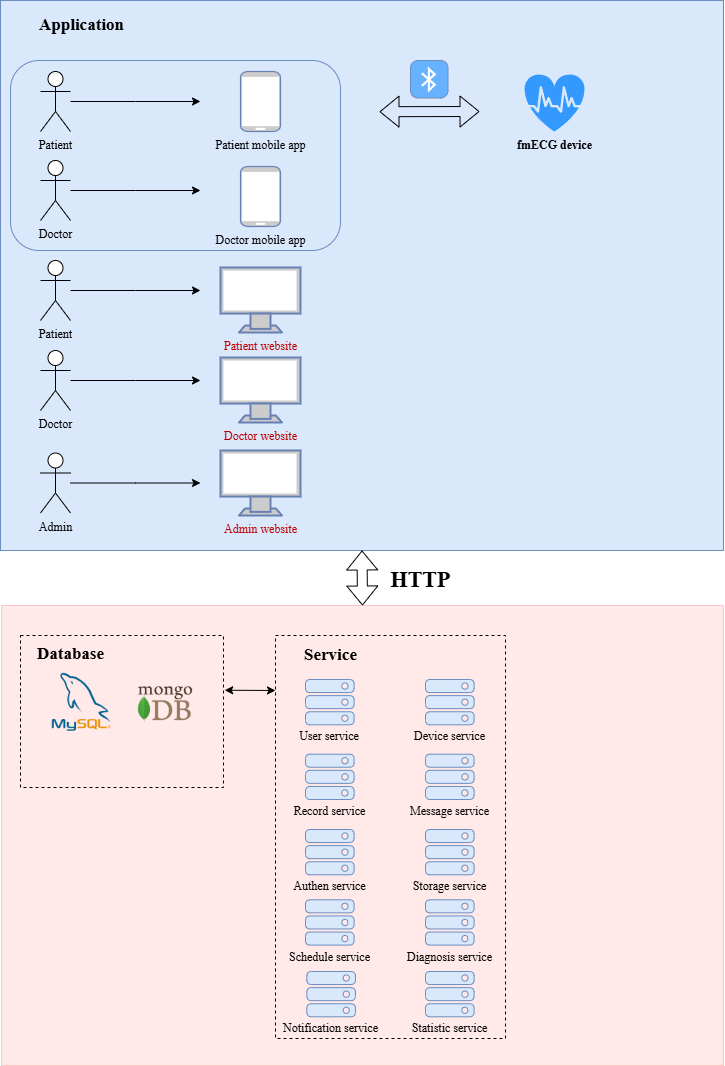
\includegraphics[width=12cm,height=18cm]{Images/System/fmECG_architecture-System_Architecture.drawio.png}
  \caption[Kiến trúc tổng quan hệ thống]{\bfseries \fontsize{12pt}{0pt}\selectfont Kiến trúc tổng quan hệ thống}
  \label{fmECG_architecture-System} %đặt tên cho ảnh
\end{figure}
Hệ thống được chia làm ba phần chính bao gồm Device (Thiết bị), Server (Máy chủ) và Application (Ứng dụng bao gồm: web và app).
Mỗi thành phần đóng vai trò quan trọng trong việc vận hành tổng thể hệ thống trong hình vẽ

Hình \ref{fmECG_architecture-System} thể hiện ba phần: 

\begin{adjustwidth}{1.5em}{}
\begin{itemize}
  \item Device (Thiết bị): Bao gồm thiết bị phần cứng đo điện tim, có thể kết nối với ứng dụng di động của bệnh nhân thông qua Bluetooth.
  \item Application (Ứng dụng): Bao gồm ứng dụng di động và website cho bệnh nhân, bác sĩ, quản trị viên.
  \item Server (Máy chủ): Bao gồm các Services để xử lý các yêu cầu gửi từ Application, cơ sở dữ liệu.
\end{itemize}
\end{adjustwidth}

Hệ thống được thiết kế với sự tương tác trực tiếp giữa bệnh nhân và thiết bị thông qua ứng dụng di động. 
Ứng dụng đóng vai trò trung gian, giao tiếp với máy chủ bằng API và giao thức HTTP. 
Máy chủ chịu trách nhiệm xử lý dữ liệu thông qua các dịch vụ chuyên biệt. 
Mỗi dịch vụ được thiết kế để xử lý một loại yêu cầu cụ thể, bao gồm cả việc truy vấn và cập nhật cơ sở dữ liệu, 
trước khi trả kết quả về cho người dùng.\begin{adjustwidth}{1.5em}{}
\begin{itemize}
  \item User service: Xử lý các yêu cầu liên quan đến người dùng như đăng ký, đăng nhập, lấy thông tin cá nhân
  \item Device service: Xử lý các tác vụ liên quan tới thiết bị như thêm, sửa, xoá thiết bị, cập nhật thông tin.
  \item Storage service: Xử lý các tác vụ liên quan tới lưu trữ dữ liệu của hệ thống.
  \item Record service: Xử lý các tác vụ liên quan tới bản ghi như thêm, sửa, xoá, xử lý dữ liệu file đo.
  \item Message service: Xử lý các yêu cầu liên quan tới tin nhắn.
  \item Authen service: Xử lý các tác vụ liên quan tới bảo mật như: mã hoá và cung cấp token, kiểm tra token, phân quyền truy cập api, mã hoá các dữ liệu nhạy cảm trước khi lưu trữ.
  \item Statistic service: Xử lý các tác vụ liên quan tới thống kê như: thống kê người dùng, thiết bị, bản ghi.
  \item Schedule service: Xử lý các tác vụ liên quan đến đặt lịch hẹn, phản hồi lịch.
\end{itemize}
\end{adjustwidth}

Sau đây là mô tả chi tiết về từng khối nhỏ hơn trong kiến trúc hệ thống, dựa trên các đối tượng đã được xác định trong hệ thống.
\newpage
\subsection{Sơ đồ khối phần mềm}

\subsubsection{Ứng dụng di động dành cho bệnh nhân}
\begin{figure}[H]
  \centering
  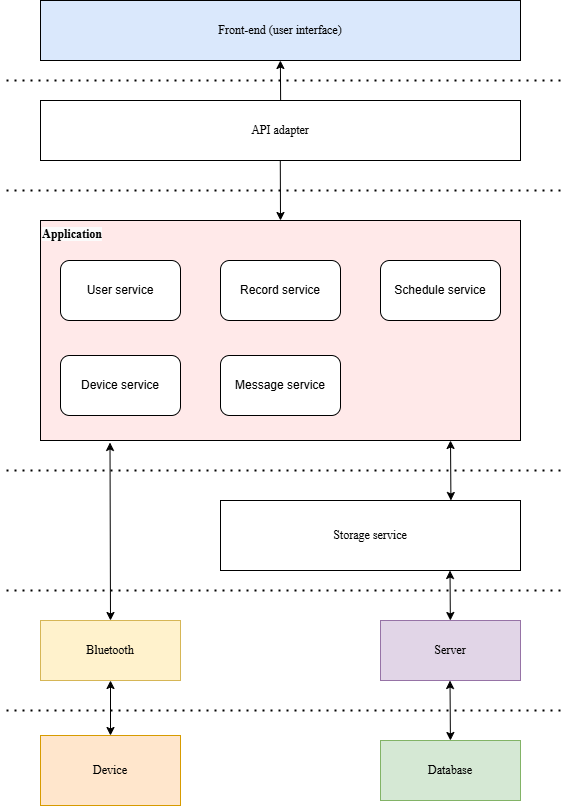
\includegraphics[width=12cm,height=14cm]{Images/System/fmECG_architecture-Patient-App.drawio.png}
  \caption[Sơ đồ khối ứng dụng di động dành cho bệnh nhân]{\bfseries \fontsize{12pt}{0pt}\selectfont Sơ đồ khối ứng dụng di động dành cho bệnh nhân}
  \label{fmECG_architecture-Patient-App} %đặt tên cho ảnh
\end{figure}
% Lớp trên cùng trong sơ đồ hình \ref{fmECG_architecture-Patient} là lớp giao diện người dùng,
% nơi người dùng trực tiếp tương tác với hệ thống, thực hiện các request thông qua API Adapter.

% Sau đó các request được gửi đến lớp Application nơi chứa các Services để xử lý các request từ người dùng. 
% Kết quả được trả về giao diện. Ở đây các services gồm có: 

% \begin{adjustwidth}{1.5em}{}
%   \begin{itemize}
%     \item User service: Khối có nhiệm vụ xử lý thông tin cá nhân
%     \item Device service: Khối có nhiệm vụ xử lý các vấn đề liên quan đến mượn trả thiết bị.
%     \item Schedule service: Khối có nhiệm vụ quản lý việc đặt lịch của bệnh nhân
%     \item Record service: Khối có nhiệm vụ xử lý thông tin bản ghi
%     \item Message service: Khối có nhiệm vụ quản lý việc chat, trao đổi thông tin với bác sĩ
%     \item Storage service: Khối service đặc biệt có nhiệm vụ lưu thông tin vào bộ nhớ
%   \end{itemize}
% \end{adjustwidth}
Tầng trên cùng trong sơ đồ hình \ref{fmECG_architecture-Patient-App} là User Interface (Giao diện người dùng), nơi bệnh nhân trực tiếp tương tác với hệ thống thông qua API Adapter để gửi yêu cầu và nhận phản hồi.
Các yêu cầu này được xử lý bởi các Services chính, bao gồm User Service, Device Service, Record Service, Schedule Service, Diagnosis Service, Notification Service và Storage Service.

Những Services này được thiết kế nhằm đáp ứng các nhu cầu của bệnh nhân, từ quản lý thông tin cá nhân, mượn và trả thiết bị, theo dõi lịch sử dữ liệu phiên đo, cho đến việc quản lý lịch khám,
tra cứu thông tin chẩn đoán cho từng lịch khám. Ngoài ra, hệ thống còn đảm bảo việc gửi thông báo nhắc nhở kịp thời và hỗ trợ bệnh nhân trao đổi thông tin với bác sĩ một cách liền mạch và hiệu quả.

\subsubsection{Ứng dụng di động dành cho bác sĩ}
\begin{figure}[H]
  \centering
  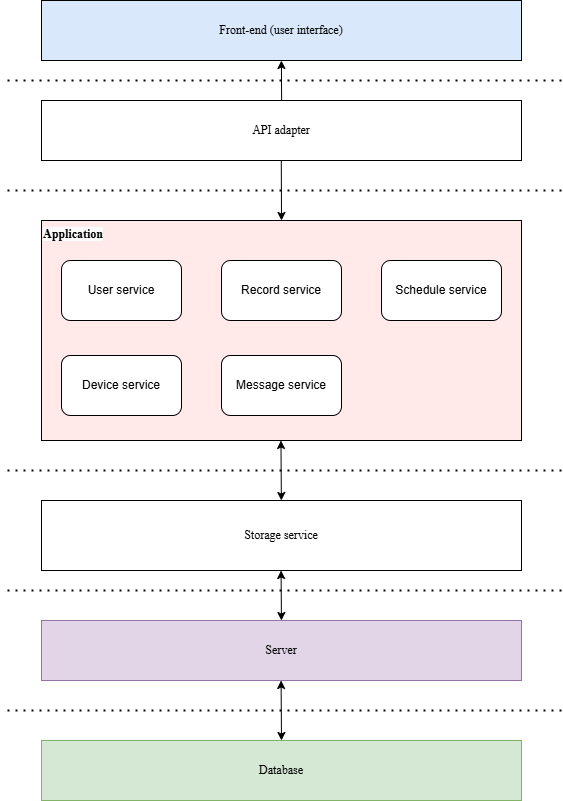
\includegraphics[width=12cm,height=14cm]{Images/System/fmECG_architecture-Doctors.drawio.png}
  \caption[Sơ đồ khối Ứng dụng dành cho bác sĩ]{\bfseries \fontsize{12pt}{0pt}\selectfont Sơ đồ khối ứng dụng di động dành cho bác sĩ}
  \label{fmECG_architecture-Doctor} %đặt tên cho ảnh
\end{figure}
% \begin{adjustwidth}{1.5em}{}
%   \begin{itemize}
%     \item User service: Khối có nhiệm vụ xử lý thông tin cá nhân
%     \item Device service: Khối có nhiệm vụ xử lý các vấn đề liên quan đến mượn trả thiết bị.
%     \item Schedule service: Khối có nhiệm vụ quản lý việc đặt lịch của bệnh nhân
%     \item Record service: Khối có nhiệm vụ xử lý thông tin bản ghi
%     \item Message service: Khối có nhiệm vụ quản lý việc chat, trao đổi thông tin với bác sĩ,
%     trao đổi trong nhóm.
%     \item Storage service: Khối service đặc biệt có nhiệm vụ lưu thông tin vào bộ nhớ
%   \end{itemize}
% \end{adjustwidth}
Tương tự với bệnh nhân, sơ đồ hình \ref{fmECG_architecture-Doctor} được xây dựng để hỗ trợ bác sĩ thực hiện các nhiệm vụ chuyên môn thông qua giao diện người dùng và API Adapter, đảm bảo việc xử lý thông tin diễn ra nhanh chóng và hiệu quả.

Các Services chính, bao gồm User Service, Device Service, Record Service, Schedule Service, Diagnosis Service, Notification Service và Storage Service, đóng vai trò quan trọng trong việc hỗ trợ bác sĩ.
Các nhiệm vụ được tập trung vào việc theo dõi và phân tích dữ liệu phiên đo từ bệnh nhân, quản lý lịch khám, chấp nhận hoặc từ chối yêu cầu đặt lịch, ghi nhận thông tin chẩn đoán, và trao đổi trực tiếp với bệnh nhân.
Hơn nữa, hệ thống cung cấp khả năng tự động gửi thông báo về lịch khám và nhắc nhở các cuộc khám sắp tới, giúp bác sĩ quản lý thời gian và công việc hiệu quả hơn.

Cách tiếp cận này không chỉ hỗ trợ bác sĩ tổ chức công việc thuận lợi mà còn góp phần nâng cao hiệu quả điều trị cho bệnh nhân.

\subsubsection{Website cho quản trị viên}
\begin{figure}[H]
  \centering
  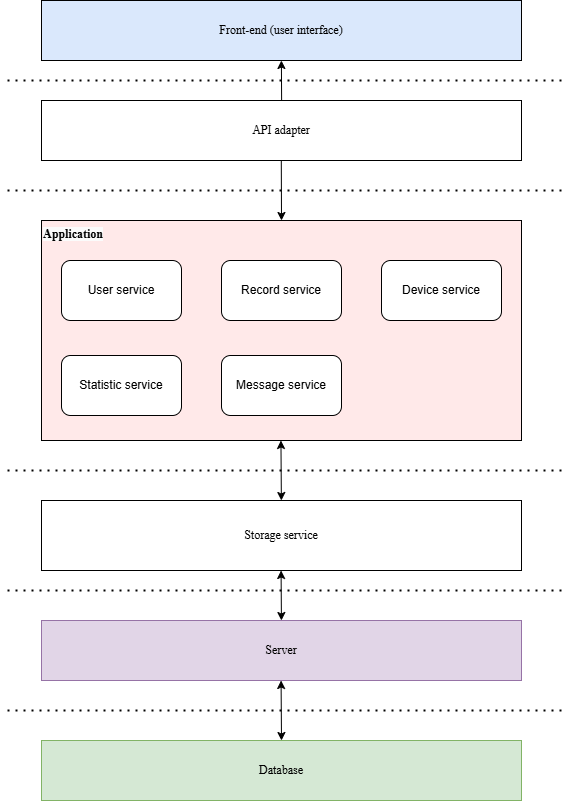
\includegraphics[width=12cm,height=14cm]{Images/System/fmECG_architecture-Admin.drawio.png}
  \caption[Sơ đồ khối Website dành cho quản trị viên]{\bfseries \fontsize{12pt}{0pt}\selectfont Sơ đồ khối Website dành cho quản trị viên}
  \label{fmECG_architecture-Admin} %đặt tên cho ảnh
\end{figure}
Về cơ bản, website dành cho admin có cấu trúc tương tự như website dành cho bác sĩ và bệnh nhân.
Admin sẽ có quyền quản lý toàn bộ thông tin người dùng, thiết bị, bản ghi.

\subsection{Thiết kế cơ sở dữ liệu}

\subsubsection{Chuyển đổi từ mô hình thực thể liên kết sang mô hình quan hệ}
Dựa trên bảng mô tả các thực thể và thuộc tính, chúng em tiến hành chuyển đổi từ mô hình thực thể liên kết thành mô hình quan hệ như sau.

\begin{itemize}
	\item Tài khoản đăng nhập (\textbf{ID tài khoản đăng nhập}, Địa chỉ email đăng ký, Mật khẩu truy cập)
	\item Token đăng nhập (\textbf{ID token đăng nhập}, ID tài khoản đăng nhập, Token làm mới, Hạn sử dụng, Trạng thái token)
	\item Vai trò người dùng (\textbf{ID vai trò}, Tên vai trò)
	\item Trạng thái hoạt động (\textbf{ID trạng thái người dùng}, Mô tả trạng thái người dùng)
	\item Người dùng (\textbf{ID người dùng}, ID tài khoản đăng nhập, ID vai trò người dùng, ID trạng thái hoạt động, Tên đầy đủ, Ngày tháng năm sinh, Giới tính, Số liên lạc, Đường dẫn ảnh đại diện, Thông tin bổ sung)
	\item Loại thiết bị (\textbf{ID loại thiết bị}, Tên loại thiết bị)
	\item Trạng thái thiết bị (\textbf{ID trạng thái thiết bị}, Mô tả trạng thái thiết bị)
	\item Thiết bị (\textbf{ID thiết bị}, ID người dùng thiết bị, ID loại thiết bị, ID trạng thái thiết bị, Tên thiết bị, Thông tin chi tiết về thiết bị, Ngày bắt đầu thời gian mượn, Ngày kết thúc thời gian mượn)
	\item Thông số kỹ thuật (\textbf{ID thông số kỹ thuật}, ID thiết bị, Loại thông số, Tên thông số, Giá trị thông số, Mô tả chi tiết thông số)
	\item Dữ liệu phiên đo (\textbf{ID dữ liệu phiên đo}, ID bệnh nhân, ID thiết bị, Loại bản ghi, Đường dẫn lưu trữ dữ liệu phiên đo, Thời gian bắt đầu thu thập dữ liệu, Thời gian kết thúc thu thập dữ liệu)
	\item Trạng thái lịch khám (\textbf{ID trạng thái lịch khám}, Mô tả trạng thái lịch khám)
	\item Kết quả lịch khám (\textbf{ID kết quả lịch khám}, Mô tả kết quả lịch khám)
	\item Lịch khám (\textbf{ID lịch khám}, ID bệnh nhân, ID bác sĩ, ID trạng thái lịch khám, ID kết quả lịch khám, Thời gian bắt đầu lịch khám, Thời gian kết thúc lịch khám)
	\item Thông báo liên quan đến lịch khám (\textbf{ID thông báo}, ID lịch khám, Loại thông báo, Nội dung thông báo, Trạng thái thông báo, Trạng thái đã xem, Lý do từ chối lịch khám)
	\item Chẩn đoán (\textbf{ID chẩn đoán}, ID lịch khám, Thông tin chẩn đoán)
	\item Tin nhắn (\textbf{ID tin nhắn}, ID người gửi, ID nhóm trò chuyện nhận tin nhắn, Nội dung tin nhắn, Thời gian gửi tin nhắn)
	\item Nhóm trò chuyện (\textbf{ID nhóm trò chuyện}, Tên nhóm trò chuyện, Người tạo nhóm, Danh sách thành viên nhóm, Sự kiện gửi tin nhắn, Sự kiện nhận tin nhắn)

\end{itemize}
\subsubsection{Chuẩn hoá 3NF}
Các bảng đã được thiết kế theo nguyên tắc chuẩn hoá 3NF, vì không có thuộc tính lặp lại và các thuộc tính không phụ thuộc vào một tập hợp con của khóa chính.

\paragraph{Chuẩn hoá bảng Tài khoản}
\mbox{}
\begin{table}[H]
	\caption{\bfseries \fontsize{12pt}{0pt}\selectfont Bảng chuẩn hoá bảng Tài khoản đăng nhập}
	\centering
	\begin{tabularx}{0.9\textwidth}{|X|X|}
		\hline
		\textbf{Danh sách thuộc tính} & ID tài khoản đăng nhập, Địa chỉ email đăng ký, Mật khẩu truy cập                                   \\
		\hline
		\textbf{Quy tắc nghiệp vụ}    & \textbf{Phụ thuộc hàm}                                                                             \\
		\hline
		Mỗi tài khoản có một ID riêng, có duy nhất Địa chỉ email đăng ký, Mật khẩu truy cập
		                              & \parbox[t]{\linewidth}{$\text{ID tài khoản} \rightarrow$ Địa chỉ email đăng ký, Mật khẩu truy cập} \\
		\hline
		\multicolumn{2}{|X|}{$\Rightarrow \text{Khoá chính của bảng: ID tài khoản đăng nhập}$}                                             \\
		\multicolumn{2}{|X|}{$\Rightarrow \text{Bảng Tài khoản đăng nhập đã ở 3NF}$}                                                       \\
		\hline
	\end{tabularx}
\end{table}

\paragraph{Chuẩn hoá bảng Token đăng nhập}
\mbox{}
\begin{table}[H]
	\caption{\bfseries \fontsize{12pt}{0pt}\selectfont Bảng chuẩn hoá bảng Token đăng nhập}
	\centering
	\begin{tabularx}{0.9\textwidth}{|X|X|}
		\hline
		\textbf{Danh sách thuộc tính} & ID token đăng nhập, ID tài khoản đăng nhập, Token làm mới, Hạn sử dụng, Trạng thái token                         \\
		\hline
		\textbf{Quy tắc nghiệp vụ}    & \textbf{Phụ thuộc hàm}                                                                                           \\
		\hline
		Mỗi tài khoản có một ID token riêng, có duy nhất ID tài khoản, Token làm mới, Hạn sử dụng, Trạng thái token
		                              & \parbox[t]{\linewidth}{$\text{ID token} \rightarrow$ ID tài khoản, Token làm mới, Hạn sử dụng, Trạng thái token} \\
		\hline
		\multicolumn{2}{|X|}{$\Rightarrow \text{Khoá chính của bảng: ID token đăng nhập}$}                                                               \\
		\multicolumn{2}{|X|}{$\Rightarrow \text{Bảng Token đăng nhập đã ở 3NF}$}                                                                         \\
		\hline
	\end{tabularx}
\end{table}

\paragraph{Chuẩn hoá bảng Vai trò người dùng}
\mbox{}
\begin{table}[H]
	\caption{\bfseries \fontsize{12pt}{0pt}\selectfont Bảng chuẩn hoá bảng Vai trò người dùng}
	\centering
	\begin{tabularx}{0.9\textwidth}{|X|X|}
		\hline
		\textbf{Danh sách thuộc tính} & ID vai trò, Tên vai trò                                             \\
		\hline
		\textbf{Quy tắc nghiệp vụ}    & \textbf{Phụ thuộc hàm}                                              \\
		\hline
		Mỗi vai trò có một ID riêng, có duy nhất Tên vai trò
		                              & \parbox[t]{\linewidth}{$\text{ID vai trò} \rightarrow$ Tên vai trò} \\
		\hline
		\multicolumn{2}{|X|}{$\Rightarrow \text{Khoá chính của bảng: ID vai trò}$}                          \\
		\multicolumn{2}{|X|}{$\Rightarrow \text{Bảng Vai trò người dùng đã ở 3NF}$}                         \\
		\hline
	\end{tabularx}
\end{table}

\paragraph{Chuẩn hoá bảng Trạng thái hoạt động}
\mbox{}
\begin{table}[H]
	\caption{\bfseries \fontsize{12pt}{0pt}\selectfont Bảng chuẩn hoá bảng Trạng thái hoạt động}
	\centering
	\begin{tabularx}{0.9\textwidth}{|X|X|}
		\hline
		\textbf{Danh sách thuộc tính} & ID trạng thái người dùng, Mô tả trạng thái người dùng                                             \\
		\hline
		\textbf{Quy tắc nghiệp vụ}    & \textbf{Phụ thuộc hàm}                                                                            \\
		\hline
		Mỗi trạng thái người dùng có một ID riêng, có duy nhất Mô tả trạng thái người dùng
		                              & \parbox[t]{\linewidth}{$\text{ID trạng thái người dùng} \rightarrow$ Mô tả trạng thái người dùng} \\
		\hline
		\multicolumn{2}{|X|}{$\Rightarrow \text{Khoá chính của bảng: ID trạng thái người dùng}$}                                          \\
		\multicolumn{2}{|X|}{$\Rightarrow \text{Bảng Trạng thái hoạt động đã ở 3NF}$}                                                     \\
		\hline
	\end{tabularx}
\end{table}

\paragraph{Chuẩn hoá bảng Người dùng}
\mbox{}
\begin{table}[H]
	\caption{\bfseries \fontsize{12pt}{0pt}\selectfont Bảng chuẩn hoá bảng Người dùng}
	\centering
	\begin{tabularx}{0.9\textwidth}{|X|X|}
		\hline
		\textbf{Danh sách thuộc tính}                                                                                                                                                                                          & ID người dùng, ID tài khoản đăng nhập, ID vai trò người dùng, ID trạng thái hoạt động, Tên đầy đủ, Ngày tháng năm sinh, Giới tính, Số liên lạc, Đường dẫn ảnh đại diện, Thông tin bổ sung                                             \\
		\hline
		\textbf{Quy tắc nghiệp vụ}                                                                                                                                                                                             & \textbf{Phụ thuộc hàm}                                                                                                                                                                                                                \\
		\hline
		Mỗi người dùng có một ID riêng, có duy nhất ID tài khoản đăng nhập, ID vai trò người dùng, ID trạng thái hoạt động, Tên đầy đủ, Ngày tháng năm sinh, Giới tính, Số liên lạc, Đường dẫn ảnh đại diện, Thông tin bổ sung & \parbox[t]{\linewidth}{$\text{ID người dùng} \rightarrow$ ID tài khoản đăng nhập, ID vai trò người dùng, ID trạng thái hoạt động, Tên đầy đủ, Ngày tháng năm sinh, Giới tính, Số liên lạc, Đường dẫn ảnh đại diện, Thông tin bổ sung} \\
		\hline
		\multicolumn{2}{|X|}{$\Rightarrow \text{Khoá chính của bảng: ID người dùng}$}                                                                                                                                                                                                                                                                                                                                                                                  \\
		\multicolumn{2}{|X|}{$\Rightarrow \text{Bảng Người dùng đã ở 3NF}$}                                                                                                                                                                                                                                                                                                                                                                                            \\
		\hline
	\end{tabularx}
\end{table}

\paragraph{Chuẩn hoá bảng Loại thiết bị}
\mbox{}
\begin{table}[H]
	\caption{\bfseries \fontsize{12pt}{0pt}\selectfont Bảng chuẩn hoá bảng Loại thiết bị}
	\centering
	\begin{tabularx}{0.9\textwidth}{|X|X|}
		\hline
		\textbf{Danh sách thuộc tính} & ID loại thiết bị, Tên loại thiết bị                                             \\
		\hline
		\textbf{Quy tắc nghiệp vụ}    & \textbf{Phụ thuộc hàm}                                                          \\
		\hline
		Mỗi loại thiết bị có một ID riêng, có duy nhất Tên loại thiết bị
		                              & \parbox[t]{\linewidth}{$\text{ID loại thiết bị} \rightarrow$ Tên loại thiết bị} \\
		\hline
		\multicolumn{2}{|X|}{$\Rightarrow \text{Khoá chính của bảng: ID loại thiết bị}$}                                \\
		\multicolumn{2}{|X|}{$\Rightarrow \text{Bảng loại thiết bị đã ở 3NF}$}                                          \\
		\hline
	\end{tabularx}
\end{table}

\paragraph{Chuẩn hoá bảng Trạng thái thiết bị}
\mbox{}
\begin{table}[H]
	\caption{\bfseries \fontsize{12pt}{0pt}\selectfont Bảng chuẩn hoá bảng Trạng thái thiết bị}
	\centering
	\begin{tabularx}{0.9\textwidth}{|X|X|}
		\hline
		\textbf{Danh sách thuộc tính} & ID trạng thái thiết bị, Mô tả trạng thái thiết bị                                             \\
		\hline
		\textbf{Quy tắc nghiệp vụ}    & \textbf{Phụ thuộc hàm}                                                                        \\
		\hline
		Mỗi trạng thái thiết bị có một ID riêng, có duy nhất Mô tả trạng thái thiết bị
		                              & \parbox[t]{\linewidth}{$\text{ID trạng thái thiết bị} \rightarrow$ Mô tả trạng thái thiết bị} \\
		\hline
		\multicolumn{2}{|X|}{$\Rightarrow \text{Khoá chính của bảng: ID trạng thái thiết bị}$}                                        \\
		\multicolumn{2}{|X|}{$\Rightarrow \text{Bảng Trạng thái thiết bị đã ở 3NF}$}                                                  \\
		\hline
	\end{tabularx}
\end{table}

\paragraph{Chuẩn hoá bảng Thiết bị}
\mbox{}
\begin{table}[H]
	\caption{\bfseries \fontsize{12pt}{0pt}\selectfont Bảng chuẩn hoá bảng Thiết bị}
	\centering
	\begin{tabularx}{0.9\textwidth}{|X|X|}
		\hline
		\textbf{Danh sách thuộc tính} & ID thiết bị, ID người dùng thiết bị, Tên thiết bị, Thông tin chi tiết về thiết bị, Ngày bắt đầu thời gian mượn, Ngày kết thúc thời gian mượn \\
		\hline
		\textbf{Quy tắc nghiệp vụ}    & \textbf{Phụ thuộc hàm}                                                                                                                       \\
		\hline
		Mỗi thiết bị có một ID thiết bị riêng, có duy nhất tên thiết bị, loại thiết bị, thông tin thiết bị,
		ID người dùng thiết bị, trạng thái thiết bị, ngày bắt đầu sử dụng, ngày kết thúc sử dụng
		                              & \parbox[t]{\linewidth}{$\text{ID thiết bị} \rightarrow$ ID người dùng thiết bị, Tên thiết bị,
		Loại thiết bị, Thông tin thiết bị, Trạng thái thiết bị, Ngày bắt đầu sử dụng, Ngày kết thúc sử dụng}                                                                         \\
		\hline
		\multicolumn{2}{|X|}{$\Rightarrow \text{Khoá chính của bảng: ID thiết bị}$}                                                                                                  \\
		\multicolumn{2}{|X|}{$\Rightarrow \text{Bảng Thiết bị đã ở 3NF}$}                                                                                                            \\
		\hline
	\end{tabularx}
\end{table}

\paragraph{Chuẩn hoá bảng Thông số kỹ thuật}
\mbox{}
\begin{table}[H]
	\caption{\bfseries \fontsize{12pt}{0pt}\selectfont Bảng chuẩn hoá bảng Thông số kỹ thuật}
	\centering
	\begin{tabularx}{0.9\textwidth}{|X|X|}
		\hline
		\textbf{Danh sách thuộc tính} & ID thông số kỹ thuật, ID thiết bị, Loại thông số, Tên thông số, Giá trị thông số, Mô tả chi tiết thông số                                             \\
		\hline
		\textbf{Quy tắc nghiệp vụ}    & \textbf{Phụ thuộc hàm}                                                                                                                                \\
		\hline
		Mỗi thông số kỹ thuật sẽ có một ID riêng, có duy nhất ID thiết bị, Loại thông số, Tên thông số, Giá trị thông số, Mô tả chi tiết thông số
		                              & \parbox[t]{\linewidth}{$\text{ID thông số kỹ thuật} \rightarrow$ ID thiết bị, Loại thông số, Tên thông số, Giá trị thông số, Mô tả chi tiết thông số} \\
		\hline
		\multicolumn{2}{|X|}{$\Rightarrow \text{Khoá chính của bảng: ID thông số kỹ thuật}$}                                                                                                  \\
		\multicolumn{2}{|X|}{$\Rightarrow \text{Bảng Thông số kỹ thuật đã ở 3NF}$}                                                                                                            \\
		\hline
	\end{tabularx}
\end{table}

\paragraph{Chuẩn hoá bảng Dữ liệu phiên đo}
\mbox{}
\begin{table}[H]
	\caption{\bfseries \fontsize{12pt}{0pt}\selectfont Bảng chuẩn hoá bảng Dữ liệu phiên đo}
	\centering
	\begin{tabularx}{0.9\textwidth}{|X|X|}
		\hline
		\textbf{Danh sách thuộc tính} & ID dữ liệu phiên đo, ID bệnh nhân, ID thiết bị, Loại bản ghi, Đường dẫn lưu trữ dữ liệu phiên đo, Thời gian bắt đầu thu thập dữ liệu, Thời gian kết thúc thu thập dữ liệu                                             \\
		\hline
		\textbf{Quy tắc nghiệp vụ}    & \textbf{Phụ thuộc hàm}                                                                                                                                                                                                \\
		\hline
		Mỗi dữ liệu phiên đo có một ID riêng, có duy nhất ID bệnh nhân, ID thiết bị, Loại bản ghi, Đường dẫn lưu trữ dữ liệu phiên đo, Thời gian bắt đầu thu thập dữ liệu, Thời gian kết thúc thu thập dữ liệu
		                              & \parbox[t]{\linewidth}{$\text{ID dữ liệu phiên đo} \rightarrow$ ID bệnh nhân, ID thiết bị, Loại bản ghi, Đường dẫn lưu trữ dữ liệu phiên đo, Thời gian bắt đầu thu thập dữ liệu, Thời gian kết thúc thu thập dữ liệu} \\
		\hline
		\multicolumn{2}{|X|}{$\Rightarrow \text{Khoá chính của bảng: ID dữ liệu phiên đo}$}                                                                                                                                                                   \\
		\multicolumn{2}{|X|}{$\Rightarrow \text{Bảng Dữ liệu phiên đo đã ở 3NF}$}                                                                                                                                                                             \\
		\hline
	\end{tabularx}
\end{table}

\paragraph{Chuẩn hoá bảng Trạng thái lịch khám}
\mbox{}
\begin{table}[H]
	\caption{\bfseries \fontsize{12pt}{0pt}\selectfont Bảng chuẩn hoá bảng Trạng thái lịch khám}
	\centering
	\begin{tabularx}{0.9\textwidth}{|X|X|}
		\hline
		\textbf{Danh sách thuộc tính} & ID trạng thái lịch khám, Mô tả trạng thái lịch khám                                             \\
		\hline
		\textbf{Quy tắc nghiệp vụ}    & \textbf{Phụ thuộc hàm}                                                                          \\
		\hline
		Mỗi trạng thái lịch khám có một ID riêng, có duy nhất Mô tả trạng thái lịch khám
		                              & \parbox[t]{\linewidth}{$\text{ID trạng thái lịch khám} \rightarrow$ Mô tả trạng thái lịch khám} \\
		\hline
		\multicolumn{2}{|X|}{$\Rightarrow \text{Khoá chính của bảng: ID trạng thái lịch khám}$}                                         \\
		\multicolumn{2}{|X|}{$\Rightarrow \text{Bảng Trạng thái lịch khám đã ở 3NF}$}                                                   \\
		\hline
	\end{tabularx}
\end{table}

\paragraph{Chuẩn hoá bảng Kết quả lịch khám}
\mbox{}
\begin{table}[H]
	\caption{\bfseries \fontsize{12pt}{0pt}\selectfont Bảng chuẩn hoá bảng Kết quả lịch khám}
	\centering
	\begin{tabularx}{0.9\textwidth}{|X|X|}
		\hline
		\textbf{Danh sách thuộc tính} & ID kết quả lịch khám, Mô tả kết quả lịch khám                                             \\
		\hline
		\textbf{Quy tắc nghiệp vụ}    & \textbf{Phụ thuộc hàm}                                                                    \\
		\hline
		Mỗi Kết quả lịch khám có một ID riêng, có duy nhất Mô tả kết quả lịch khám
		                              & \parbox[t]{\linewidth}{$\text{ID kết quả lịch khám} \rightarrow$ Mô tả kết quả lịch khám} \\
		\hline
		\multicolumn{2}{|X|}{$\Rightarrow \text{Khoá chính của bảng: ID kết quả lịch khám}$}                                      \\
		\multicolumn{2}{|X|}{$\Rightarrow \text{Bảng Kết quả lịch khám đã ở 3NF}$}                                                \\
		\hline
	\end{tabularx}
\end{table}

\paragraph{Chuẩn hoá bảng Lịch khám}
\mbox{}
\begin{table}[H]
	\caption{\bfseries \fontsize{12pt}{0pt}\selectfont Bảng chuẩn hoá bảng Lịch khám}
	\centering
	\begin{tabularx}{0.9\textwidth}{|X|X|}
		\hline
		\textbf{Danh sách thuộc tính} & ID lịch khám, ID bệnh nhân, ID bác sĩ, ID trạng thái lịch khám, ID kết quả lịch khám, Thời gian bắt đầu lịch khám, Thời gian kết thúc lịch khám                                             \\
		\hline
		\textbf{Quy tắc nghiệp vụ}    & \textbf{Phụ thuộc hàm}                                                                                                                                                                      \\
		\hline
		Mỗi Lịch khám có một ID riêng, có duy nhất ID bệnh nhân, ID bác sĩ, ID trạng thái lịch khám, ID kết quả lịch khám, Thời gian bắt đầu lịch khám, Thời gian kết thúc lịch khám
		                              & \parbox[t]{\linewidth}{$\text{ID lịch khám} \rightarrow$ ID bệnh nhân, ID bác sĩ, ID trạng thái lịch khám, ID kết quả lịch khám, Thời gian bắt đầu lịch khám, Thời gian kết thúc lịch khám} \\
		\hline
		\multicolumn{2}{|X|}{$\Rightarrow \text{Khoá chính của bảng: ID  lịch khám}$}                                                                                                                                               \\
		\multicolumn{2}{|X|}{$\Rightarrow \text{Bảng Lịch khám đã ở 3NF}$}                                                                                                                                                          \\
		\hline
	\end{tabularx}
\end{table}

\paragraph{Chuẩn hoá bảng Thông báo liên quan đến lịch khám}
\mbox{}
\begin{table}[H]
	\caption{\bfseries \fontsize{12pt}{0pt}\selectfont Bảng chuẩn hoá bảng Thông báo liên quan đến lịch khám}
	\centering
	\begin{tabularx}{0.9\textwidth}{|X|X|}
		\hline
		\textbf{Danh sách thuộc tính} & ID thông báo, ID lịch khám, Loại thông báo, Nội dung thông báo, Trạng thái thông báo, Trạng thái đã xem, Lý do từ chối lịch khám                                             \\
		\hline
		\textbf{Quy tắc nghiệp vụ}    & \textbf{Phụ thuộc hàm}                                                                                                                                                       \\
		\hline
		Mỗi Thông báo liên quan đến lịch khám có một ID riêng, có duy nhất ID lịch khám, Loại thông báo, Nội dung thông báo, Trạng thái thông báo, Trạng thái đã xem, Lý do từ chối lịch khám
		                              & \parbox[t]{\linewidth}{$\text{ID thông báo} \rightarrow$ ID lịch khám, Loại thông báo, Nội dung thông báo, Trạng thái thông báo, Trạng thái đã xem, Lý do từ chối lịch khám} \\
		\hline
		\multicolumn{2}{|X|}{$\Rightarrow \text{Khoá chính của bảng: ID  thông báo}$}                                                                                                                                \\
		\multicolumn{2}{|X|}{$\Rightarrow \text{Bảng Thông báo liên quan đến lịch khám đã ở 3NF}$}                                                                                                                   \\
		\hline
	\end{tabularx}
\end{table}

\paragraph{Chuẩn hoá bảng Chẩn đoán}
\mbox{}
\begin{table}[H]
	\caption{\bfseries \fontsize{12pt}{0pt}\selectfont Bảng chuẩn hoá bảng Chẩn đoán}
	\centering
	\begin{tabularx}{0.9\textwidth}{|X|X|}
		\hline
		\textbf{Danh sách thuộc tính} & ID chẩn đoán, ID lịch khám, Thông tin chẩn đoán                                             \\
		\hline
		\textbf{Quy tắc nghiệp vụ}    & \textbf{Phụ thuộc hàm}                                                                      \\
		\hline
		Mỗi Chẩn đoán có một ID riêng, có duy nhất ID lịch khám, Thông tin chẩn đoán
		                              & \parbox[t]{\linewidth}{$\text{ID chẩn đoán} \rightarrow$ ID lịch khám, Thông tin chẩn đoán} \\
		\hline
		\multicolumn{2}{|X|}{$\Rightarrow \text{Khoá chính của bảng: ID  chẩn đoán}$}                                               \\
		\multicolumn{2}{|X|}{$\Rightarrow \text{Bảng Chẩn đoán đã ở 3NF}$}                                                          \\
		\hline
	\end{tabularx}
\end{table}

\paragraph{Chuẩn hoá bảng Tin nhắn}
\mbox{}
\begin{table}[H]
	\caption{\bfseries \fontsize{12pt}{0pt}\selectfont Bảng chuẩn hoá bảng Tin nhắn}
	\centering
	\begin{tabularx}{0.9\textwidth}{|X|X|}
		\hline
		\textbf{Danh sách thuộc tính} & ID tin nhắn, ID người gửi, ID nhóm trò chuyện nhận tin nhắn, Nội dung tin nhắn, Thời gian gửi tin nhắn                                             \\
		\hline
		\textbf{Quy tắc nghiệp vụ}    & \textbf{Phụ thuộc hàm}                                                                                                                             \\
		\hline
		Mỗi Tin nhắn có một ID riêng, có duy nhất ID người gửi, ID nhóm trò chuyện nhận tin nhắn, Nội dung tin nhắn, Thời gian gửi tin nhắn
		                              & \parbox[t]{\linewidth}{$\text{ID tin nhắn} \rightarrow$ ID người gửi, ID nhóm trò chuyện nhận tin nhắn, Nội dung tin nhắn, Thời gian gửi tin nhắn} \\
		\hline
		\multicolumn{2}{|X|}{$\Rightarrow \text{Khoá chính của bảng: ID  tin nhắn}$}                                                                                                       \\
		\multicolumn{2}{|X|}{$\Rightarrow \text{Bảng Tin nhắn đã ở 3NF}$}                                                                                                                  \\
		\hline
	\end{tabularx}
\end{table}

\paragraph{Chuẩn hoá bảng Nhóm trò chuyện}
\mbox{}
\begin{table}[H]
	\caption{\bfseries \fontsize{12pt}{0pt}\selectfont Bảng chuẩn hoá bảng Nhóm trò chuyện}
	\centering
	\begin{tabularx}{0.9\textwidth}{|X|X|}
		\hline
		\textbf{Danh sách thuộc tính} & ID nhóm trò chuyện, Tên nhóm trò chuyện, Người tạo nhóm, Danh sách thành viên nhóm, Sự kiện gửi tin nhắn, Sự kiện nhận tin nhắn                                             \\
		\hline
		\textbf{Quy tắc nghiệp vụ}    & \textbf{Phụ thuộc hàm}                                                                                                                                                      \\
		\hline
		Mỗi Nhóm trò chuyện có một ID riêng, có duy nhất Tên nhóm trò chuyện, Người tạo nhóm, Danh sách thành viên nhóm, Sự kiện gửi tin nhắn, Sự kiện nhận tin nhắn
		                              & \parbox[t]{\linewidth}{$\text{ID nhóm trò chuyện} \rightarrow$ Tên nhóm trò chuyện, Người tạo nhóm, Danh sách thành viên nhóm, Sự kiện gửi tin nhắn, Sự kiện nhận tin nhắn} \\
		\hline
		\multicolumn{2}{|X|}{$\Rightarrow \text{Khoá chính của bảng: ID  nhóm trò chuyện}$}                                                                                                                         \\
		\multicolumn{2}{|X|}{$\Rightarrow \text{Bảng Nhóm trò chuyện đã ở 3NF}$}                                                                                                                                    \\
		\hline
	\end{tabularx}
\end{table}

\subsubsection{Sơ đồ ERD}

\begin{figure}[H]
	\centering
	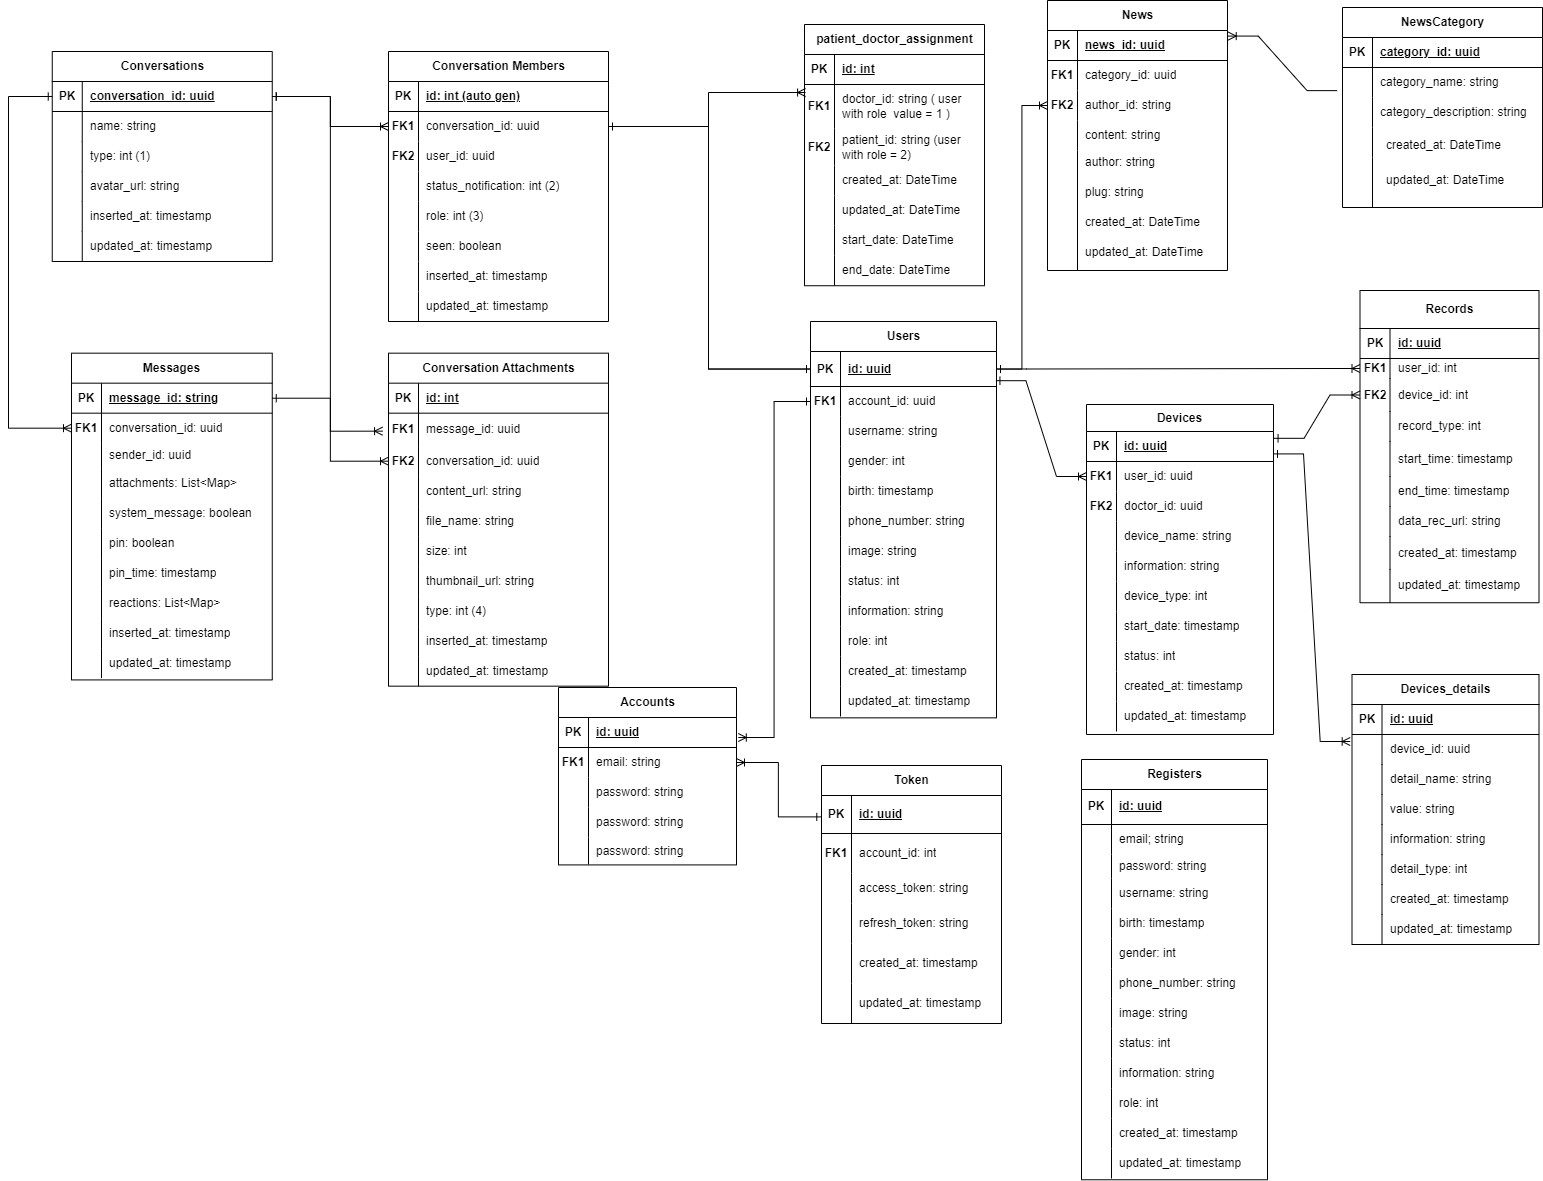
\includegraphics[width=15cm,height=15cm]{Images/system/fmECG_database.png}
	\caption[Sơ đồ ERD]{\bfseries \fontsize{12pt}{0pt}\selectfont Sơ đồ ERD}
	\label{fmECG_architecture-Database}
\end{figure}

\subsection{Thiết kế giao diện}

% Ứng dụng được thiết kế với giao diện hiện đại, sử dụng tông màu chủ đạo là trắng và xanh dương, mang lại cảm giác trang nhã và chuyên nghiệp, đồng thời phù hợp với hình ảnh đặc trưng của lĩnh vực y tế. Sự kết hợp này không chỉ tạo ấn tượng về sự tin cậy mà còn mang đến trải nghiệm người dùng dễ chịu, thân thiện.

% Dưới đây là các giao diện được em thiết kế trong App: 
% \begin{figure}[H]
% 	\centering
% 	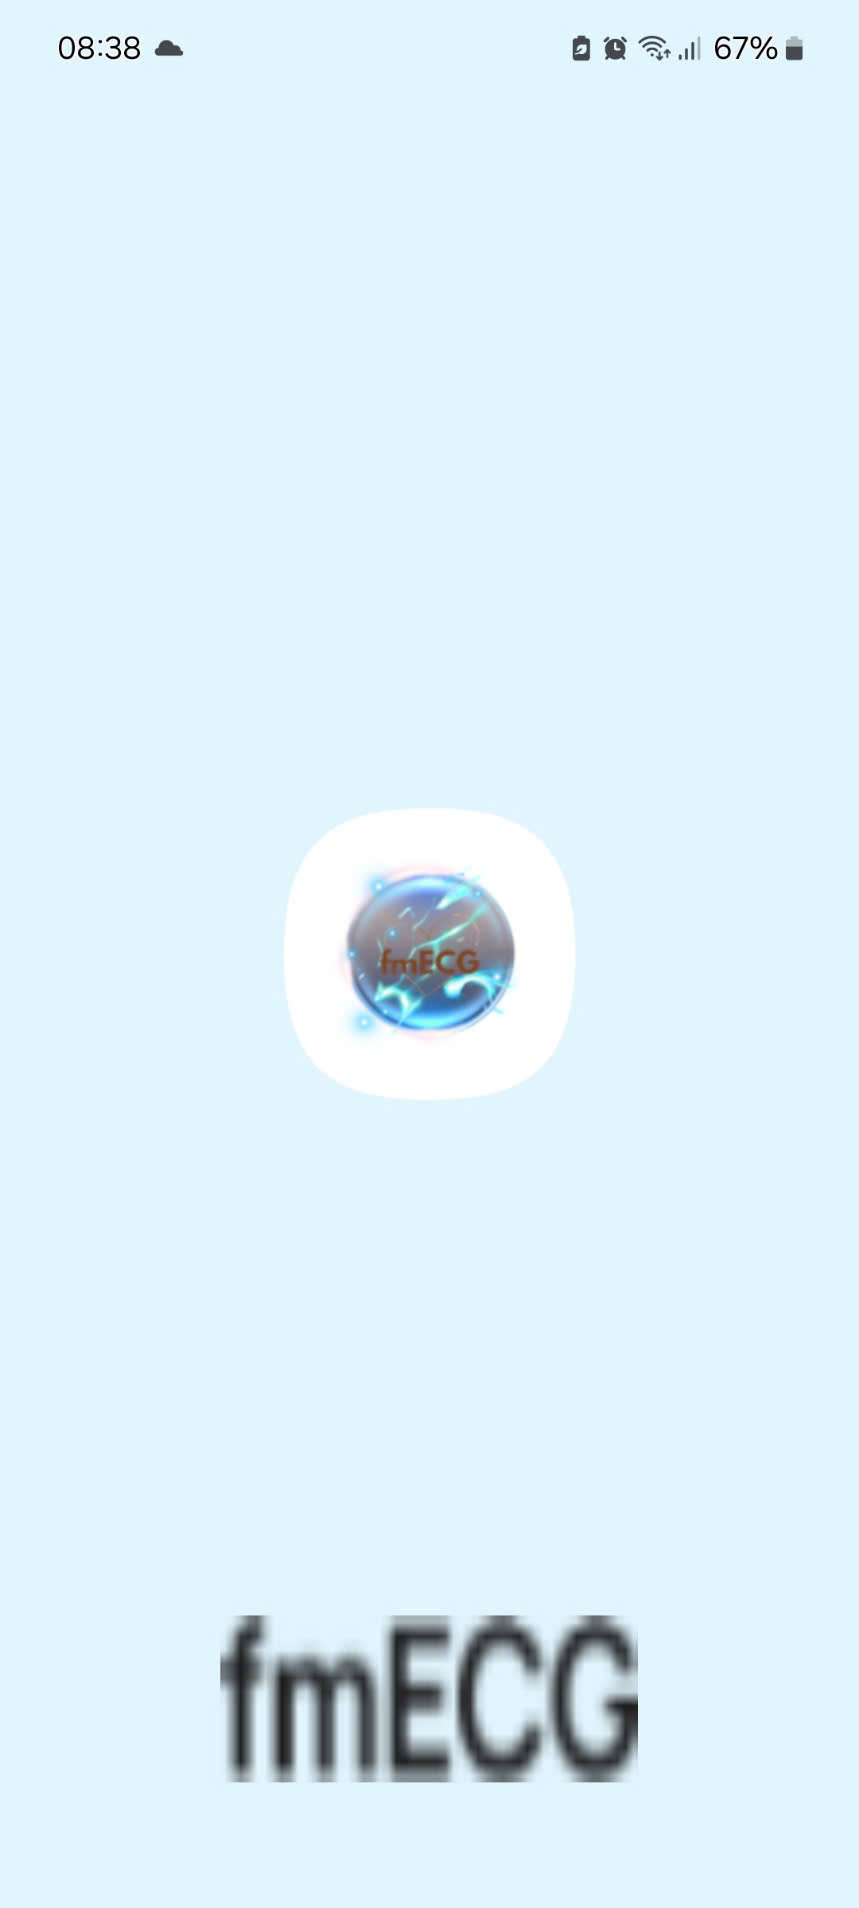
\includegraphics[width=8.5cm,height=18cm]{Images/AppUI/startApp.jpg}
% 	\caption[Giao diện khởi động app]{\bfseries \fontsize{12pt}{0pt}\selectfont Giao diện khởi động app}
% 	\label{startApp}
% \end{figure}
% Hình ảnh hiển thị biểu tượng chính của ứng dụng với nền màu xanh nhạt, mang lại cảm giác nhẹ nhàng và thân thiện với người dùng. Biểu tượng trung tâm là một quả cầu năng lượng với dòng chữ "fmECG," được tô điểm bằng hiệu ứng ánh sáng động, tượng trưng cho sự liên kết giữa công nghệ và y học hiện đại.
% \begin{figure}[H]
% 	\centering
% 	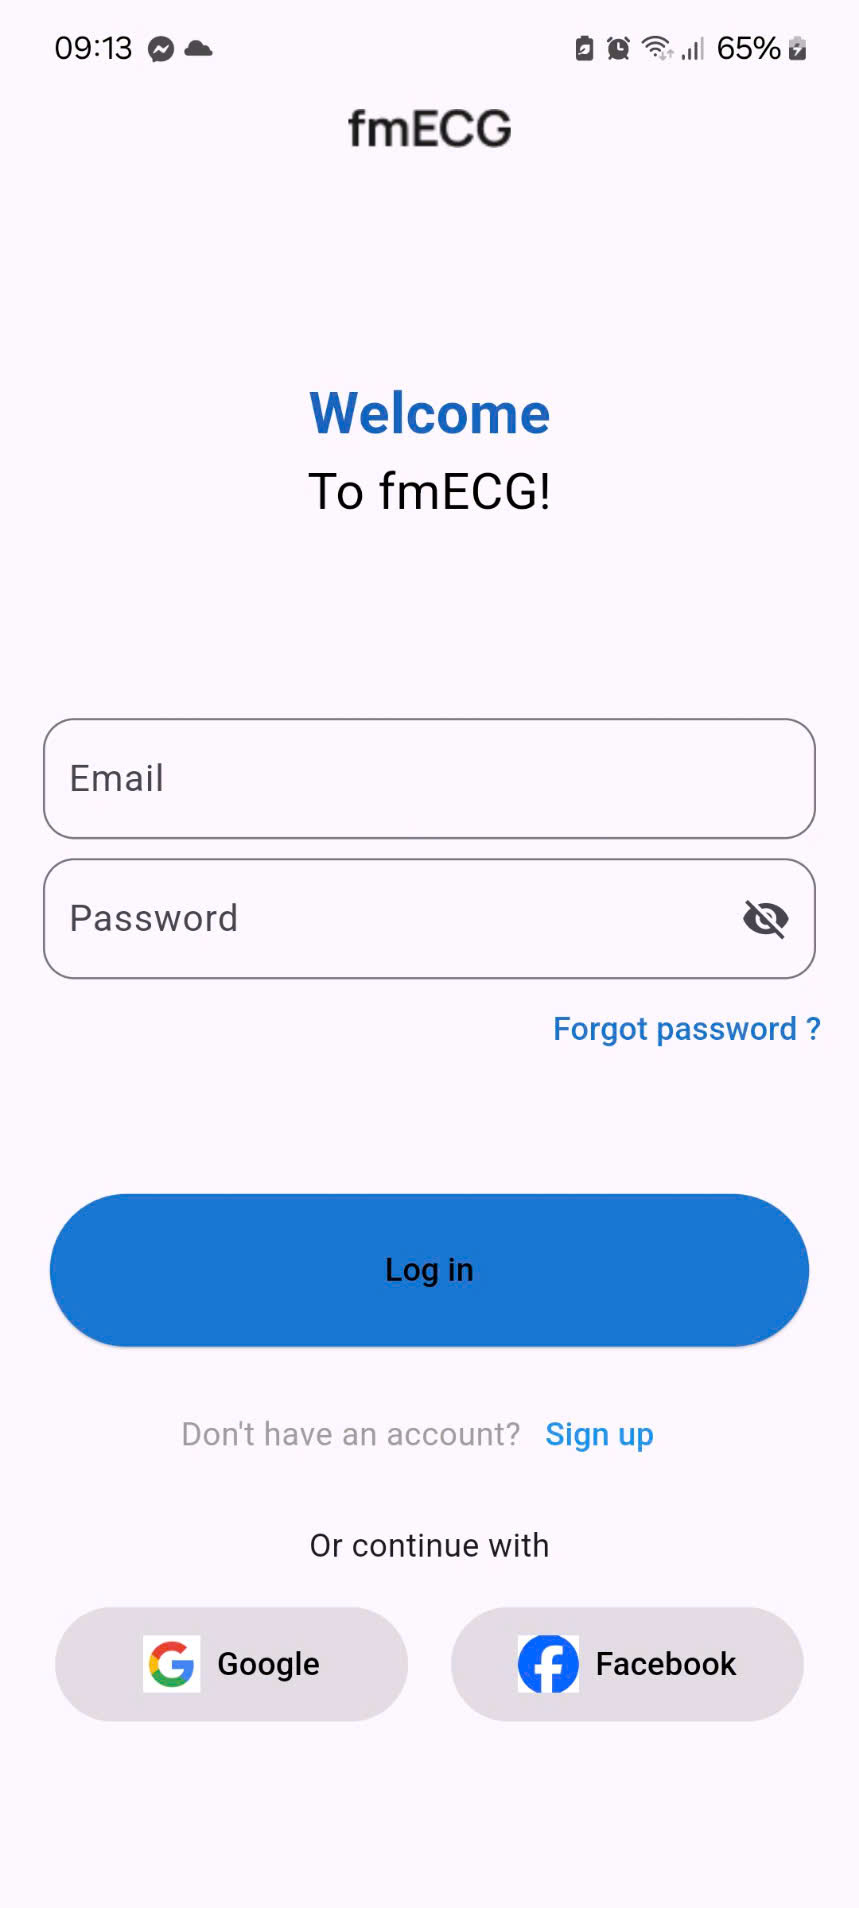
\includegraphics[width=8.5cm,height=18cm]{Images/AppUI/login.jpg}
% 	\caption[Giao diện trang đăng nhập]{\bfseries \fontsize{12pt}{0pt}\selectfont Giao diện trang đăng nhập}
% 	\label{login}
% \end{figure}
% Giao diện đăng nhập của ứng dụng "fmECG" được thiết kế đơn giản và thân thiện với người dùng. Ở phía trên cùng, tên ứng dụng "fmECG" được hiển thị rõ ràng, giúp người dùng dễ dàng nhận diện thương hiệu. Phía dưới là thông điệp chào mừng "Welcome to fmECG!" nhằm tạo cảm giác thân thiện và chuyên nghiệp. Giao diện cung cấp hai ô nhập thông tin: một ô dành cho "Email" và một ô cho "Password," với biểu tượng mắt đi kèm để hỗ trợ người dùng kiểm tra mật khẩu đã nhập.

% \begin{figure}[H] \centering 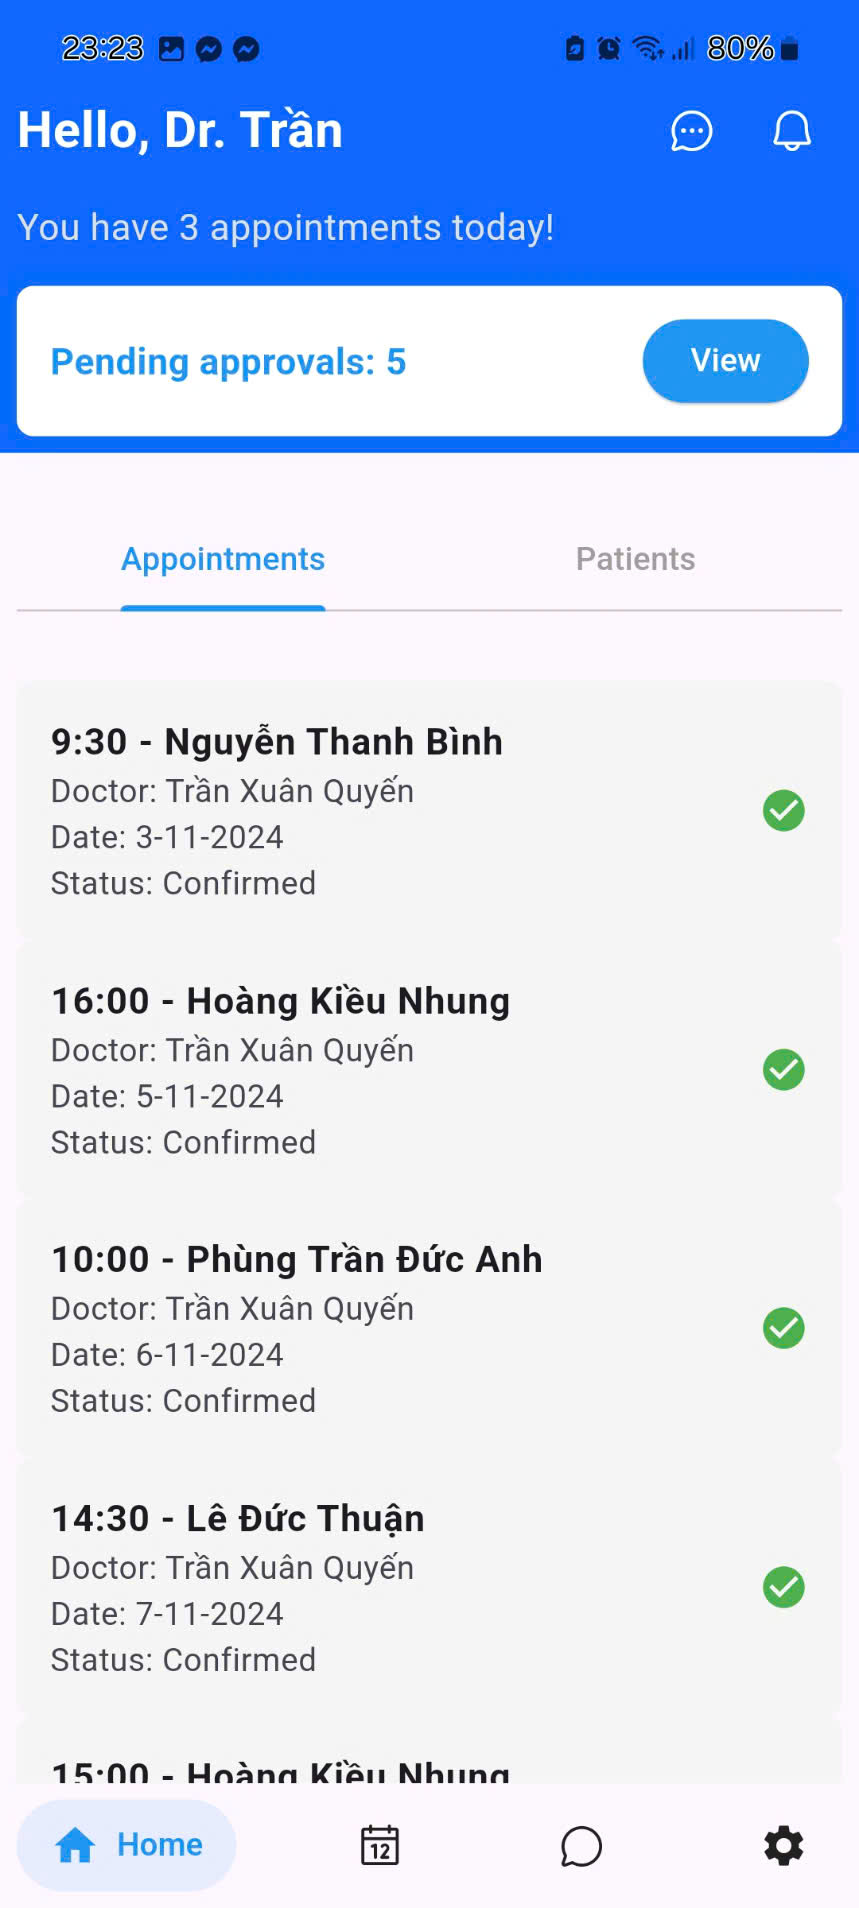
\includegraphics[width=8.5cm,height=18cm]{Images/AppUI/homePage1Doctor.jpg} \caption[Giao diện trang chủ của bác sĩ]{\bfseries \fontsize{12pt}{0pt}\selectfont Giao diện trang chủ của bác sĩ} \label{homeDoctor} \end{figure} 
% Trang chủ của bác sĩ được thiết kế để cung cấp thông tin tổng quan nhanh chóng và rõ ràng. Phần trên cùng hiển thị lời chào cá nhân hóa với số lượng cuộc hẹn trong ngày, đi kèm hai biểu tượng tin nhắn và thông báo ở góc phải để bác sĩ dễ dàng theo dõi thông tin quan trọng. Ngoài ra, mục "Pending approvals" hiển thị số yêu cầu đang chờ xử lý với nút "View" để chuyển hướng đến chi tiết. Phần dưới là danh sách các cuộc hẹn đã xác nhận, bao gồm thông tin thời gian, bệnh nhân, và trạng thái.

% \begin{figure}[H] \centering 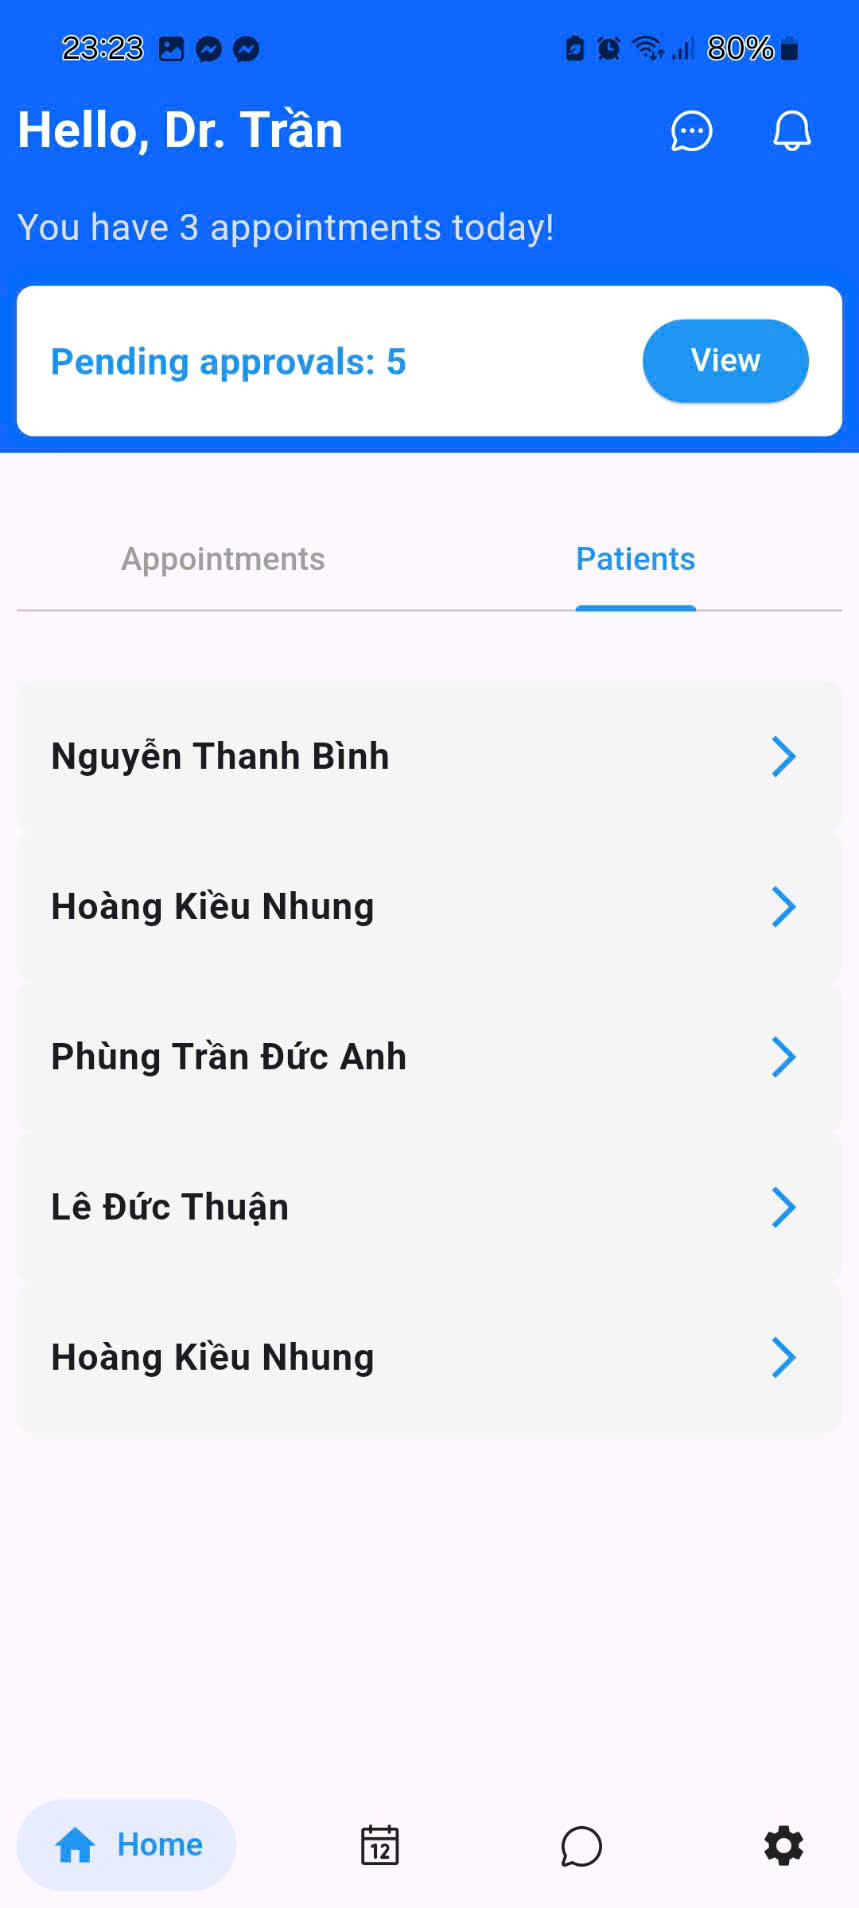
\includegraphics[width=8.5cm,height=18cm]{Images/AppUI/homePage2Doctor.jpg} \caption[Giao diện danh sách bệnh nhân của bác sĩ]{\bfseries \fontsize{12pt}{0pt}\selectfont Giao diện danh sách bệnh nhân của bác sĩ} \label{patientListDoctor} \end{figure} 
% Tab "Patients" trong giao diện bác sĩ hiển thị danh sách các bệnh nhân dưới dạng các mục riêng biệt. Mỗi mục bao gồm tên bệnh nhân cùng nút điều hướng để truy cập nhanh vào hồ sơ chi tiết của từng người. Thiết kế này giúp bác sĩ dễ dàng quản lý và theo dõi thông tin bệnh nhân của mình.

% \begin{figure}[H] \centering 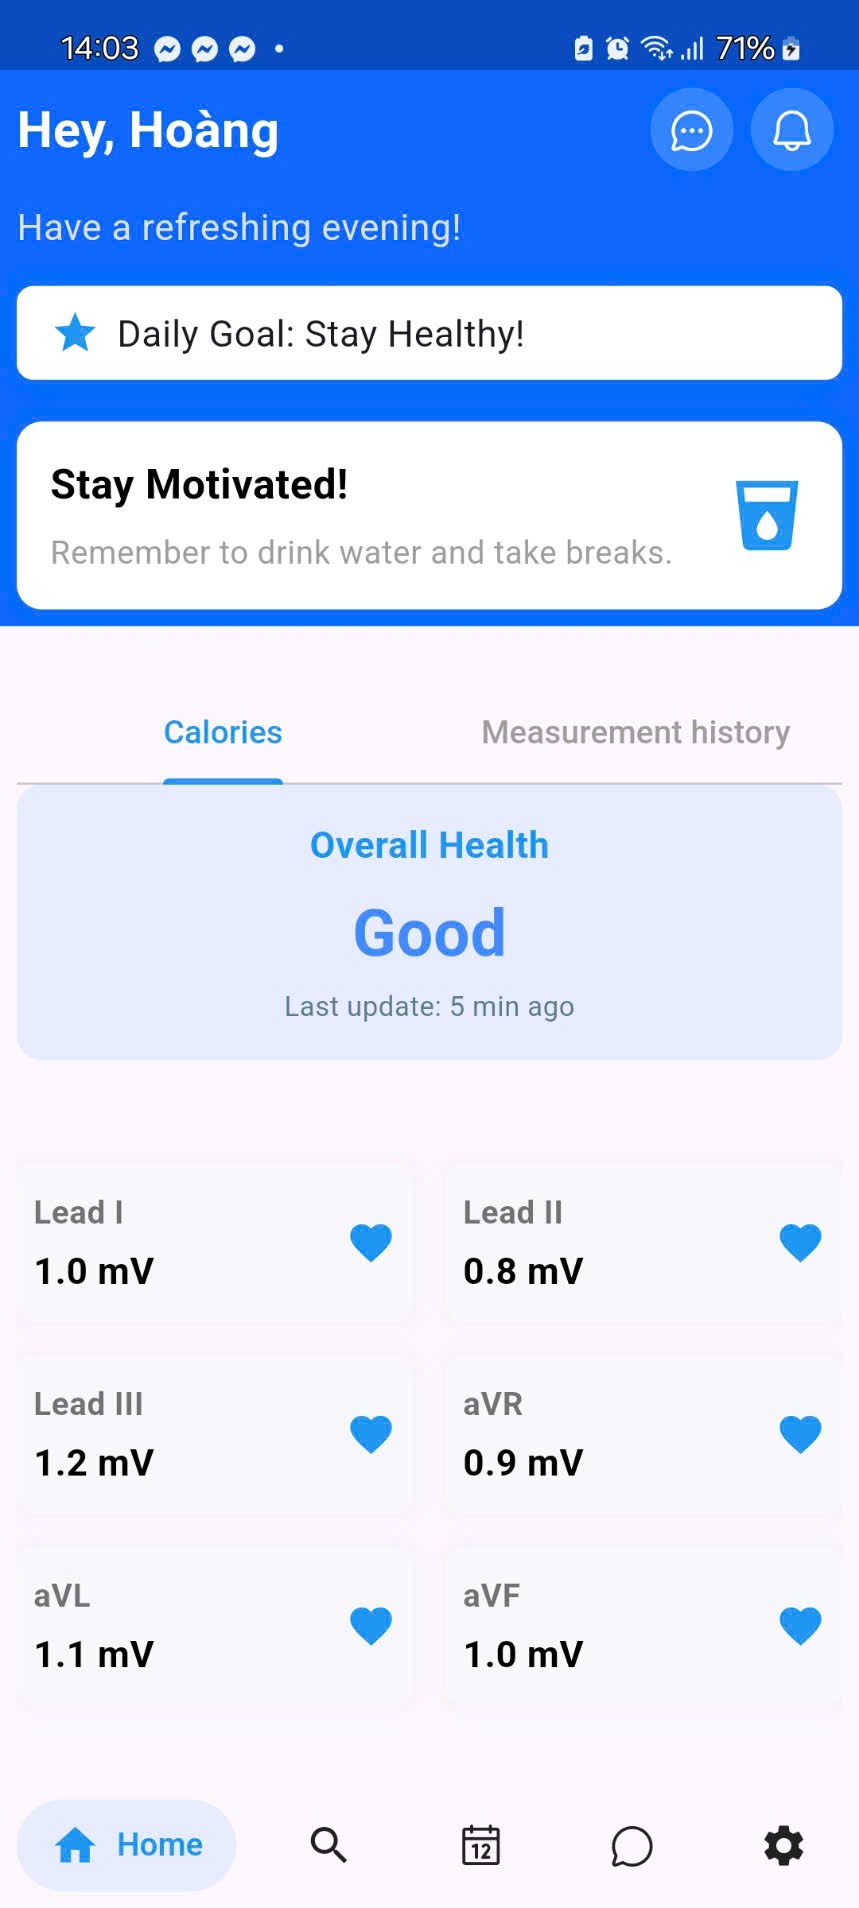
\includegraphics[width=8.5cm,height=18cm]{Images/AppUI/homePagePatient.jpg} \caption[Giao diện thông tin sức khỏe của bệnh nhân]{\bfseries \fontsize{12pt}{0pt}\selectfont Giao diện thông tin sức khỏe của bệnh nhân} \label{healthInfoPatient} \end{figure}
% Giao diện của bệnh nhân tập trung vào việc hiển thị trạng thái sức khỏe tổng quan với đánh giá "Overall Health: Good" được cập nhật gần nhất. Bên dưới là 6 số liệu liên quan đến điện tim, được trình bày rõ ràng và dễ hiểu. Những số liệu này đại diện cho các thông tin đo lường quan trọng, giúp bệnh nhân theo dõi tình trạng sức khỏe tim mạch của mình một cách trực quan. Giao diện hiện đại và thân thiện, mang đến trải nghiệm sử dụng thuận tiện và tối ưu.

% Sang giao diện đặt lịch:
% \begin{figure}[H]
% 	\centering
% 	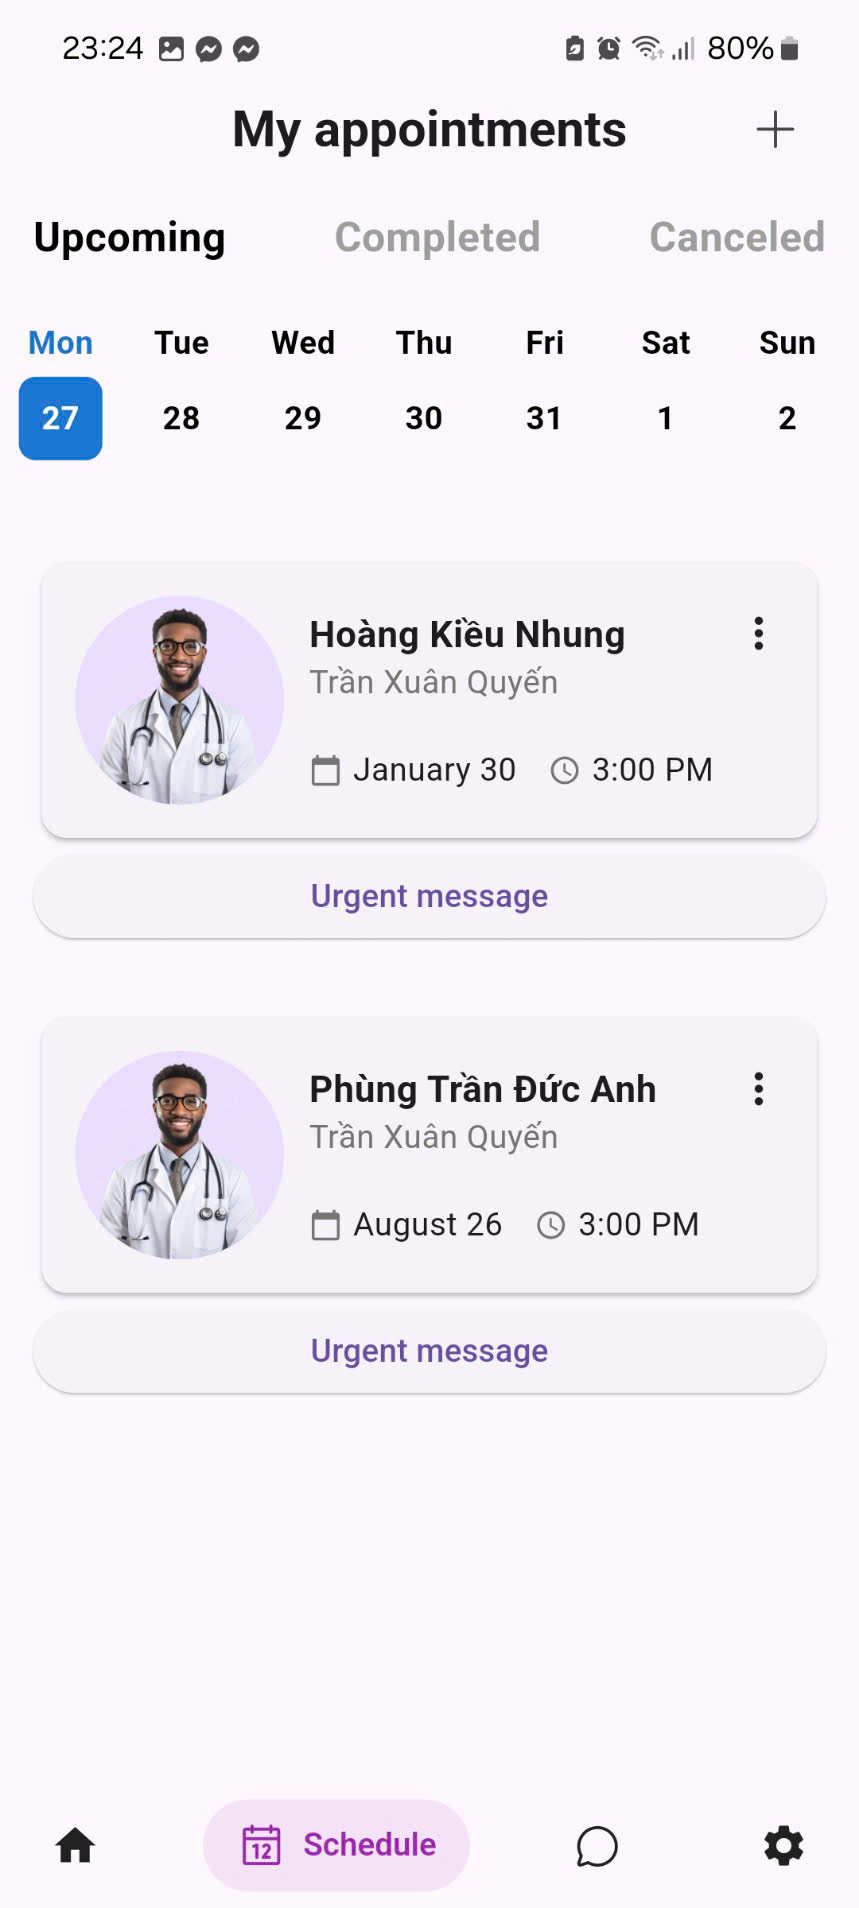
\includegraphics[width=8.5cm,height=18cm]{Images/AppUI/scheduleUpComing.jpg}
% 	\caption[Giao diện quản lý lịch của bác sĩ]{\bfseries \fontsize{12pt}{0pt}\selectfont Giao diện quản lý lịch của bác sĩ}
% 	\label{scheduleDoctor}
% \end{figure}
% Giao diện quản lý lịch của bác sĩ được chia thành ba tab chính: \textbf{Upcoming}, \textbf{Completed}, và \textbf{Canceled}. Tab \textbf{Upcoming} hiển thị danh sách các cuộc hẹn sắp tới với thông tin chi tiết như tên bệnh nhân, ngày và giờ hẹn, cùng nút "Urgent message" để liên lạc khẩn cấp khi cần thiết. 


% \begin{figure}[H]
% 	\centering
% 	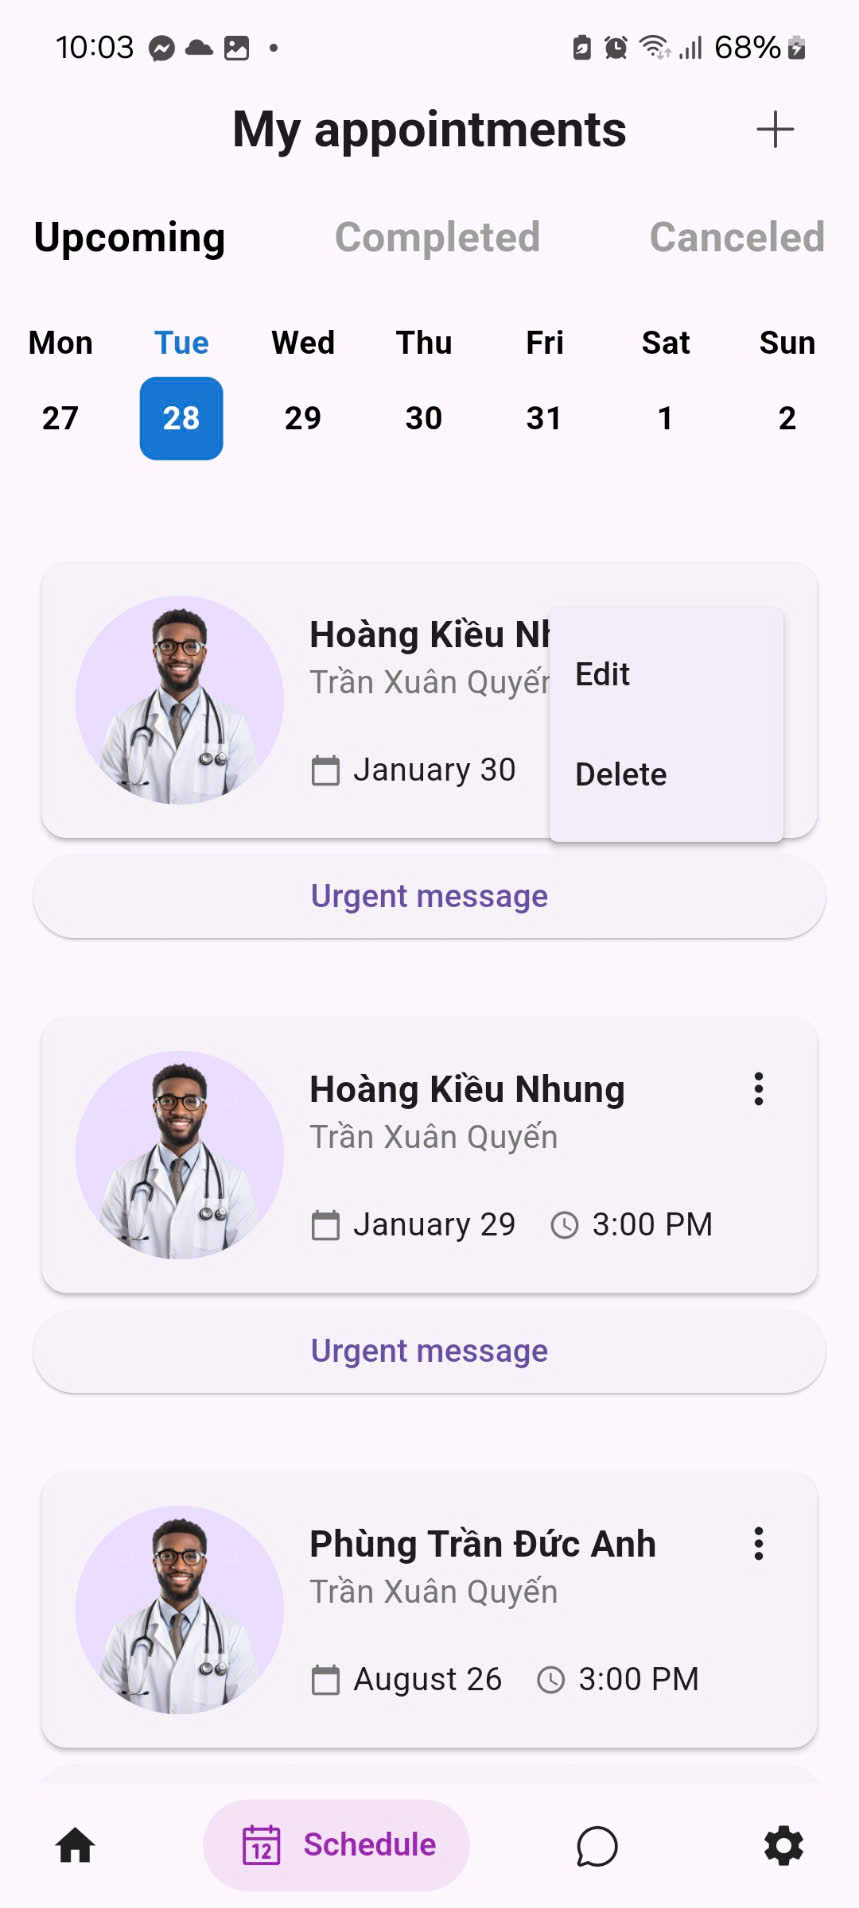
\includegraphics[width=8.5cm,height=18cm]{Images/AppUI/optionSchedule.jpg}
% 	\caption[Tùy chọn hủy lịch hẹn trong tab Upcoming]{\bfseries \fontsize{12pt}{0pt}\selectfont Tùy chọn hủy lịch hẹn trong tab Upcoming}
% 	\label{upcomingOptions}
% \end{figure}
% Trong tab \textbf{Upcoming}, mỗi cuộc hẹn đều có biểu tượng dấu ba chấm ở góc phải, cho phép bác sĩ truy cập vào các tùy chọn bổ sung. Một trong số đó là chức năng \textbf{Hủy lịch hẹn}. Khi nhấn vào tùy chọn này, một cửa sổ mới sẽ xuất hiện, yêu cầu bác sĩ nhập lý do hủy lịch.

% \begin{figure}[H]
% 	\centering
% 	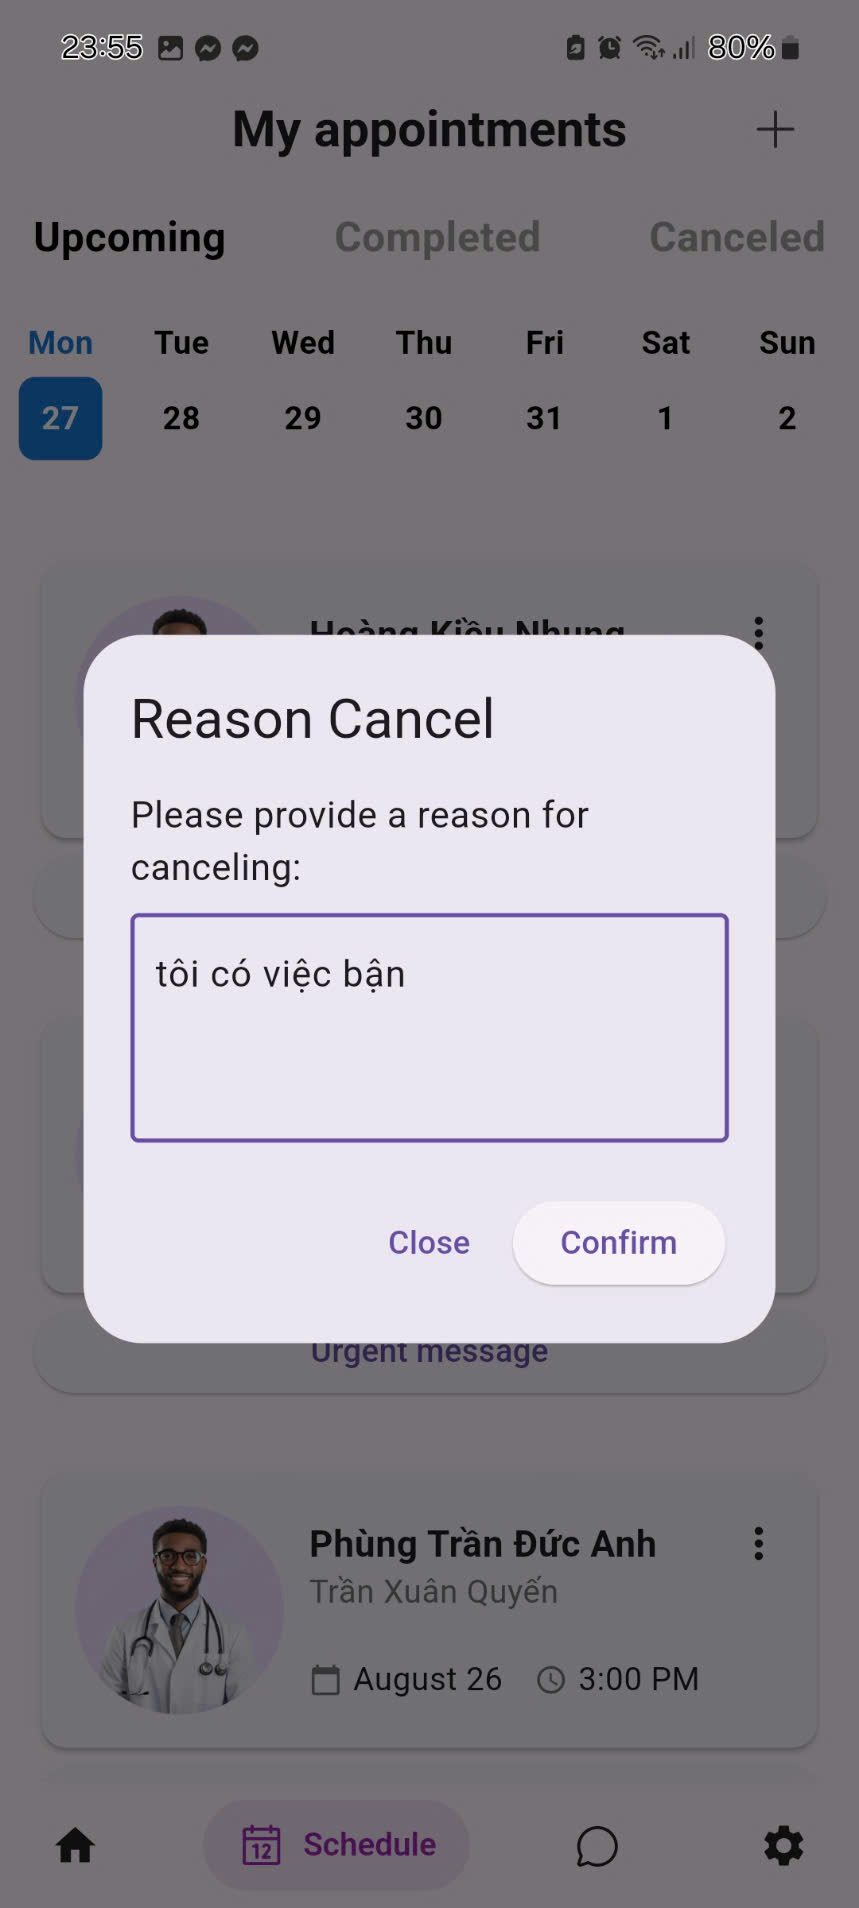
\includegraphics[width=8.5cm,height=18cm]{Images/AppUI/cancelledSchedule.jpg}
% 	\caption[Giao diện nhập lý do hủy lịch hẹn]{\bfseries \fontsize{12pt}{0pt}\selectfont Giao diện nhập lý do hủy lịch hẹn}
% 	\label{cancelAppointment}
% \end{figure}
% Giao diện nhập lý do hủy lịch hẹn cung cấp một ô nhập liệu để bác sĩ điền thông tin giải thích lý do hủy cuộc hẹn. Phía dưới là hai nút chức năng:
% \begin{itemize}
% 	\item \textbf{Cancel Appointment}: Xác nhận hủy lịch hẹn sau khi lý do được nhập.
% 	\item \textbf{Close}: Đóng cửa sổ mà không thực hiện thay đổi.
% \end{itemize}
% Chức năng này đảm bảo bác sĩ có thể quản lý lịch hẹn linh hoạt, đồng thời cung cấp thông tin rõ ràng cho bệnh nhân về lý do hủy lịch.


% Tab \textbf{Completed} tập hợp các cuộc hẹn đã hoàn thành. Khi nhấn vào một mục trong danh sách, bác sĩ sẽ được chuyển đến cửa sổ chi tiết, hiển thị thông tin bệnh nhân như tên, tuổi, giới tính, và số điện thoại, cùng với các tùy chọn thao tác như nhập thông tin chẩn đoán và tạo lịch tái khám. Tab \textbf{Canceled} cho phép bác sĩ theo dõi các cuộc hẹn đã bị hủy, hỗ trợ việc quản lý lịch sử làm việc dễ dàng hơn.

% \begin{figure}[H]
% 	\centering
% 	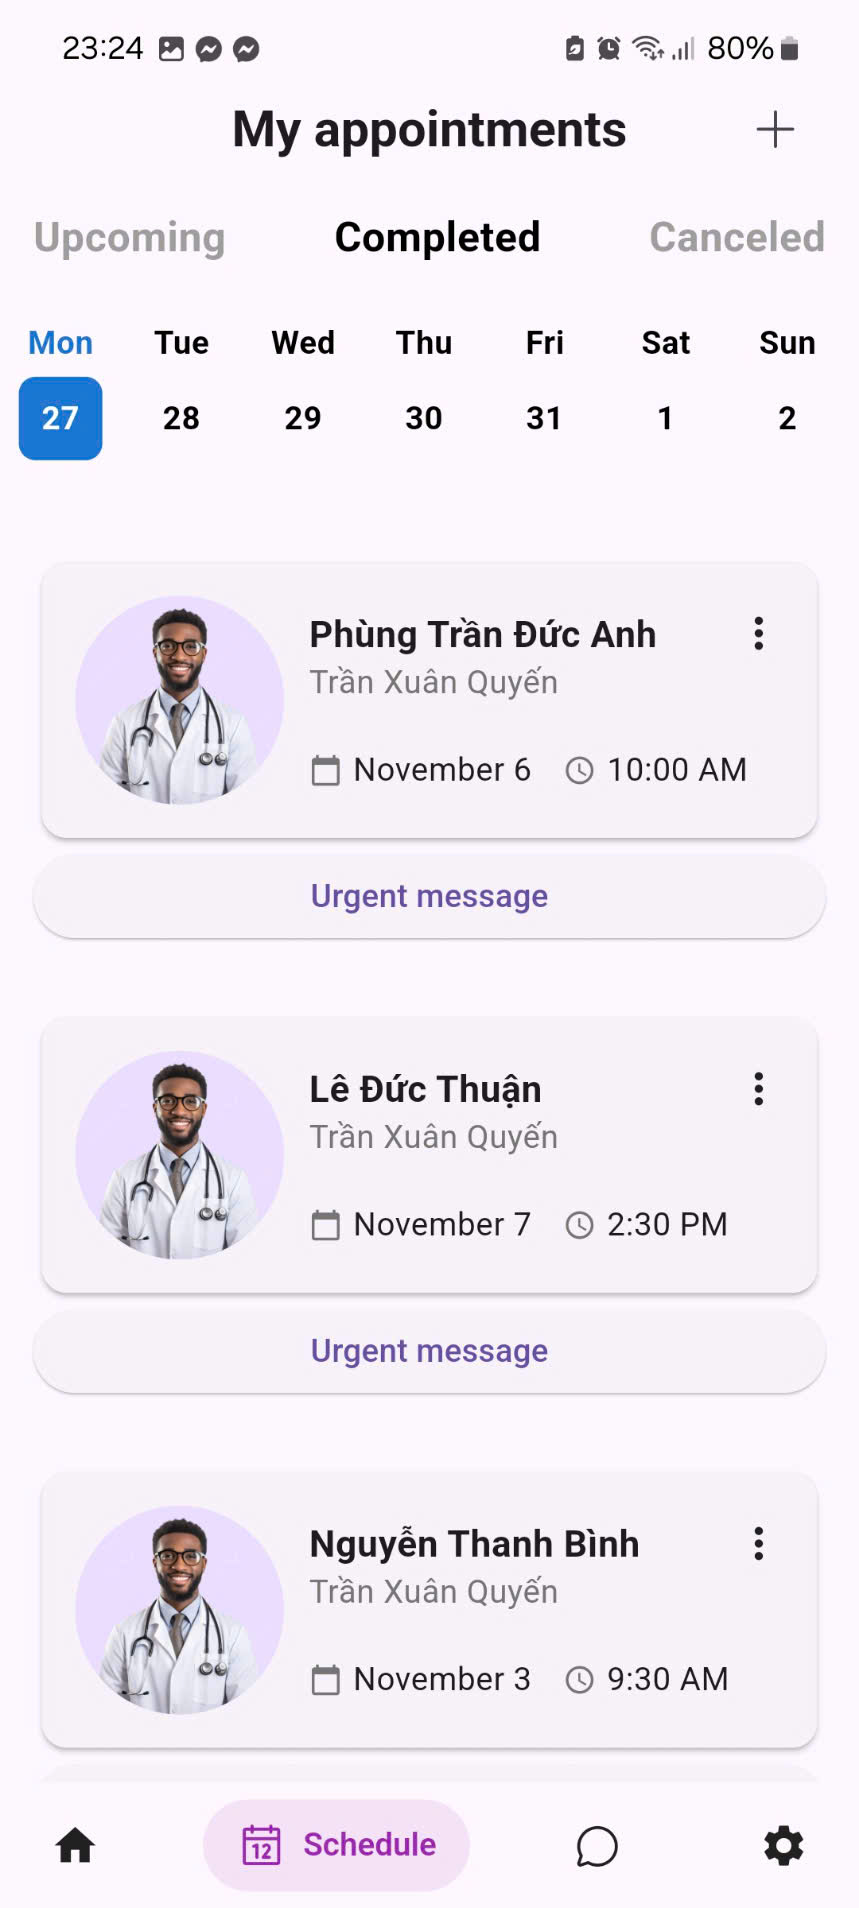
\includegraphics[width=8.5cm,height=18cm]{Images/AppUI/scheduleCompleted.jpg}
% 	\caption[Chi tiết thông tin bệnh nhân từ lịch đã hoàn thành]{\bfseries \fontsize{12pt}{0pt}\selectfont Chi tiết thông tin bệnh nhân từ lịch đã hoàn thành}
% 	\label{patientInfo}
% \end{figure}
% Khi truy cập vào thông tin chi tiết từ tab \textbf{Completed}, bác sĩ sẽ thấy toàn bộ thông tin về bệnh nhân, bao gồm tên, tuổi, giới tính, và số điện thoại. Bên dưới là các nút chức năng như:
% \begin{itemize}
% 	\item \textbf{Chẩn đoán}: Cho phép bác sĩ nhập hoặc chỉnh sửa thông tin chẩn đoán cho bệnh nhân.
% 	\item \textbf{Tạo lịch tái khám}: Hỗ trợ bác sĩ đặt lịch tái khám mới với giao diện chọn ngày và giờ trực quan.
% 	\item \textbf{Đóng cửa sổ}: Kết thúc thao tác và quay lại danh sách.
% \end{itemize}

% \begin{figure}[H]
% 	\centering
% 	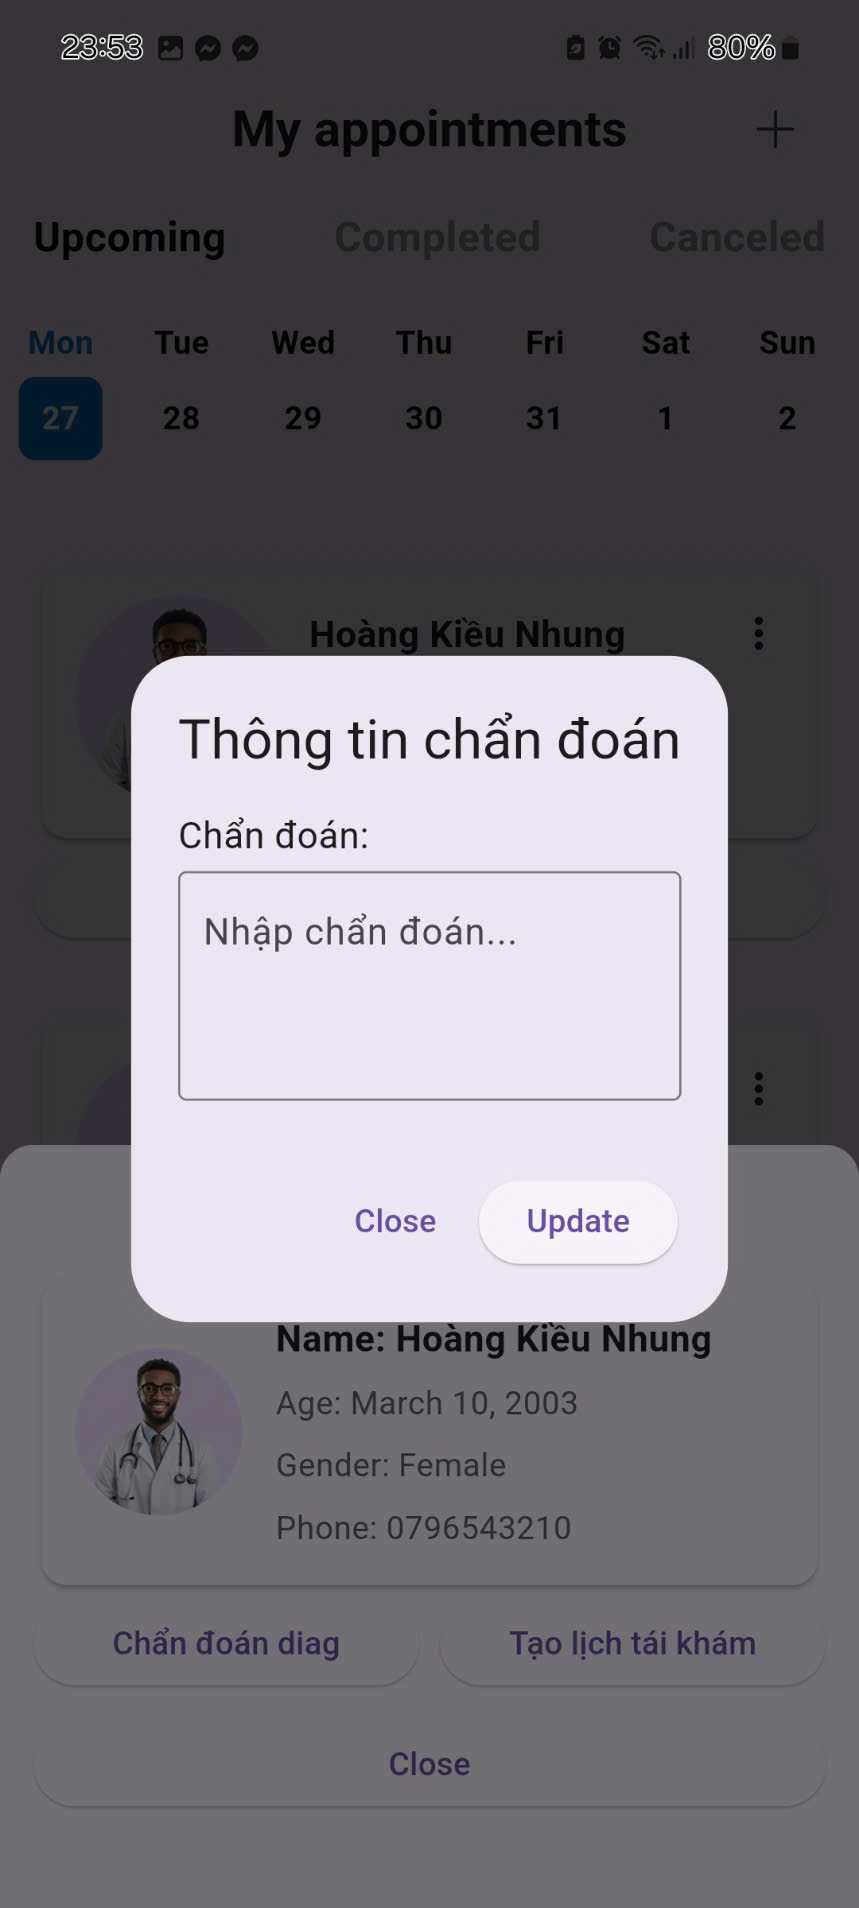
\includegraphics[width=8.5cm,height=18cm]{Images/AppUI/blockInputDIag.jpg}
% 	\caption[Cửa sổ cập nhật thông tin chẩn đoán]{\bfseries \fontsize{12pt}{0pt}\selectfont Cửa sổ cập nhật thông tin chẩn đoán}
% 	\label{diagnosisUpdate}
% \end{figure}
% Giao diện cập nhật chẩn đoán cung cấp một ô nhập liệu để bác sĩ thêm hoặc chỉnh sửa nội dung chẩn đoán, đi kèm nút \textbf{Update} để lưu thông tin mới.

% \begin{figure}[H]
% 	\centering
% 	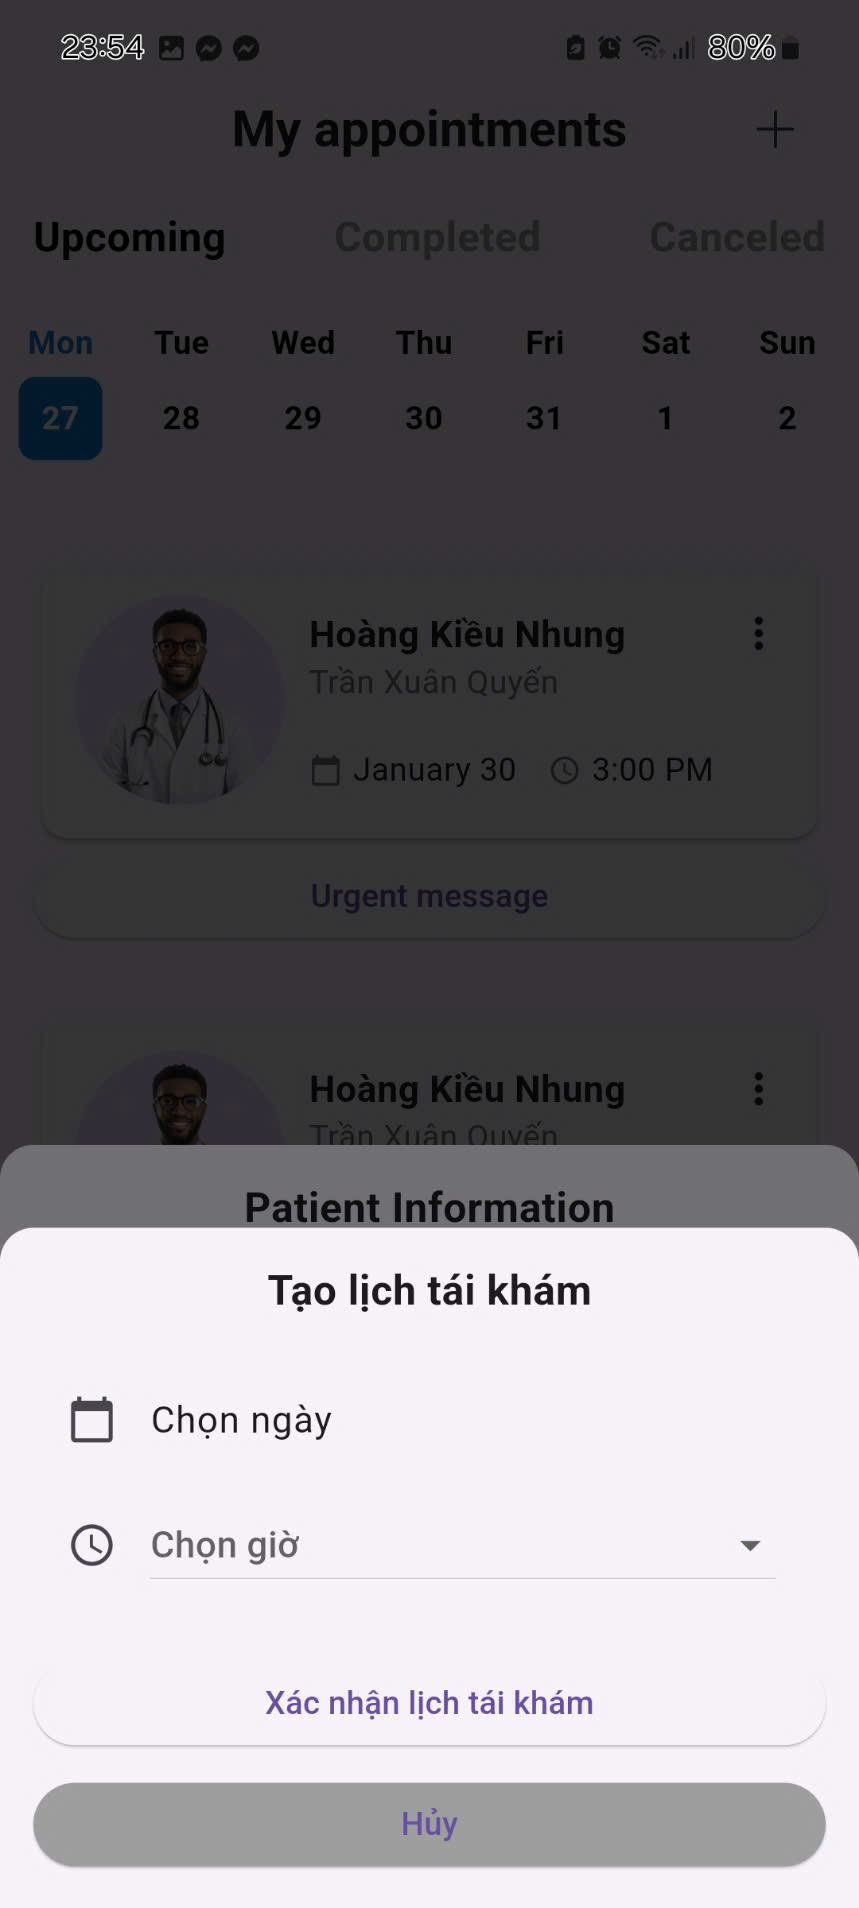
\includegraphics[width=8.5cm,height=18cm]{Images/AppUI/repickSchedule2.jpg}
% 	\caption[Cửa sổ tạo lịch tái khám]{\bfseries \fontsize{12pt}{0pt}\selectfont Cửa sổ tạo lịch tái khám}
% 	\label{reschedule}
% \end{figure}
% Giao diện đặt lịch tái khám cho phép bác sĩ chọn ngày và giờ, sau đó xác nhận bằng nút \textbf{Xác nhận lịch tái khám}. Điều này giúp đảm bảo việc quản lý các cuộc hẹn diễn ra mượt mà và hiệu quả.

\subsubsection{Màn hình khởi động và đăng nhập}

\begin{figure}[H]
	\centering
	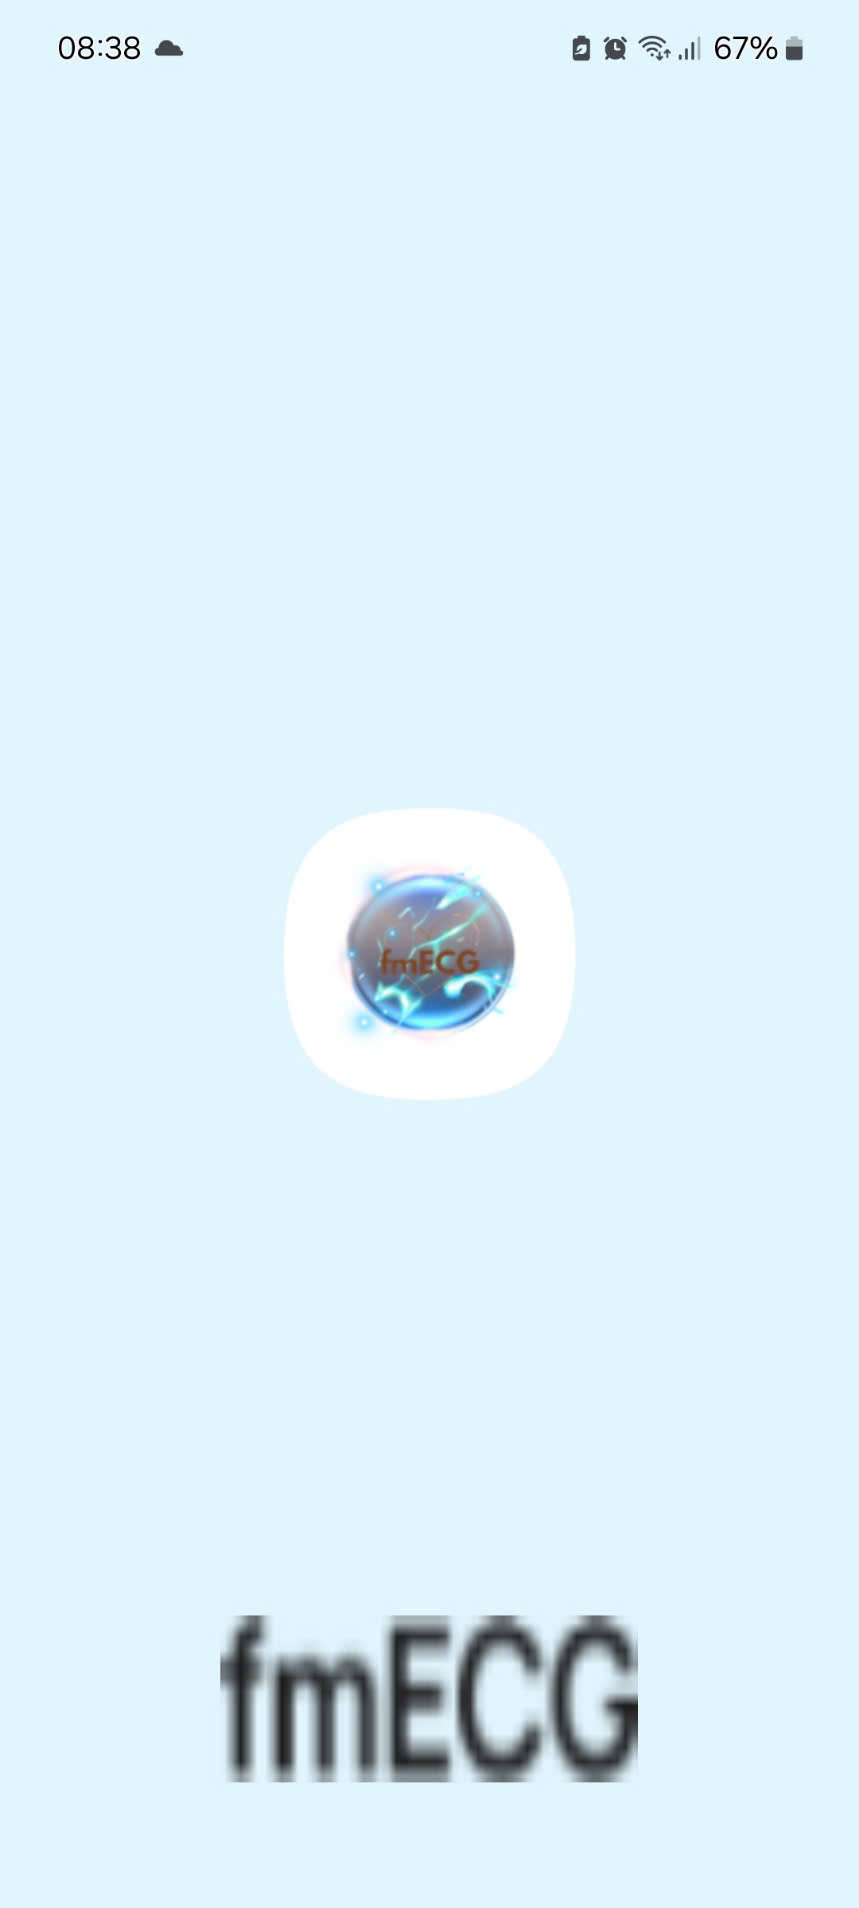
\includegraphics[width=8.5cm,height=18cm]{Images/AppUI/startApp.jpg}
	\caption[Giao diện khởi động app]{\bfseries \fontsize{12pt}{0pt}\selectfont Giao diện khởi động app}
	\label{startApp}
\end{figure}
Hình ảnh hiển thị biểu tượng chính của ứng dụng với nền màu xanh nhạt, mang lại cảm giác nhẹ nhàng và thân thiện với người dùng. Biểu tượng trung tâm là một quả cầu năng lượng với dòng chữ "fmECG," được tô điểm bằng hiệu ứng ánh sáng động, tượng trưng cho sự liên kết giữa công nghệ và y học hiện đại.

\begin{figure}[H]
	\centering
	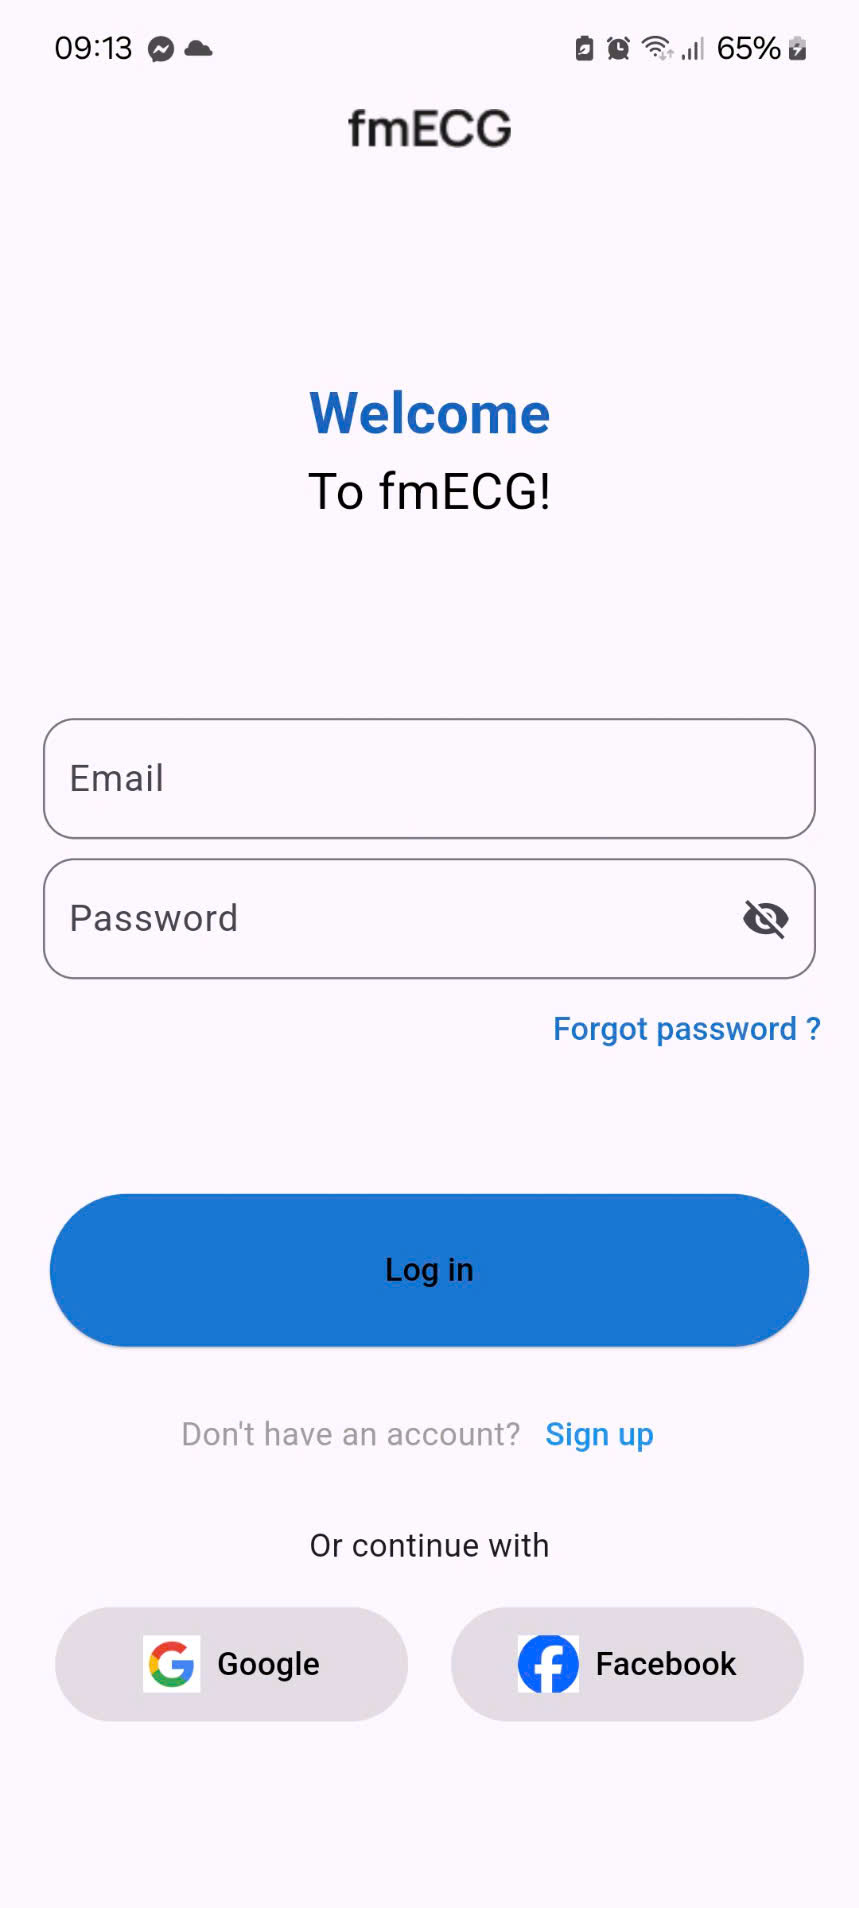
\includegraphics[width=8.5cm,height=18cm]{Images/AppUI/login.jpg}
	\caption[Giao diện trang đăng nhập]{\bfseries \fontsize{12pt}{0pt}\selectfont Giao diện trang đăng nhập}
	\label{login}
\end{figure}
Giao diện đăng nhập của ứng dụng "fmECG" được thiết kế đơn giản và thân thiện với người dùng. Ở phía trên cùng, tên ứng dụng "fmECG" được hiển thị rõ ràng, giúp người dùng dễ dàng nhận diện thương hiệu. Phía dưới là thông điệp chào mừng "Welcome to fmECG!" nhằm tạo cảm giác thân thiện và chuyên nghiệp. Giao diện cung cấp hai ô nhập thông tin: một ô dành cho "Email" và một ô cho "Password," với biểu tượng mắt đi kèm để hỗ trợ người dùng kiểm tra mật khẩu đã nhập.

\subsubsection{Giao diện của bác sĩ (Doctor)}

\begin{figure}[H]
	\centering
	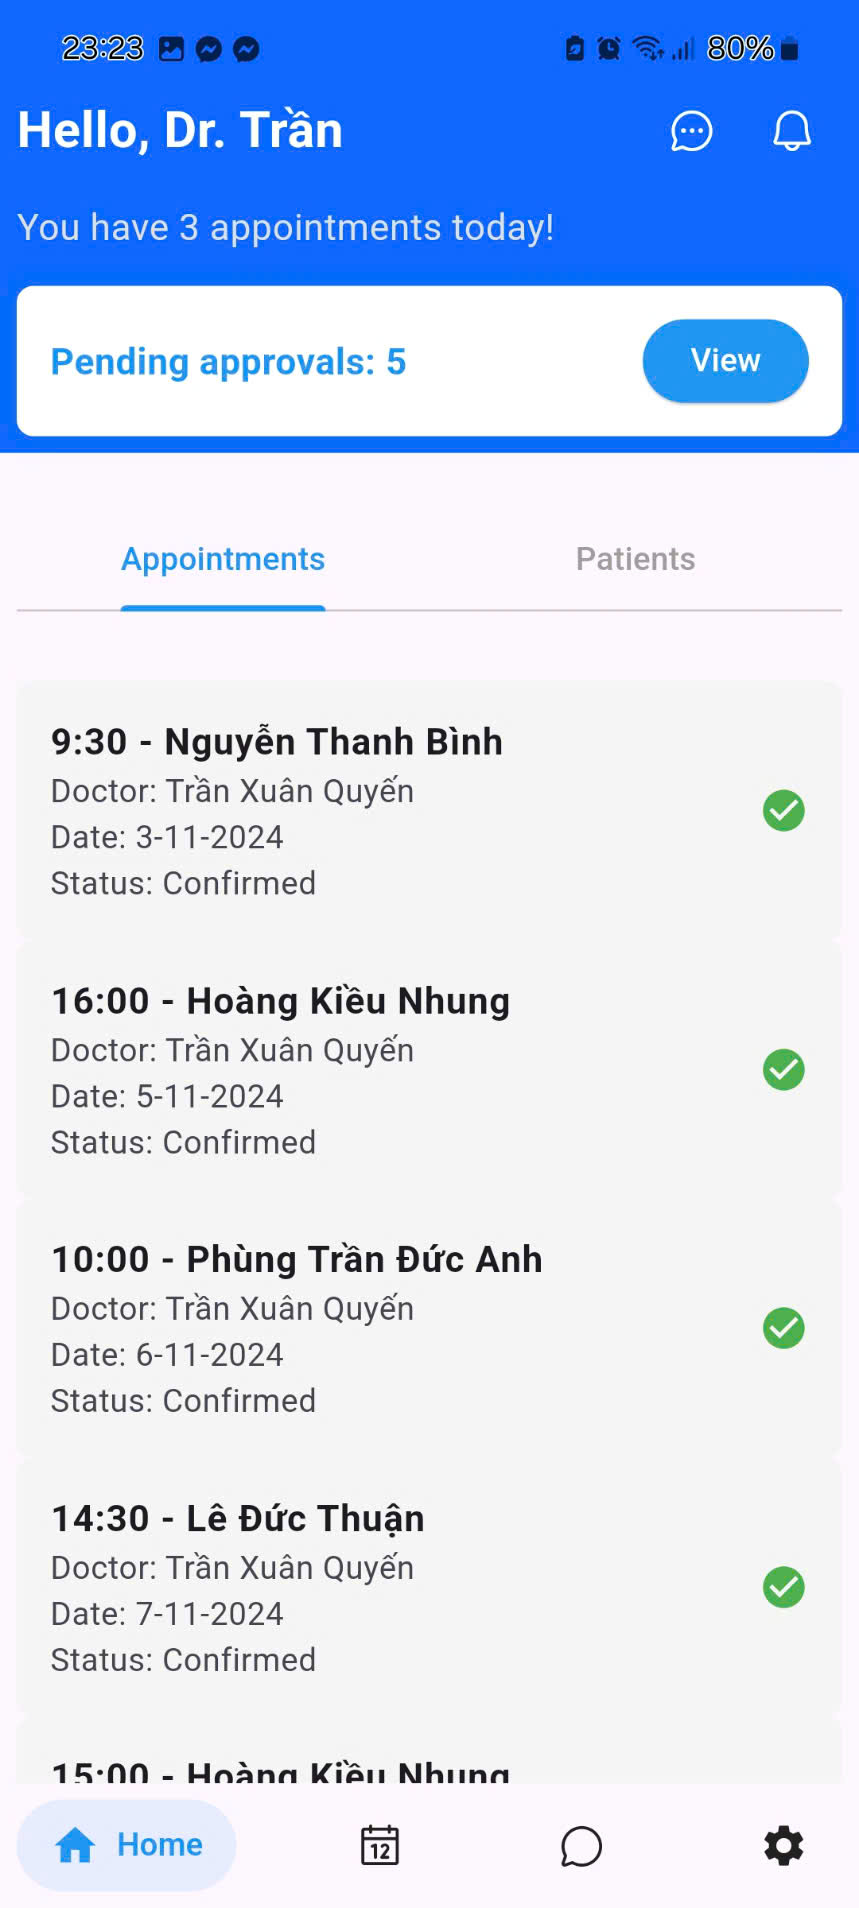
\includegraphics[width=8.5cm,height=18cm]{Images/AppUI/homePage1Doctor.jpg}
	\caption[Giao diện trang chủ của bác sĩ]{\bfseries \fontsize{12pt}{0pt}\selectfont Giao diện trang chủ của bác sĩ}
	\label{homeDoctor}
\end{figure}
Trang chủ của bác sĩ được thiết kế để cung cấp thông tin tổng quan nhanh chóng và rõ ràng. Phần trên cùng hiển thị lời chào cá nhân hóa với số lượng cuộc hẹn trong ngày, đi kèm hai biểu tượng tin nhắn và thông báo ở góc phải để bác sĩ dễ dàng theo dõi thông tin quan trọng. Ngoài ra, mục "Pending approvals" hiển thị số yêu cầu đang chờ xử lý với nút "View" để chuyển hướng đến chi tiết. Phần dưới là danh sách các cuộc hẹn đã xác nhận, bao gồm thông tin thời gian, bệnh nhân, và trạng thái.

\begin{figure}[H]
	\centering
	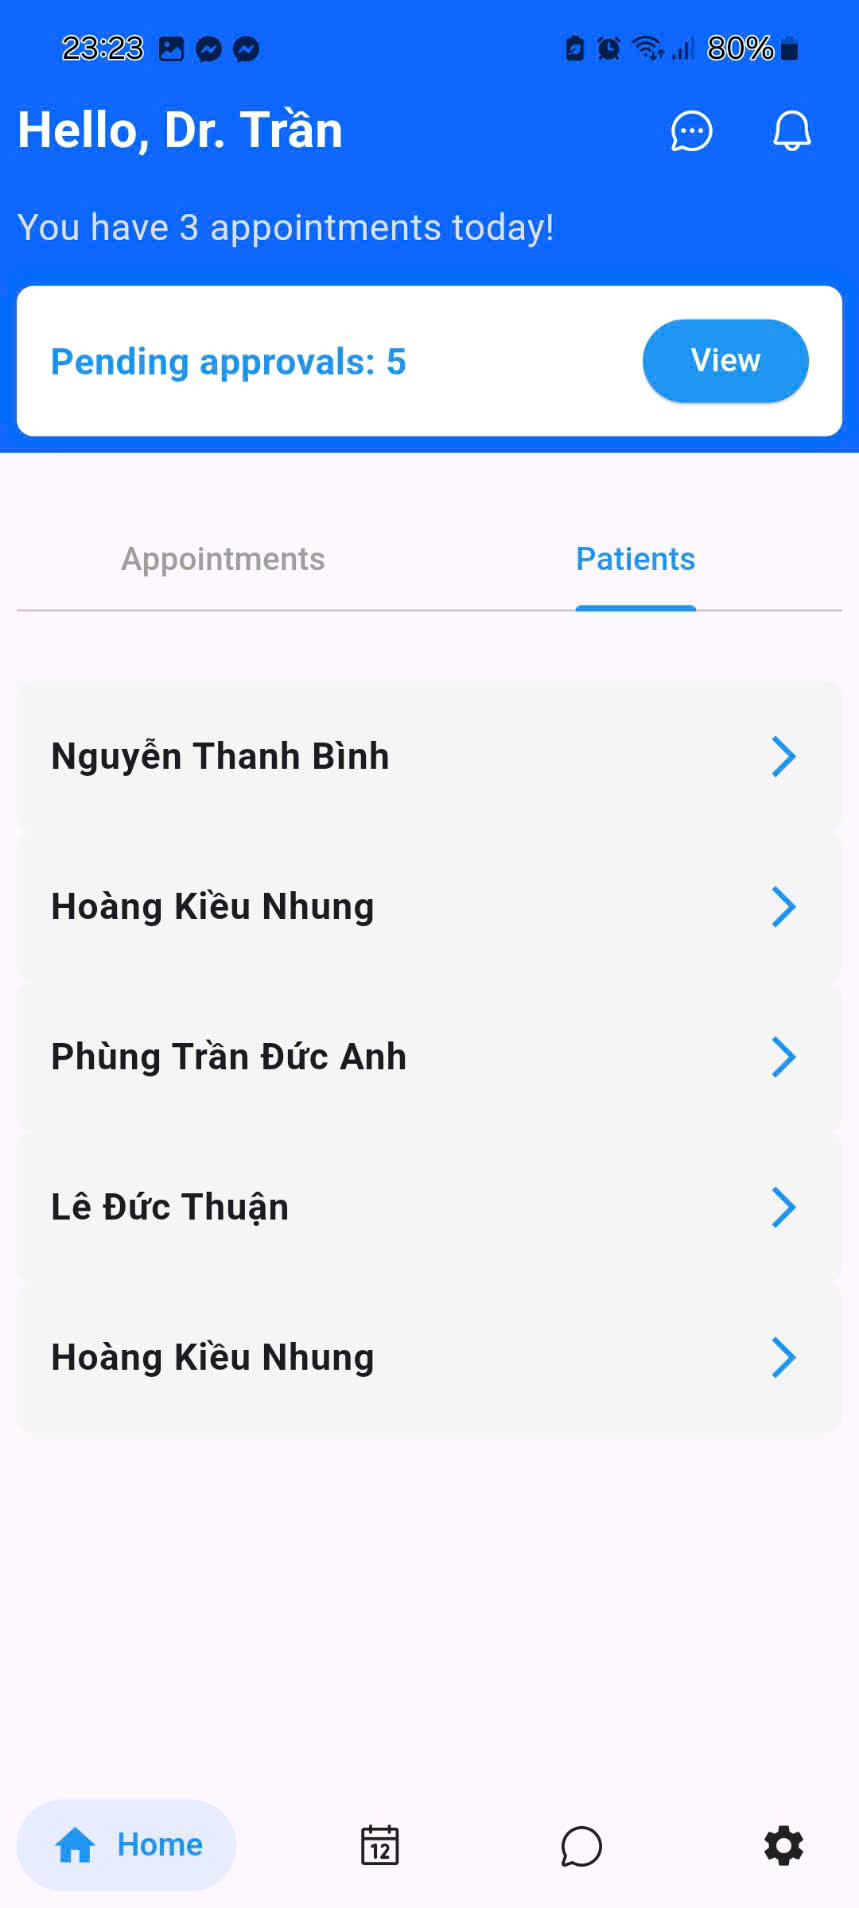
\includegraphics[width=8.5cm,height=18cm]{Images/AppUI/homePage2Doctor.jpg}
	\caption[Giao diện danh sách bệnh nhân của bác sĩ]{\bfseries \fontsize{12pt}{0pt}\selectfont Giao diện danh sách bệnh nhân của bác sĩ}
	\label{patientListDoctor}
\end{figure}
Tab "Patients" trong giao diện bác sĩ hiển thị danh sách các bệnh nhân dưới dạng các mục riêng biệt. Mỗi mục bao gồm tên bệnh nhân cùng nút điều hướng để truy cập nhanh vào hồ sơ chi tiết của từng người.

\begin{figure}[H]
	\centering
	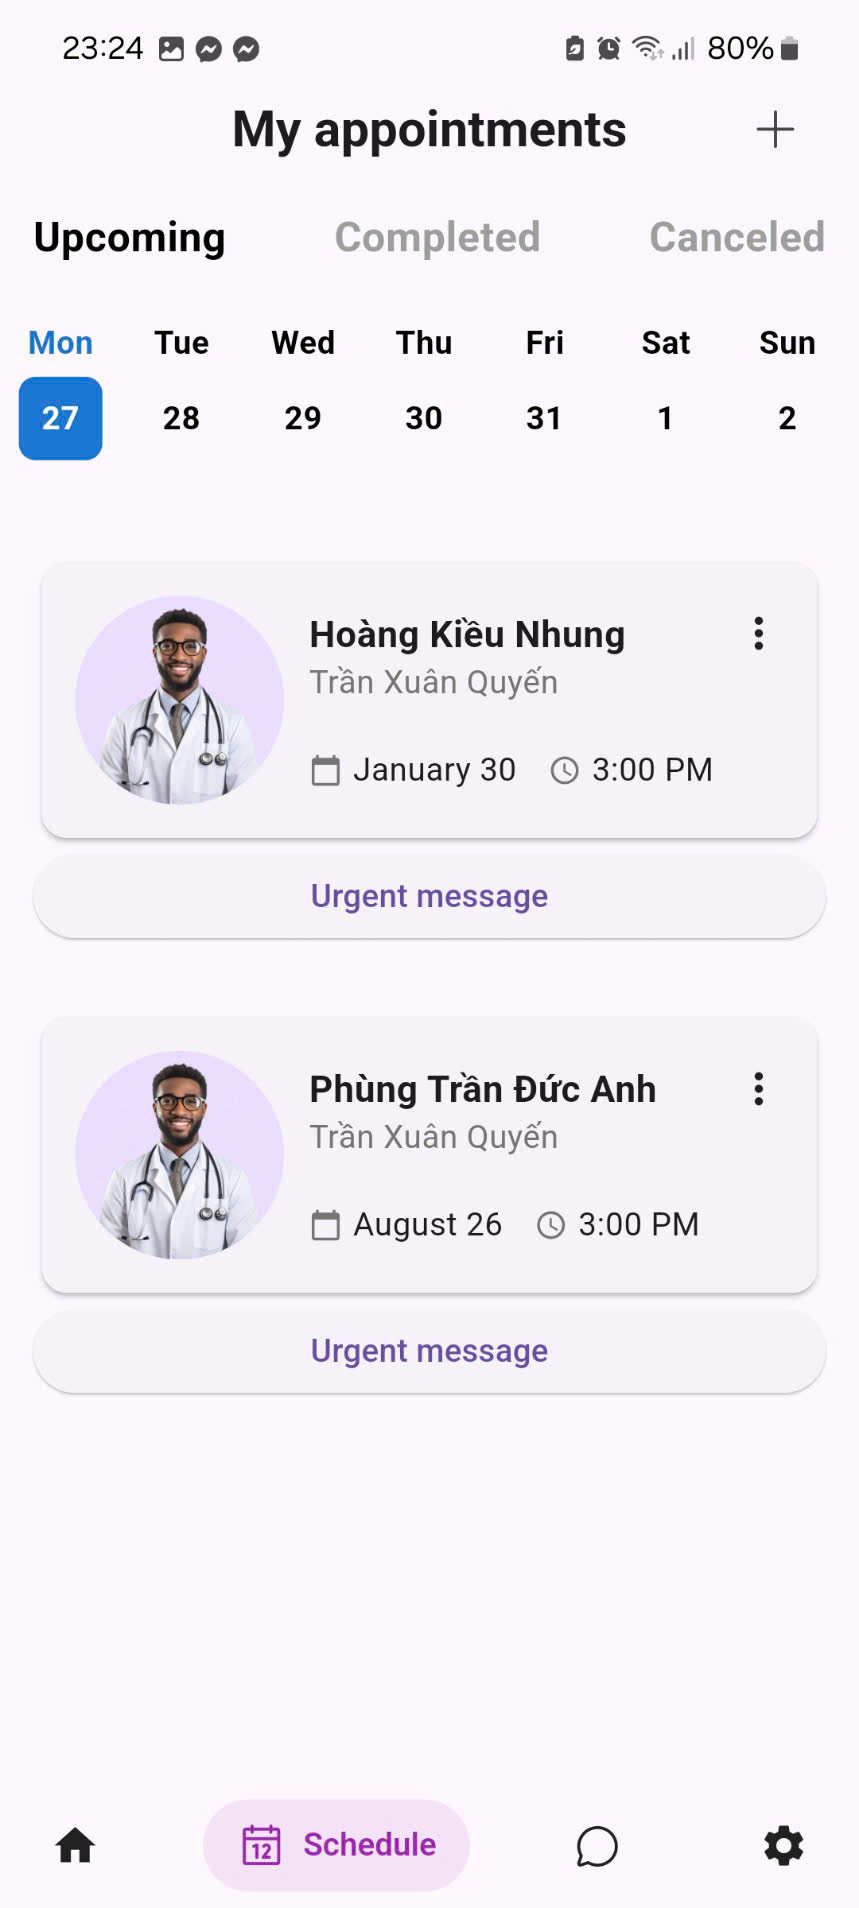
\includegraphics[width=8.5cm,height=18cm]{Images/AppUI/scheduleUpComing.jpg}
	\caption[Giao diện quản lý lịch của bác sĩ]{\bfseries \fontsize{12pt}{0pt}\selectfont Giao diện quản lý lịch của bác sĩ}
	\label{scheduleDoctor}
\end{figure}
Giao diện quản lý lịch của bác sĩ được chia thành ba tab chính: \textbf{Upcoming}, \textbf{Completed}, và \textbf{Canceled}. Tab \textbf{Upcoming} hiển thị danh sách các cuộc hẹn sắp tới với thông tin chi tiết như tên bệnh nhân, ngày và giờ hẹn, cùng nút "Urgent message" để liên lạc khẩn cấp khi cần thiết.

Sang giao diện đặt lịch:
\begin{figure}[H]
	\centering
	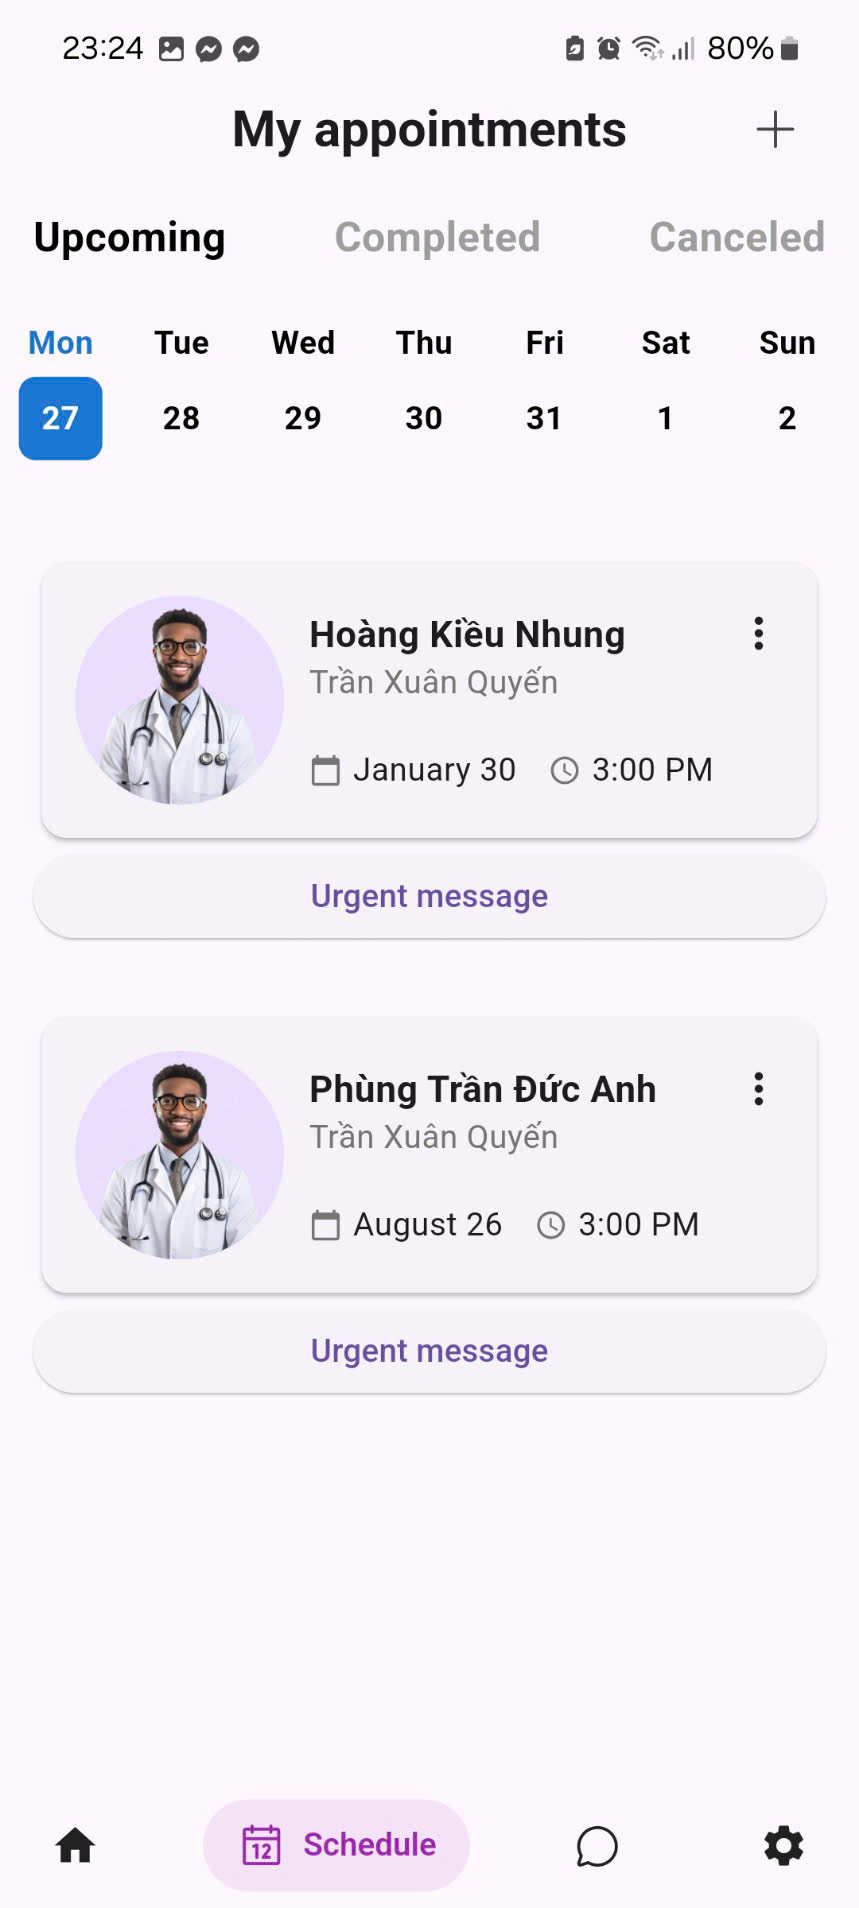
\includegraphics[width=8.5cm,height=18cm]{Images/AppUI/scheduleUpComing.jpg}
	\caption[Giao diện quản lý lịch của bác sĩ]{\bfseries \fontsize{12pt}{0pt}\selectfont Giao diện quản lý lịch của bác sĩ}
	\label{scheduleDoctor}
\end{figure}
Giao diện quản lý lịch của bác sĩ được chia thành ba tab chính: \textbf{Upcoming}, \textbf{Completed}, và \textbf{Canceled}. Tab \textbf{Upcoming} hiển thị danh sách các cuộc hẹn sắp tới với thông tin chi tiết như tên bệnh nhân, ngày và giờ hẹn, cùng nút "Urgent message" để liên lạc khẩn cấp khi cần thiết. 


\begin{figure}[H]
	\centering
	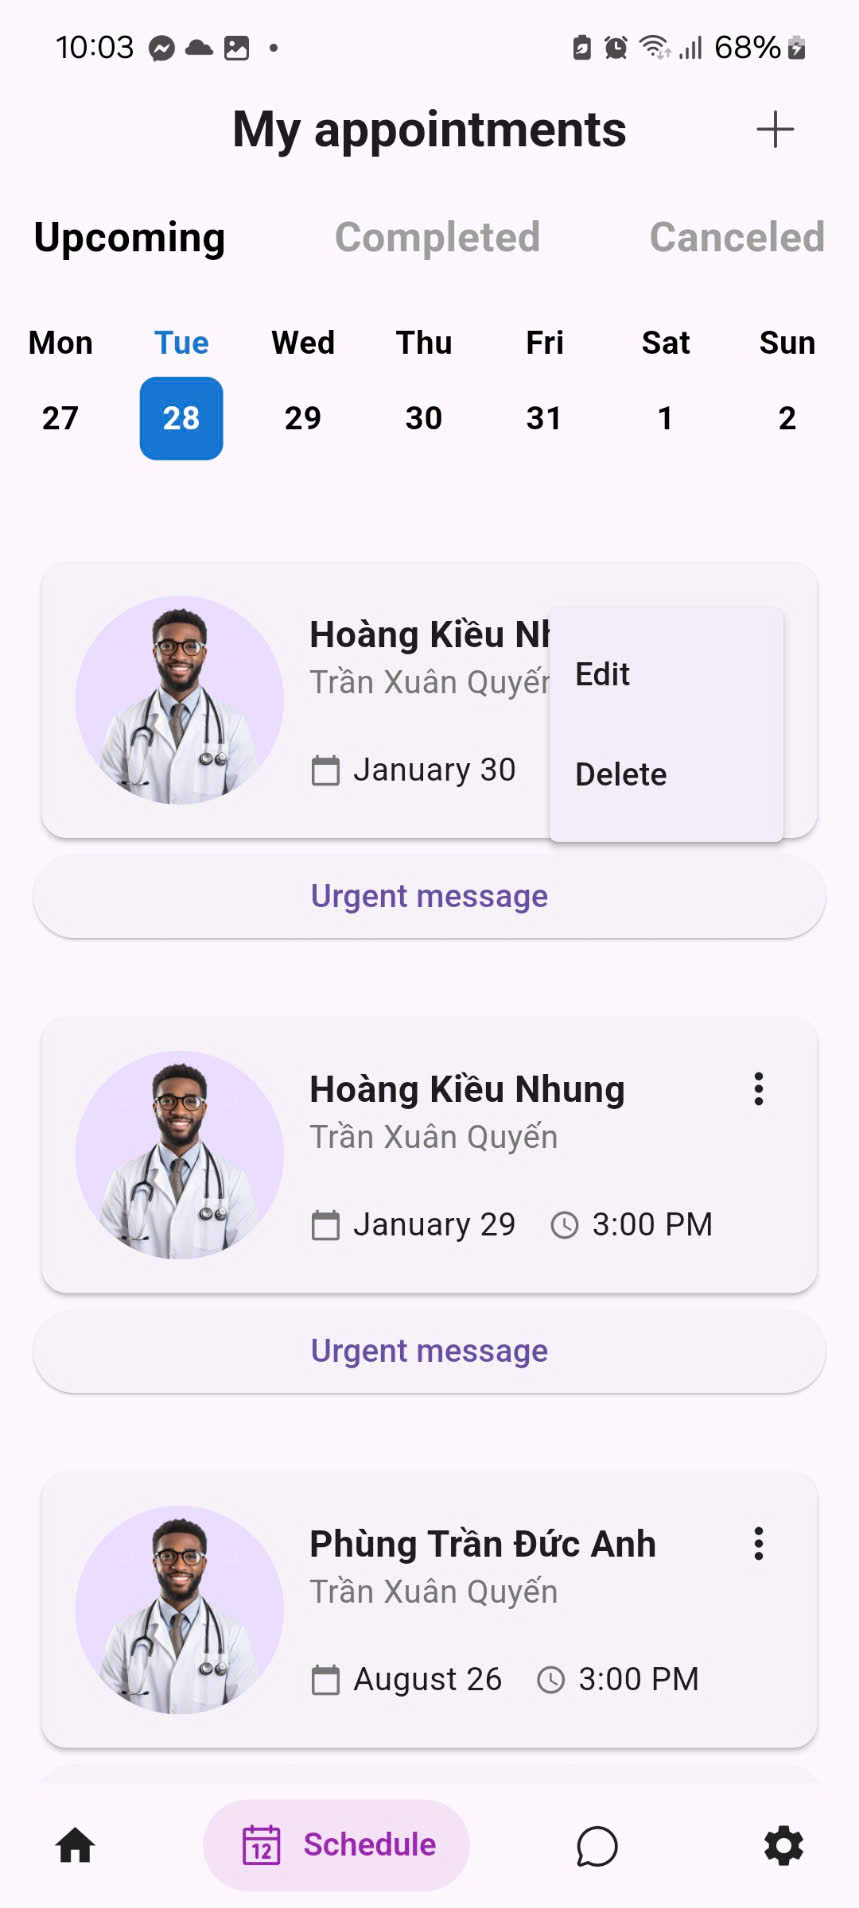
\includegraphics[width=8.5cm,height=18cm]{Images/AppUI/optionSchedule.jpg}
	\caption[Tùy chọn hủy lịch hẹn trong tab Upcoming]{\bfseries \fontsize{12pt}{0pt}\selectfont Tùy chọn hủy lịch hẹn trong tab Upcoming}
	\label{upcomingOptions}
\end{figure}
Trong tab \textbf{Upcoming}, mỗi cuộc hẹn đều có biểu tượng dấu ba chấm ở góc phải, cho phép bác sĩ truy cập vào các tùy chọn bổ sung. Một trong số đó là chức năng \textbf{Hủy lịch hẹn}. Khi nhấn vào tùy chọn này, một cửa sổ mới sẽ xuất hiện, yêu cầu bác sĩ nhập lý do hủy lịch.

\begin{figure}[H]
	\centering
	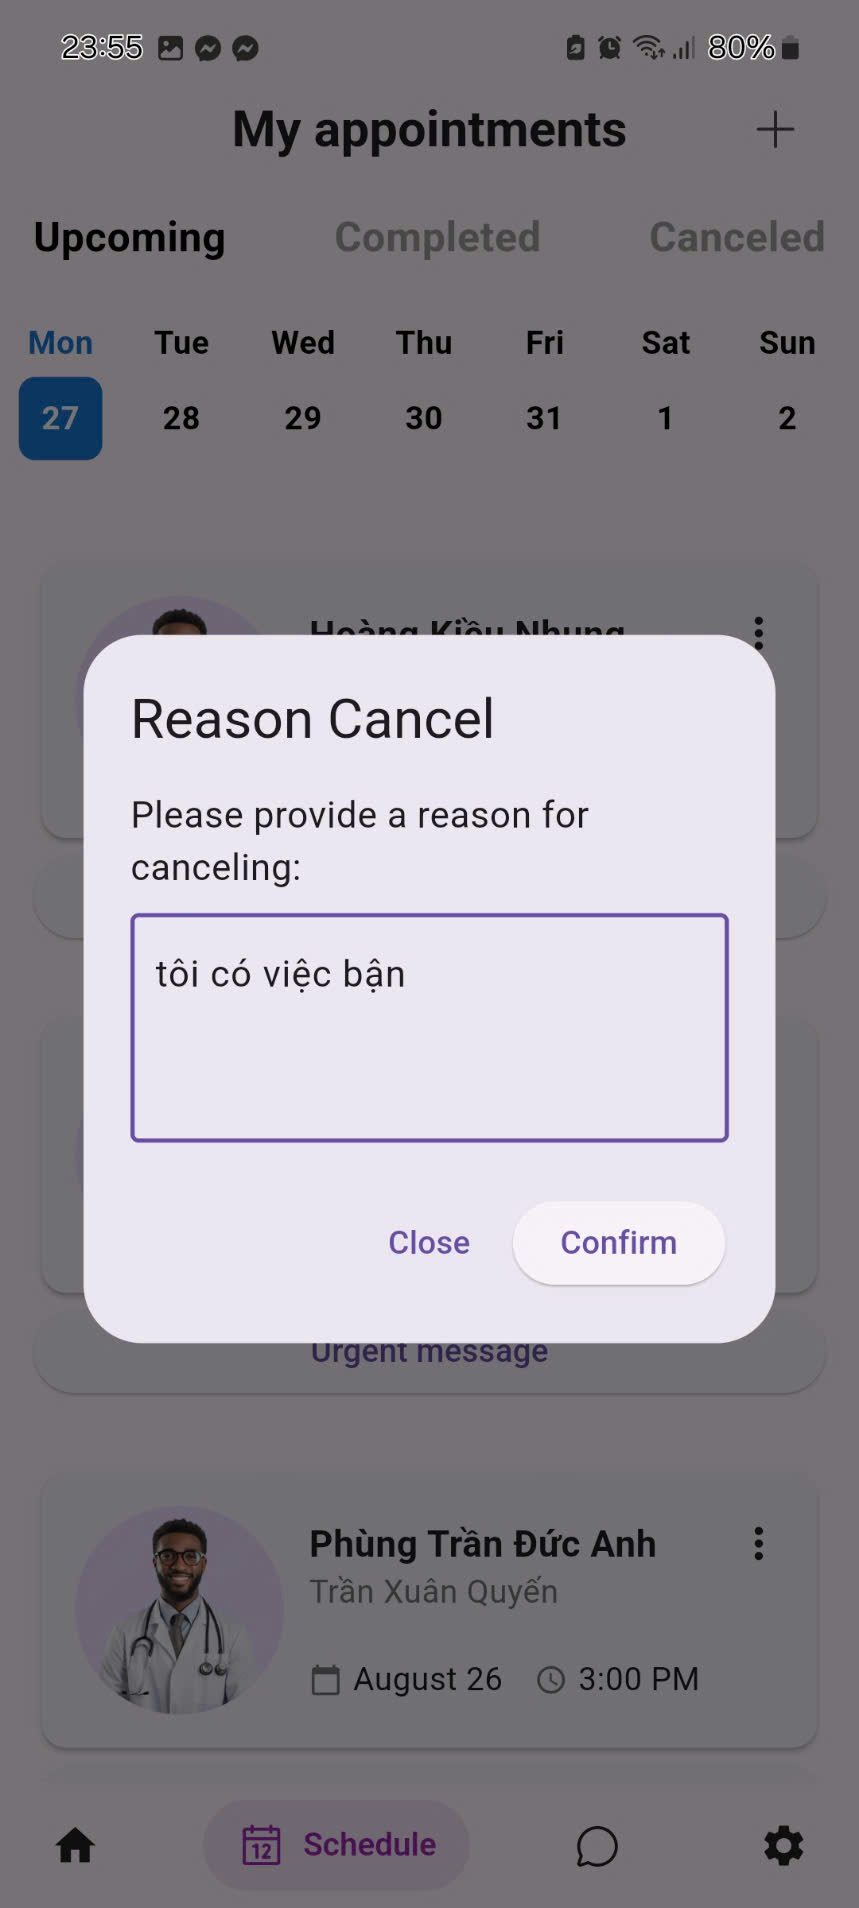
\includegraphics[width=8.5cm,height=18cm]{Images/AppUI/cancelledSchedule.jpg}
	\caption[Giao diện nhập lý do hủy lịch hẹn]{\bfseries \fontsize{12pt}{0pt}\selectfont Giao diện nhập lý do hủy lịch hẹn}
	\label{cancelAppointment}
\end{figure}
Giao diện nhập lý do hủy lịch hẹn cung cấp một ô nhập liệu để bác sĩ điền thông tin giải thích lý do hủy cuộc hẹn. Phía dưới là hai nút chức năng:
\begin{itemize}
	\item \textbf{Cancel Appointment}: Xác nhận hủy lịch hẹn sau khi lý do được nhập.
	\item \textbf{Close}: Đóng cửa sổ mà không thực hiện thay đổi.
\end{itemize}
Chức năng này đảm bảo bác sĩ có thể quản lý lịch hẹn linh hoạt, đồng thời cung cấp thông tin rõ ràng cho bệnh nhân về lý do hủy lịch.


Tab \textbf{Completed} tập hợp các cuộc hẹn đã hoàn thành. Khi nhấn vào một mục trong danh sách, bác sĩ sẽ được chuyển đến cửa sổ chi tiết, hiển thị thông tin bệnh nhân như tên, tuổi, giới tính, và số điện thoại, cùng với các tùy chọn thao tác như nhập thông tin chẩn đoán và tạo lịch tái khám. Tab \textbf{Canceled} cho phép bác sĩ theo dõi các cuộc hẹn đã bị hủy, hỗ trợ việc quản lý lịch sử làm việc dễ dàng hơn.

\begin{figure}[H]
	\centering
	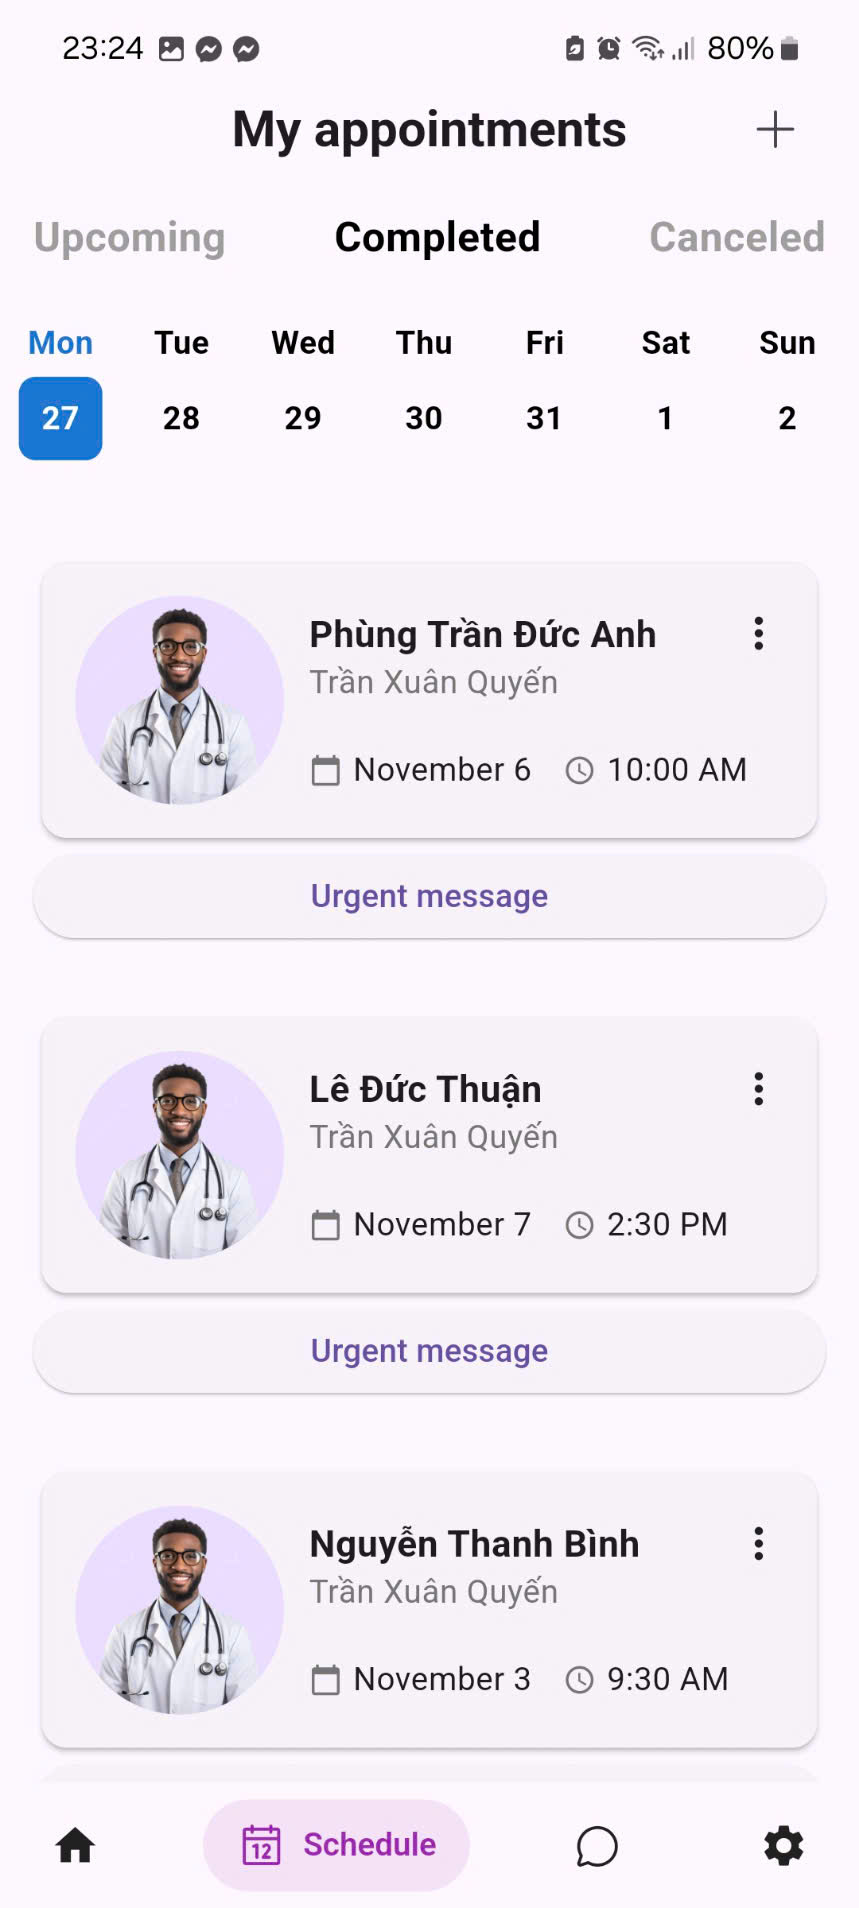
\includegraphics[width=8.5cm,height=18cm]{Images/AppUI/scheduleCompleted.jpg}
	\caption[Chi tiết thông tin bệnh nhân từ lịch đã hoàn thành]{\bfseries \fontsize{12pt}{0pt}\selectfont Chi tiết thông tin bệnh nhân từ lịch đã hoàn thành}
	\label{patientInfo}
\end{figure}
Khi truy cập vào thông tin chi tiết từ tab \textbf{Completed}, bác sĩ sẽ thấy toàn bộ thông tin về bệnh nhân, bao gồm tên, tuổi, giới tính, và số điện thoại. Bên dưới là các nút chức năng như:
\begin{itemize}
	\item \textbf{Chẩn đoán}: Cho phép bác sĩ nhập hoặc chỉnh sửa thông tin chẩn đoán cho bệnh nhân.
	\item \textbf{Tạo lịch tái khám}: Hỗ trợ bác sĩ đặt lịch tái khám mới với giao diện chọn ngày và giờ trực quan.
	\item \textbf{Đóng cửa sổ}: Kết thúc thao tác và quay lại danh sách.
\end{itemize}

\begin{figure}[H]
	\centering
	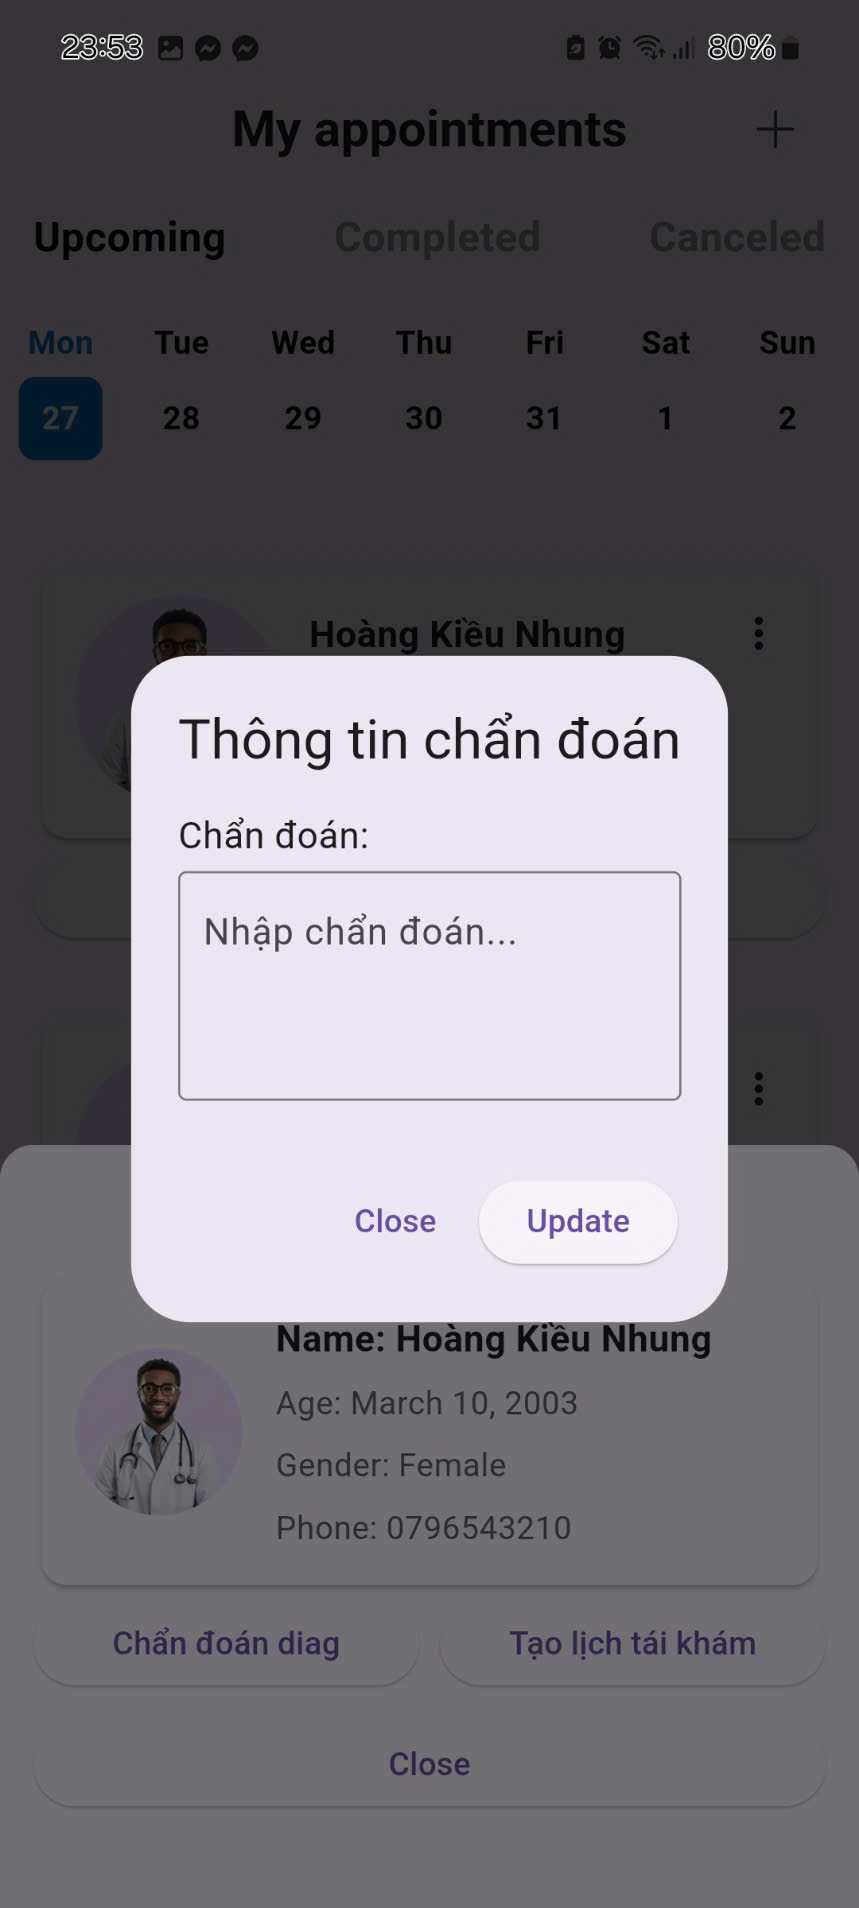
\includegraphics[width=8.5cm,height=18cm]{Images/AppUI/blockInputDIag.jpg}
	\caption[Cửa sổ cập nhật thông tin chẩn đoán]{\bfseries \fontsize{12pt}{0pt}\selectfont Cửa sổ cập nhật thông tin chẩn đoán}
	\label{diagnosisUpdate}
\end{figure}
Giao diện cập nhật chẩn đoán cung cấp một ô nhập liệu để bác sĩ thêm hoặc chỉnh sửa nội dung chẩn đoán, đi kèm nút \textbf{Update} để lưu thông tin mới.

\begin{figure}[H]
	\centering
	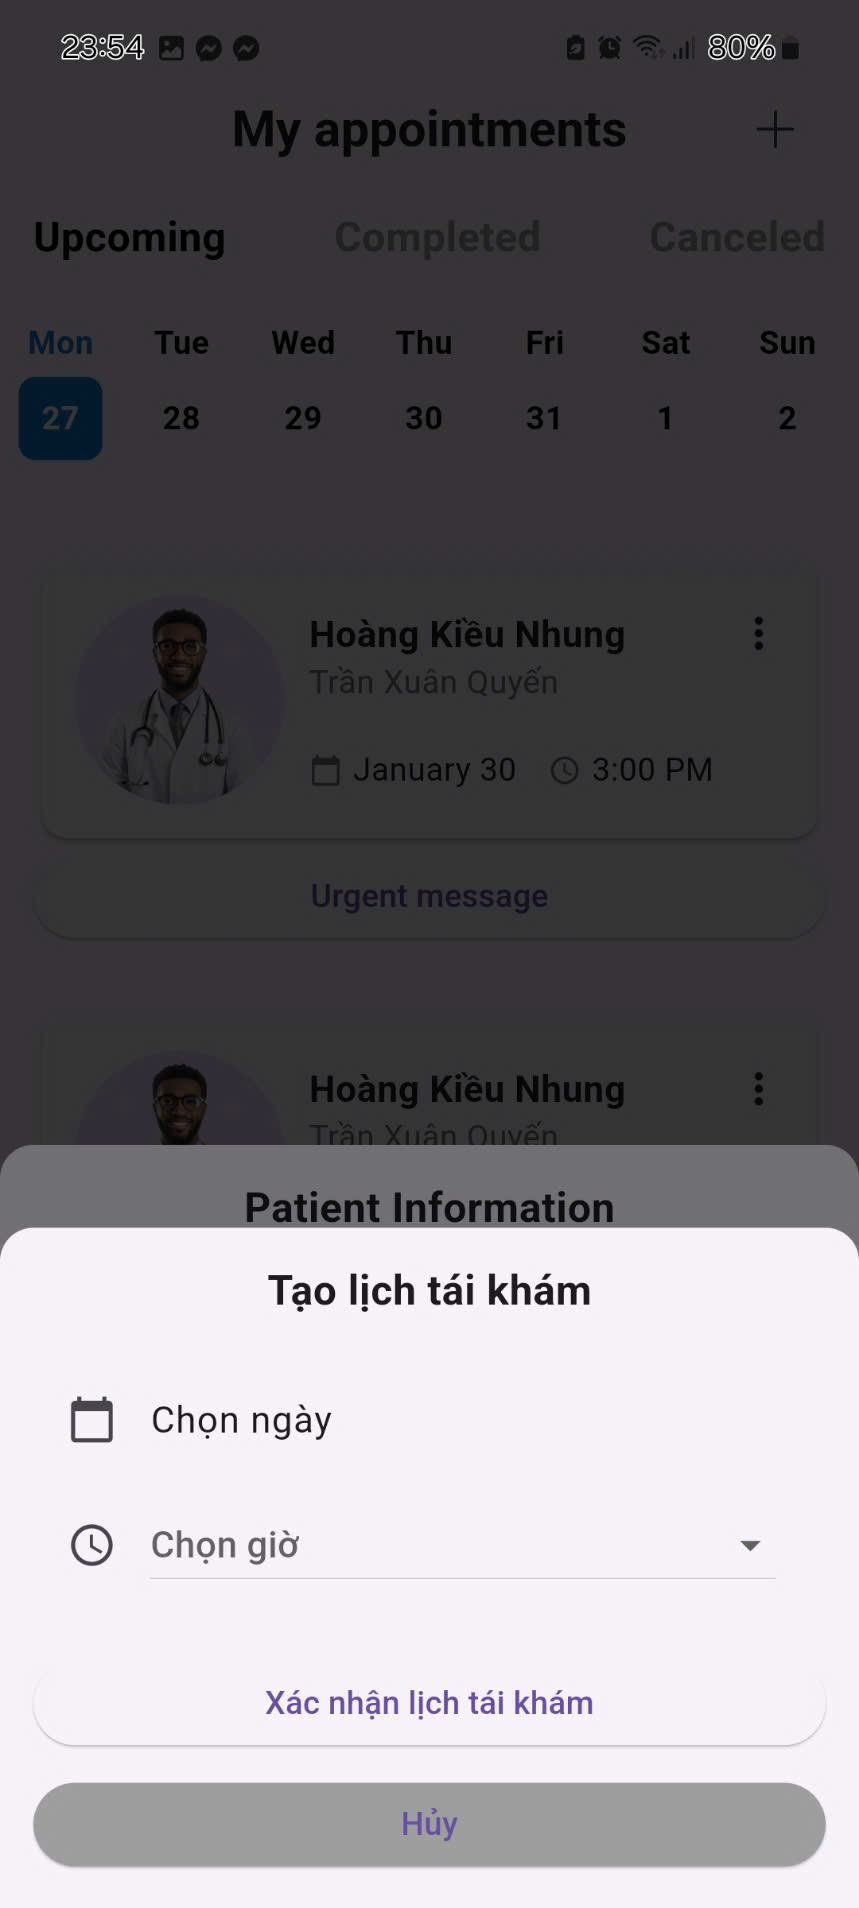
\includegraphics[width=8.5cm,height=18cm]{Images/AppUI/repickSchedule2.jpg}
	\caption[Cửa sổ tạo lịch tái khám]{\bfseries \fontsize{12pt}{0pt}\selectfont Cửa sổ tạo lịch tái khám}
	\label{reschedule}
\end{figure}
Giao diện đặt lịch tái khám cho phép bác sĩ chọn ngày và giờ, sau đó xác nhận bằng nút \textbf{Xác nhận lịch tái khám}. Điều này giúp đảm bảo việc quản lý các cuộc hẹn diễn ra mượt mà và hiệu quả.

\begin{figure}[H]
	\centering
	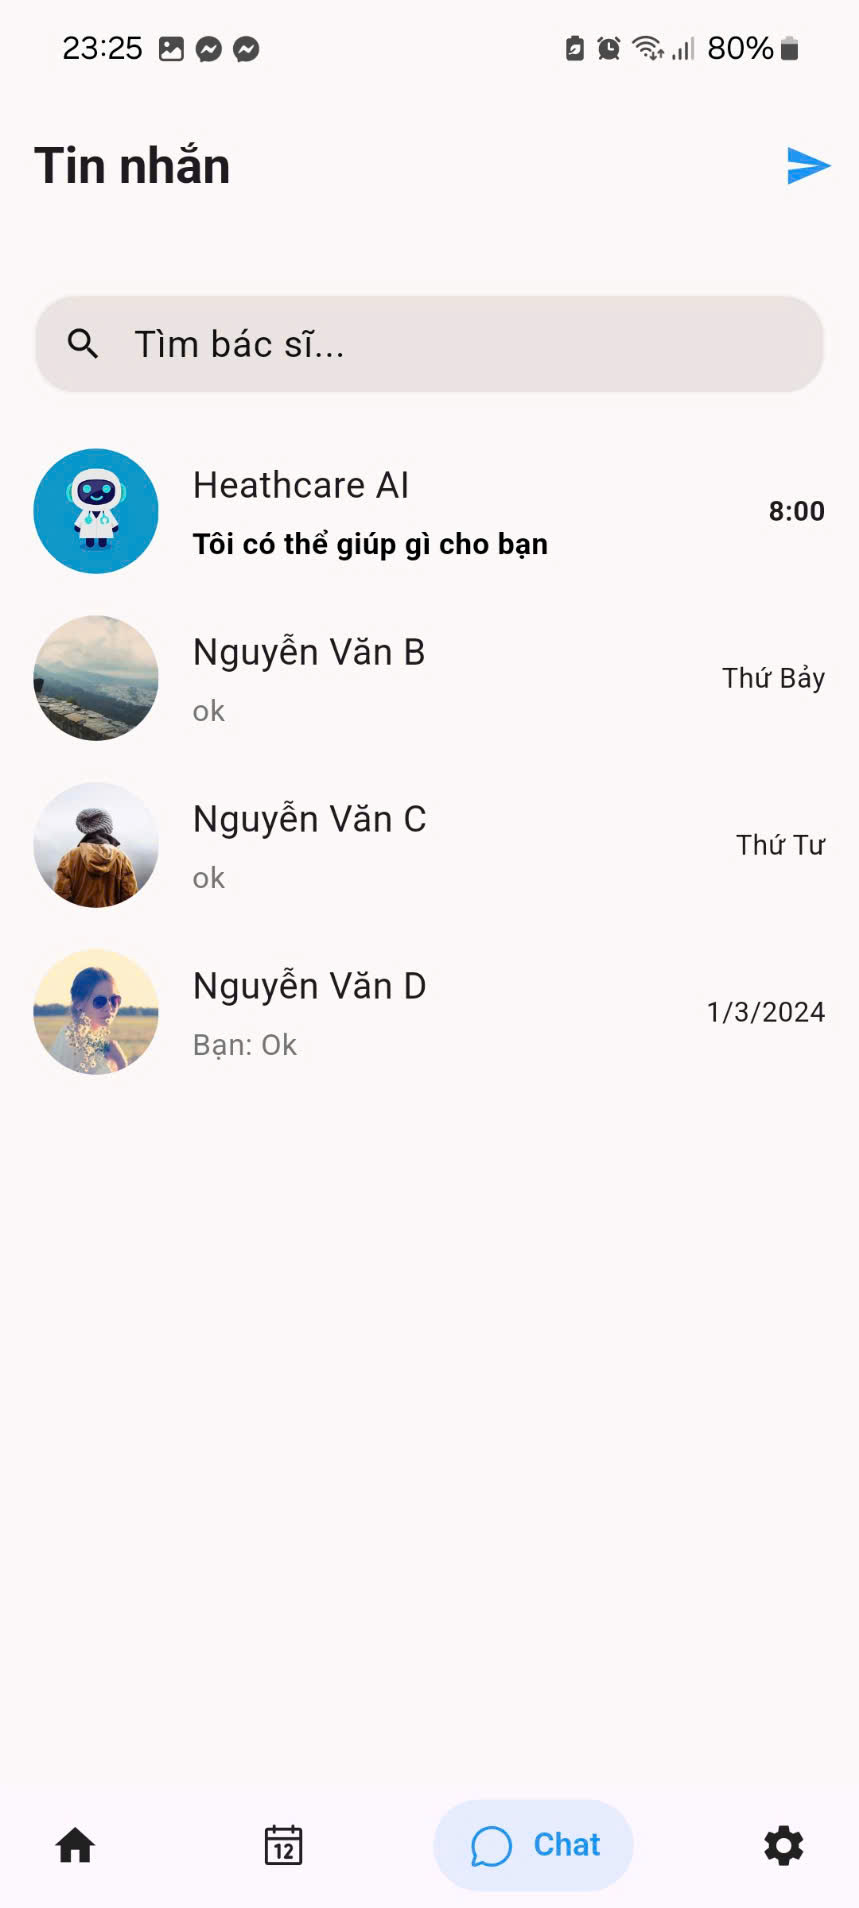
\includegraphics[width=8.5cm,height=18cm]{Images/AppUI/chatDoctor.jpg}
	\caption[Giao diện trang hội thoại]{\bfseries \fontsize{12pt}{0pt}\selectfont Giao diện trang hội thoại}
	\label{chat}
\end{figure}
Giao diện trên thuộc màn hình của bác sĩ, được thiết kế để tạo cuộc hội thoại giữa bác sĩ và bệnh nhân. Tại đây, bác sĩ có thể dễ dàng tìm kiếm tên bệnh nhân hoặc truy cập nhanh các cuộc hội thoại thông qua danh sách hiển thị ở giữa màn hình. Mỗi cuộc hội thoại đều đi kèm với tên người liên hệ, tin nhắn gần nhất, và thời gian trao đổi, giúp bác sĩ nhanh chóng xác định nội dung cần trao đổi.

\begin{figure}[H]
	\centering
	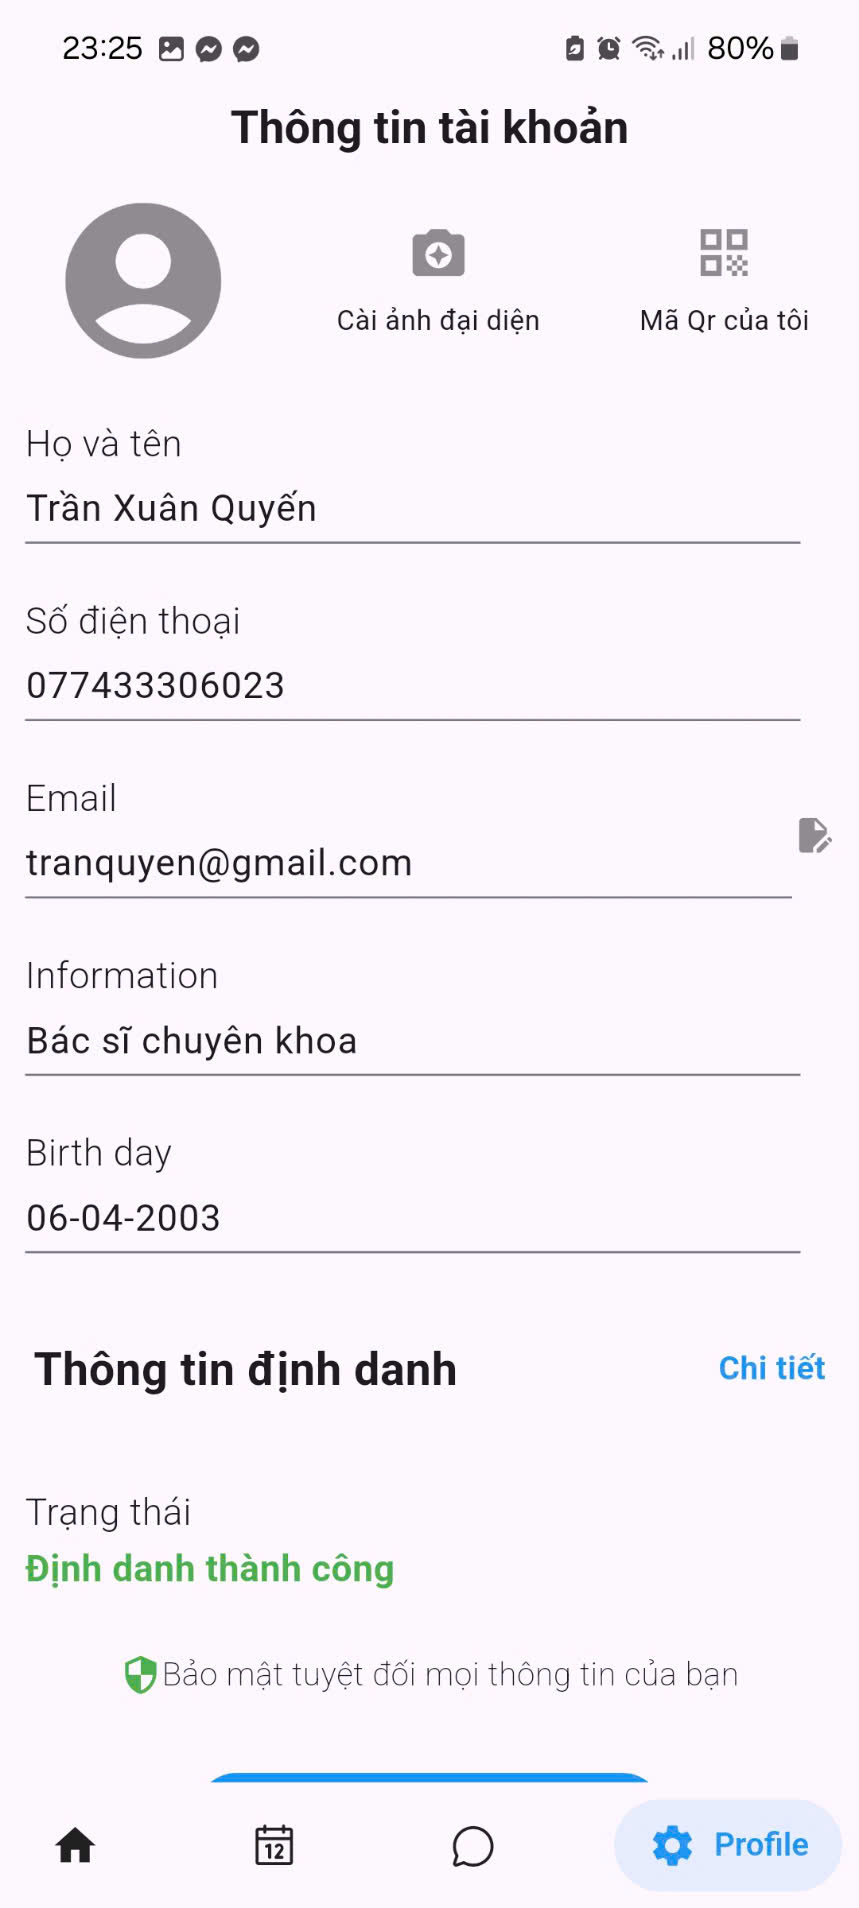
\includegraphics[width=8.5cm,height=18cm]{Images/AppUI/infoDoctor.jpg}
	\caption[Giao diện màn thông tin của bác sĩ]{\bfseries \fontsize{12pt}{0pt}\selectfont Giao diện màn thông tin của bác sĩ}
	\label{infoDoctor}
\end{figure}

Trong phần "Profile" dành cho bác sĩ, giao diện cung cấp đầy đủ các chi tiết cơ bản như họ và tên, số điện thoại, email, và ngày sinh của người dùng. Ngoài ra, chức năng hiển thị rõ vai trò chuyên môn của bác sĩ, chẳng hạn như "Bác sĩ chuyên khoa". Một điểm nổi bật là tính năng định danh tài khoản, được hiển thị với trạng thái "Định danh thành công", nhằm đảm bảo bảo mật và xác thực thông tin của bác sĩ. Giao diện trực quan, dễ sử dụng, giúp bác sĩ nhanh chóng truy cập và cập nhật thông tin cá nhân.


\begin{figure}[H]
	\centering
	
\includegraphics[width=8.5cm,height=6cm]{Images/AppUI/buttonInfoPage.png}
	\caption[Giao diện màn thông tin của bác sĩ]{\bfseries \fontsize{12pt}{0pt}\selectfont Giao diện màn thông tin của bác sĩ}
	\label{infoDoctor}
\end{figure}

Ngoài việc cung cấp các thông tin cá nhân chi tiết, phần này còn có hai nút chức năng quan trọng: "Cập nhật lại định danh" và "Đăng xuất". Nút "Cập nhật lại định danh" cho phép bác sĩ xác thực lại thông tin tài khoản để đảm bảo tính chính xác và an toàn. Trong khi đó, nút "Đăng xuất" được thiết kế với màu đỏ nổi bật, giúp bác sĩ nhanh chóng thoát khỏi tài khoản khi cần thiết. Cả hai nút đều được đặt ở vị trí dễ thấy, hỗ trợ tốt cho việc quản lý tài khoản một cách hiệu quả.
\subsubsection{Giao diện của bệnh nhân (Patient)}

\begin{figure}[H]
	\centering
	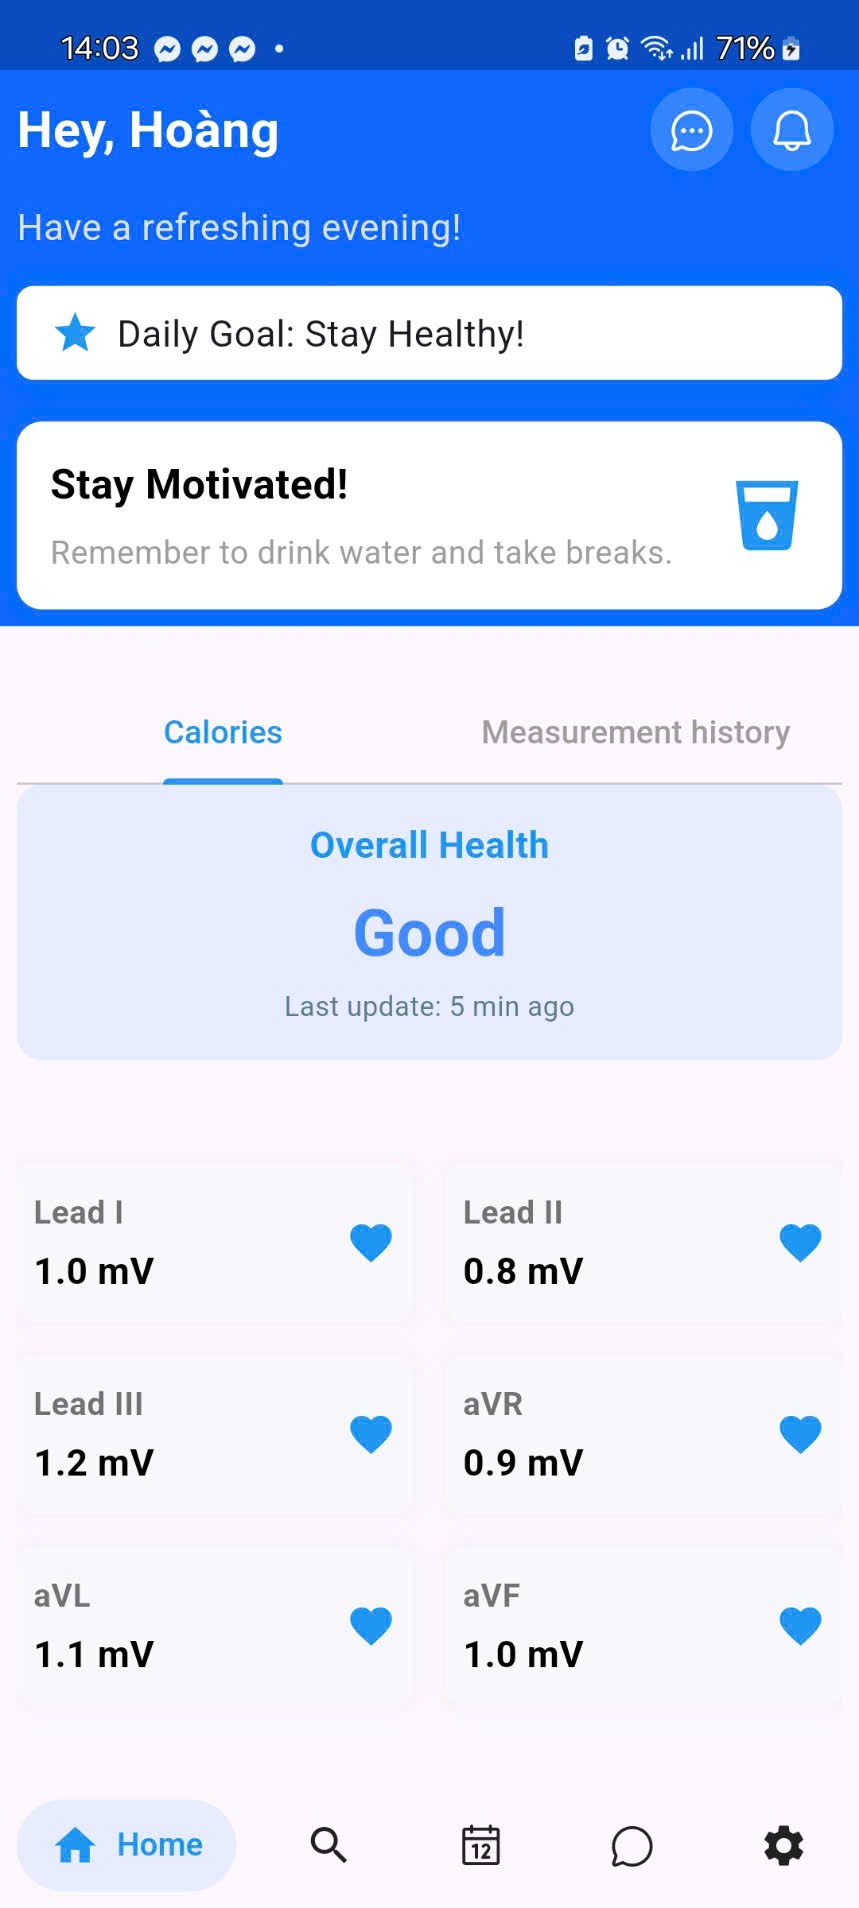
\includegraphics[width=8.5cm,height=18cm]{Images/AppUI/homePagePatient.jpg}
	\caption[Giao diện thông tin sức khỏe của bệnh nhân]{\bfseries \fontsize{12pt}{0pt}\selectfont Giao diện thông tin sức khỏe của bệnh nhân}
	\label{healthInfoPatient}
\end{figure}
Giao diện của bệnh nhân tập trung vào việc hiển thị trạng thái sức khỏe tổng quan với đánh giá "Overall Health: Good" được cập nhật gần nhất. Bên dưới là 6 số liệu liên quan đến điện tim, được trình bày rõ ràng và dễ hiểu. Những số liệu này giúp bệnh nhân theo dõi tình trạng sức khỏe tim mạch của mình một cách trực quan và chi tiết.


\begin{figure}[H]
	\centering
	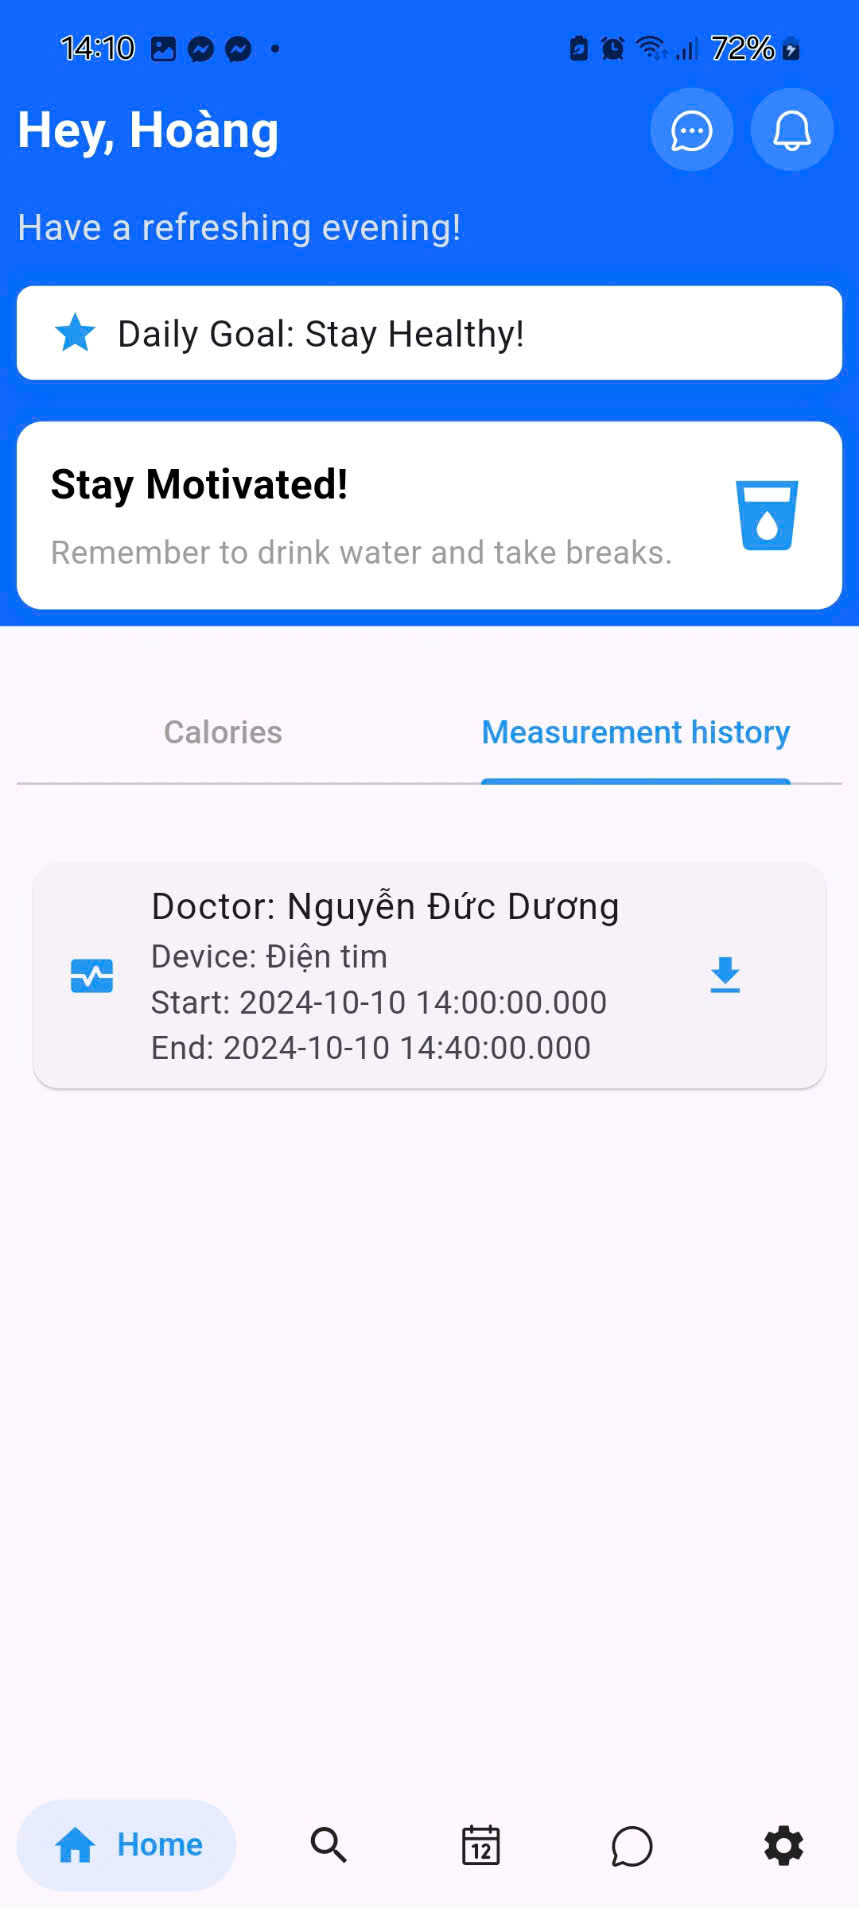
\includegraphics[width=8.5cm,height=18cm]{Images/AppUI/homePagePatient2.jpg}
	\caption[Giao diện lịch sử đo của bệnh nhân]{\bfseries \fontsize{12pt}{0pt}\selectfont Giao diện lịch sử đo của bệnh nhân}
	\label{measurementHistory}
\end{figure}
	Ở Tab \textbf{Measurement history}, cung cấp cho bệnh nhân lịch sử các lần đo trước đo với tên bác sĩ cùng với đó là thời gian bắt đầu đo và thời gian kết thúc đo, tên thiết bị đo.

\begin{figure}[H]
		\centering
		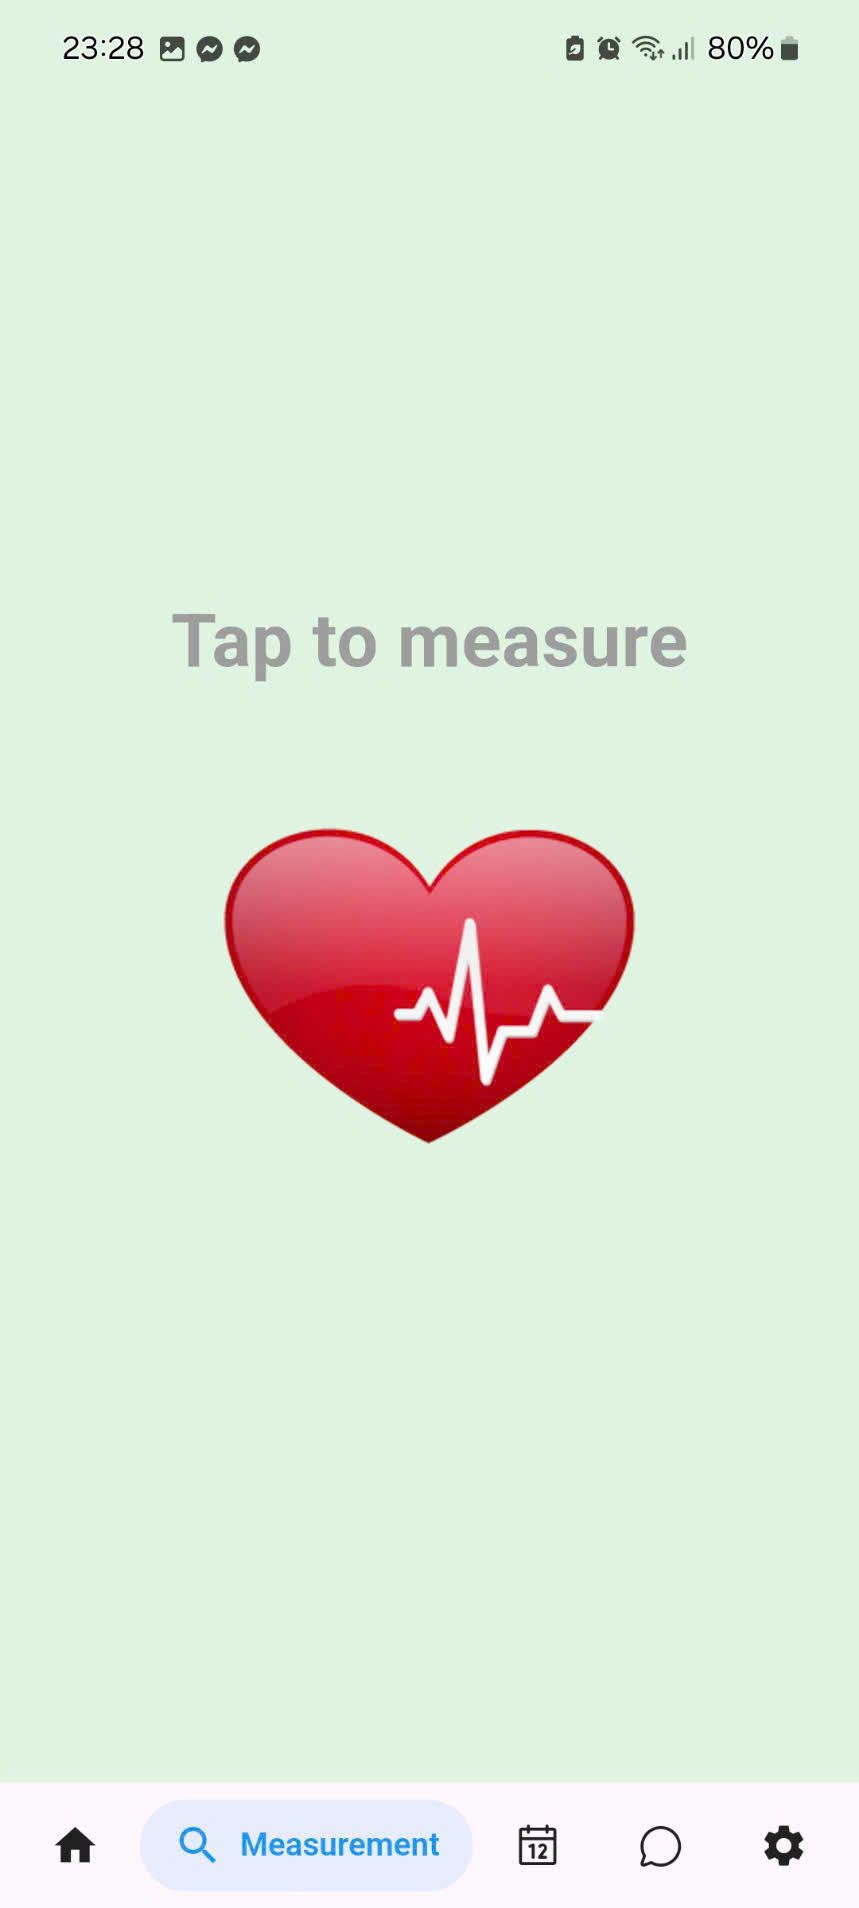
\includegraphics[width=8.5cm,height=18cm]{Images/AppUI/measure.jpg}
		\caption[Giao diện đo tín hiệu điện tim của bệnh nhân]{\bfseries \fontsize{12pt}{0pt}\selectfont Giao diện đo tin hiệu điện tim của bệnh nhân}
		\label{measurement}
\end{figure}
	Đây là giao diện phần Measurement khi bệnh nhân muốn đo tín hiệu điện tim, khi click vào hình trái tim, thiết bị sẽ bắt đầu đo và kết quả sẽ được hiển thị trên màn hình điện thoại của bệnh nhân.

	Giao diện phần đặt lịch Schedules, chủ yếu vẫn khá giống giao diện bên phần của bác sĩ, có sự khác biệt khi click vào nút "+" ở bên trên góc phải, sẽ xuất hiện màn hình lựa chọn
\begin{figure}[H]
		\centering
		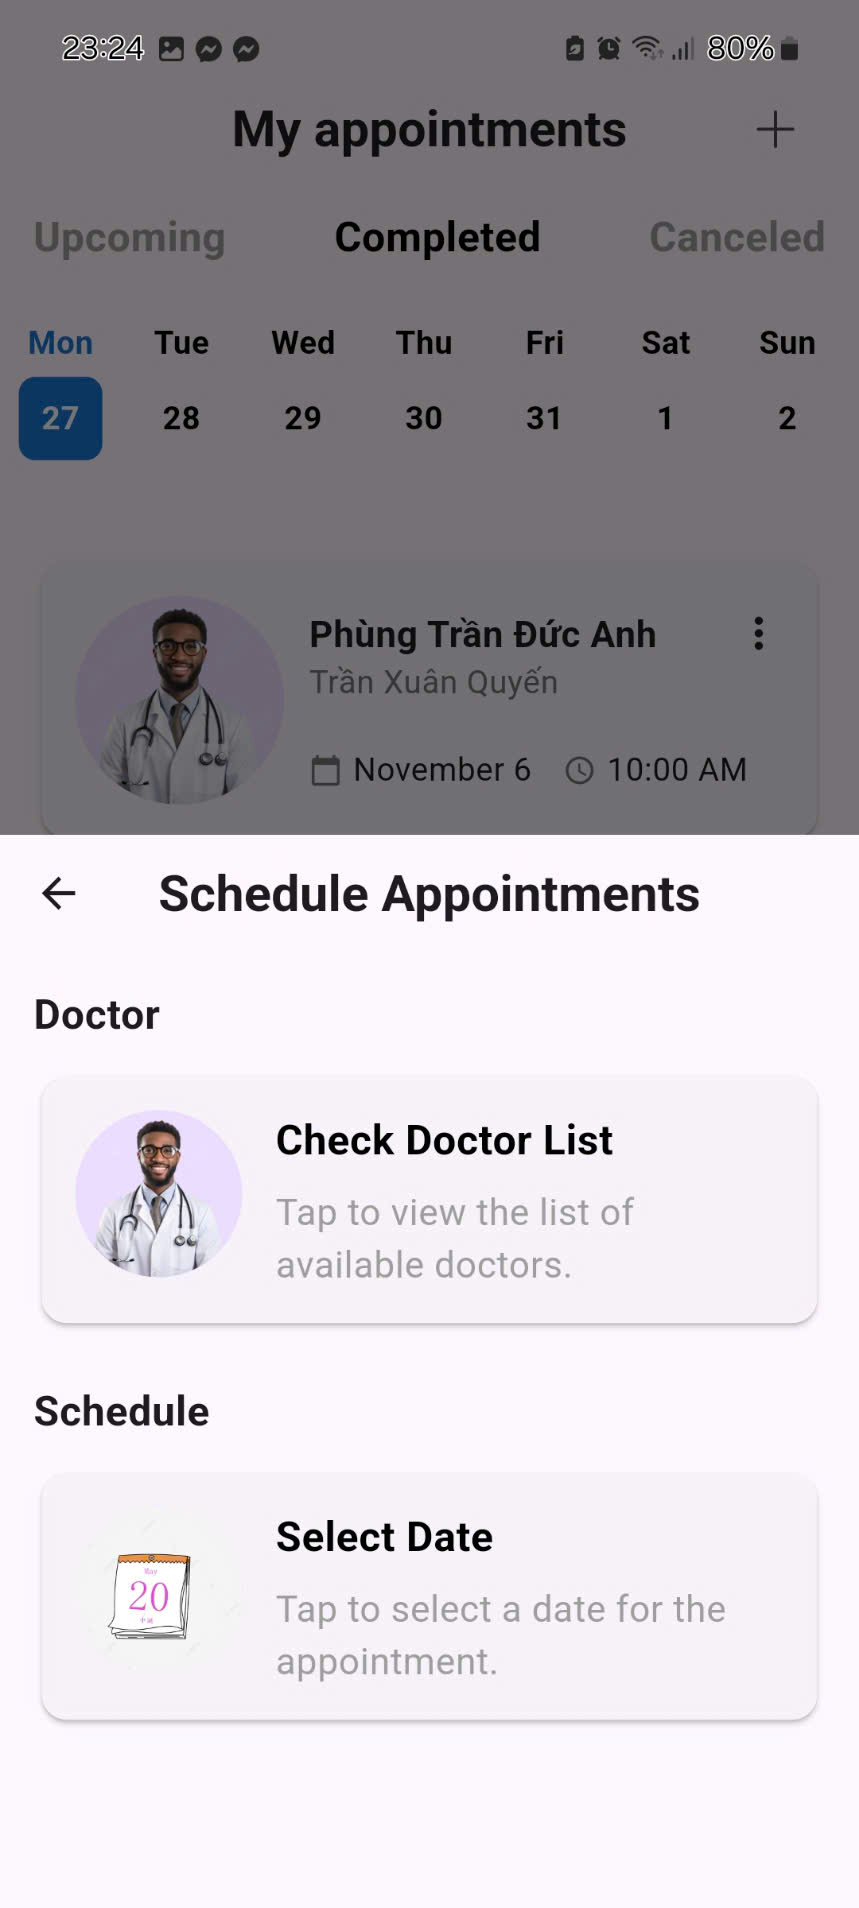
\includegraphics[width=8.5cm,height=18cm]{Images/AppUI/scheduleChoice.jpg}
		\caption[Giao diện lựa chọn kiểu đặt lịch cho bệnh nhân]{\bfseries \fontsize{12pt}{0pt}\selectfont Giao diện lựa chọn kiểu đặt lịch của bệnh nhân}
		\label{scheduleChoice}
\end{figure}
	Với lựa chọn đầu tiên là chọn Bác sĩ trước, bệnh nhân có thể lựa chọn bác sĩ mình muốn đặt lịch trước rồi mới cần chọn lịch dựa trên những lịch đang rảnh của bác sĩ

\begin{figure}[H]
	\centering
	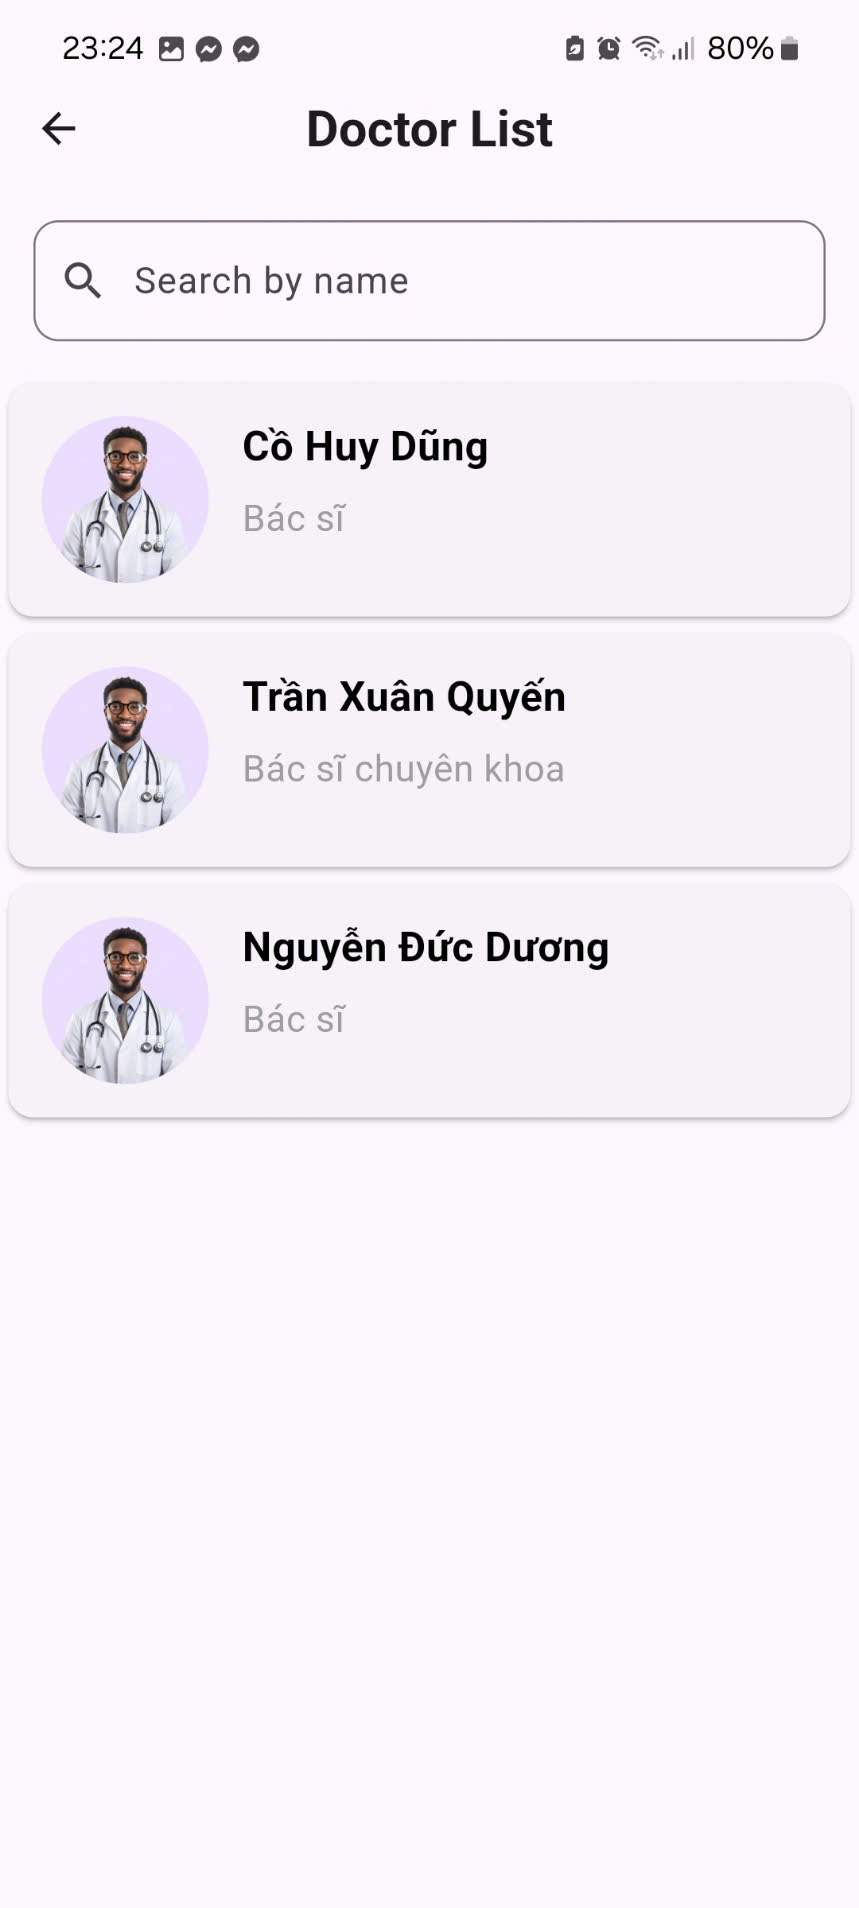
\includegraphics[width=8.5cm,height=18cm]{Images/AppUI/pickDoctor.jpg}
	\caption[Giao diện lựa chọn bác sĩ]{\bfseries \fontsize{12pt}{0pt}\selectfont Giao diện lựa chọn bác sĩ}
	\label{DoctorList}
\end{figure}
\begin{figure}[H]
	\centering
	\includegraphics[width=8.5cm,height=18cm]{Images/AppUI/selectTimeWithDoctorPick.jpg}
	\caption[Giao diện chọn thời gian tương ứng với bác sĩ đã chọn trước đó]{\bfseries \fontsize{12pt}{0pt}\selectfont Giao diện chọn thời gian tương ứng với bác sĩ đã chọn trước đó}
	\label{TimePickWithDoctor}
\end{figure}

Khi đã chọn xong sẽ hiển thị Popup xác nhận đặt lịch của bệnh nhân
\begin{figure}[H]
	\centering
	\includegraphics[width=8.5cm,height=18cm]{Images/AppUI/firmPicker.jpg}
	\caption[Popup xác nhận đặt lịch]{\bfseries \fontsize{12pt}{0pt}\selectfont Popup xác nhận đặt lịch}
	\label{TimePickWithDoctor}
\end{figure}

	Với lựa chọn thứ 2 là chọn thời gian trước, bệnh nhân sẽ đặt thời gian rảnh trước và màn hình sẽ hiển thị ra các bác sĩ đang rảnh trong thời gian đó để bệnh nhân có thể lựa chọn. Quy trình xác nhận đặt lịch tương tự như phần bên trên.

Khi đặt lịch thành công, sẽ có thông báo trả về ở phần Thông báo của cả bệnh nhân lẫn bác sĩ.
\begin{figure}[H]
	\centering
	\includegraphics[width=8.5cm,height=18cm]{Images/AppUI/noti.jpg}
	\caption[Giao diện thông báo đặt lịch thành công]{\bfseries \fontsize{12pt}{0pt}\selectfont Giao diện thông báo đặt lịch thành công}
	\label{TimePickWithDoctor}
\end{figure}
Về giao diện phần Hội thoại và Thông tin cá nhân sẽ được thiết kế giống với phần giao diện bên phía bác sĩ.

\begin{figure}[H]
	\centering
	\includegraphics[width=8.5cm,height=18cm]{Images/AppUI/infoPatient.jpg}
	\caption[Giao diện thông tin cá nhân của bệnh nhân]{\bfseries \fontsize{12pt}{0pt}\selectfont Giao diện thông tin cá nhân của bệnh nhân}
	\label{TimePickWithDoctor}
\end{figure}
	\subsection{Thiết kế các chức năng}

	\subsubsection{Thiết kế các API cần thiết}


	\begin{enumerate}[a)]
		\item API xác minh tài khoản
	
		\begin{xltabular}{\textwidth}{
		  | >{\raggedright\arraybackslash}m{4.6cm}
		  | >{\centering\arraybackslash}m{2.8cm}
		  | >{\raggedright\arraybackslash}X |
		  }
		  \caption{\bfseries \fontsize{12pt}{0pt}\selectfont Bảng API xác minh tài khoản}
		  \label{table_api_auth}
		  \\
		  \hline
		  \bfseries Đường dẫn    &\bfseries Phương thức    &\bfseries Mô tả\\ \hline
		  api/ecg/auth/create-account   &   POST  & Tạo mới tài khoản người dùng \\ \hline
		  api/ecg/auth/login   &    POST    & Đăng nhập vào hệ thống \\ \hline
		  api/ecg/auth/logout   &    POST    & Đăng xuất khỏi hệ thống \\ \hline
		\end{xltabular}
	  
		\item API quản lý người dùng trong hệ thống
		\begin{xltabular}{\textwidth}{
		  | >{\raggedright\arraybackslash}m{4.6cm}
		  | >{\centering\arraybackslash}m{2.8cm}
		  | >{\raggedright\arraybackslash}X |
		  }
		  \caption{\bfseries \fontsize{12pt}{0pt}\selectfont Bảng API quản lý người dùng trong hệ thống}
		  \label{table_api_user}
		  \\
		  \hline
		  \bfseries Đường dẫn    &\bfseries Phương thức    &\bfseries Mô tả\\ \hline
		  api/ecg/users   &   GET  &  Tra cứu danh sách tất cả người dùng trong hệ thống\\  \hline
		  api/ecg/users/doctors   &   GET  &  Tra cứu danh sách toàn bộ bác sĩ trong hệ thống \\  \hline
		  api/ecg/users/:id   &   GET  &  Tra cứu dữ liệu người dùng cụ thể dựa trên id tương ứng \\  \hline
		  api/ecg/users/data/patient-data   &   GET  &  Tra cứu danh sách các bệnh nhân đang được theo dõi của bác sĩ cụ thể \\  \hline
		  api/ecg/users/data/doctor-id   &   GET  &  Tra cứu thông tin của bác sĩ phụ trách bệnh nhân \\  \hline
		  api/ecg/users/   &   PUT  &  Chỉnh sửa thông tin người dùng \\  \hline
		  api/ecg/users/:userId  &   DELETE  &  Xóa người dùng cụ thể dựa trên id tương ứng \\  \hline
		\end{xltabular}
	  
	  \item API quản lý thiết bị y tế
	  \begin{xltabular}{\textwidth}{
		| >{\raggedright\arraybackslash}m{4.8cm}
		| >{\centering\arraybackslash}m{2.8cm}
		| >{\raggedright\arraybackslash}X |
		}
		\caption{\bfseries \fontsize{12pt}{0pt}\selectfont Bảng API quản lý thiết bị y tế}
		\label{table_api_device}
		\\
		\hline
		\bfseries Đường dẫn    &\bfseries Phương thức    &\bfseries Mô tả\\ \hline
		api/ecg/device   &   GET  & Tra cứu danh sách toàn bộ thiết bị y tế trong hệ thống\\ \hline
		api/ecg/devide/:id   &    GET    & Tra cứu thông tin chi tiết của một thiết bị y tế dựa trên id tương ứng \\ \hline
		api/ecg/device/add &   POST     & Thêm mới thiết bị y tế \\ \hline
		api/ecg/device/update  &     PUT   & Cập nhật thông tin chi tiết cho thiết bị y tế cụ thể \\ \hline
		api/ecg/device/:deviceId  &     DELETE   & Xóa thiết bị y tế dựa trên id tương ứng \\ \hline
	  \end{xltabular}
	  
	  \item API quản lý dữ liệu phiên đo
	  \begin{xltabular}{\textwidth}{
		| >{\raggedright\arraybackslash}p{5cm}
		| >{\centering\arraybackslash}m{2.8cm}
		| >{\raggedright\arraybackslash}X |
		}
		\caption{\bfseries \fontsize{12pt}{0pt}\selectfont Bảng API quản lý dữ liệu phiên đo}
		\label{table_api_record}
		\\
		\hline
		\bfseries Đường dẫn    &\bfseries Phương thức    &\bfseries Mô tả \\ \hline
		 api/ecg/records   &   GET  & Tra cứu danh sách các dữ liệu phiên đo \\ \hline
		 api/ecg/records/:id   &    GET    & Tra cứu dữ liệu phiên đo cụ thể dựa theo id tương ứng \\ \hline
		 api/ecg/records/data/ doctor &   GET     & Tra cứu danh sách các dữ liệu phiên đo của bệnh nhân mà bác sĩ phụ trách \\ \hline
		 api/ecg/records/data/ patient &   GET     & Tra cứu danh sách dữ liệu các phiên đo cá nhân \\ \hline
		 api/ecg/records/   &    POST    & Tạo dữ liệu phiên đo mới \\ \hline
		 api/ecg/records/   &    PUT    & Cập nhật dữ liệu phiên đo \\ \hline
		 api/ecg/records/:recordId  &    DELETE    & Xóa dữ liệu phiên đo dựa theo id tương ứng \\ \hline
		\end{xltabular}
	  
	  
	  \item API quản lý dịch vụ lịch khám
	  \begin{xltabular}{\textwidth}{
		| >{\raggedright\arraybackslash}m{4.5cm}
		| >{\centering\arraybackslash}m{2.8cm}
		| >{\raggedright\arraybackslash}X |
		}
		\caption{\bfseries \fontsize{12pt}{0pt}\selectfont Bảng API quản lý dịch vụ lịch khám}
		\label{table_api_schedule}
		\\
		\hline
		\bfseries Đường dẫn    &\bfseries Phương thức    &\bfseries Mô tả\\ \hline
		api/ecg/schedules   &   GET  & Tra cứu danh sách tất cả lịch khám trong hệ thống \\ \hline
		api/ecg/schedules/ doctor-id  &    GET    & Tra cứu danh sách lịch khám của bác sĩ cụ thể \\ \hline
		api/ecg/schedules/ patient-id  &    GET    & Tra cứu danh sách lịch khám của bệnh nhân cụ thể \\ \hline
		api/ecg/schedules/create-by-doctor  &    POST    & Cho phép bác sĩ đặt lịch tái khám cho bệnh nhân \\ \hline
		api/ecg/schedules/create-by-patient  &    POST    & Cho phép bệnh nhân đặt lịch khám với bác sĩ \\ \hline
		api/ecg/schedules/time/ available-doctor/: schedule-time  &    GET    & Tra cứu danh sách các bác sĩ khả dụng theo thời gian đã chọn \\ \hline
		api/ecg/schedules/ available-schedule/:id  &    GET    & Tra cứu các khung giờ trống có thể đặt lịch với bác sĩ cụ thể. \\ \hline
		api/ecg/schedules/accept-schedule  &    PUT    & Chấp nhận lịch khám cụ thể \\ \hline
		api/ecg/schedules/reject-schedule/:id  &    DELETE    & Từ chối lịch khám cụ thể \\ \hline
		\end{xltabular}
	  
	  \item API liên quan đến chẩn đoán cho bệnh nhân
	  \begin{xltabular}{\textwidth}{
		| >{\raggedright\arraybackslash}m{4.5cm}
		| >{\centering\arraybackslash}m{2.8cm}
		| >{\raggedright\arraybackslash}X |
		}
		\caption{\bfseries \fontsize{12pt}{0pt}\selectfont Bảng API liên quan đến chẩn đoán cho bệnh nhân}
		\label{table_api_diagnosis}
		\\
		\hline
		\bfseries Đường dẫn    &\bfseries Phương thức    &\bfseries Mô tả\\ \hline
		api/ecg/diagnosis   &   POST  & Tạo chẩn đoán mới cho bệnh nhân \\ \hline
		api/ecg/diagnosis/ schedule/:scheduleId   &   POST  & Tra cứu thông tin chẩn đoán dựa trên id lịch khám tương ứng\\ \hline
		api/ecg/diagnosis/update   &   POST  & Cập nhật thông tin chẩn đoán \\ \hline
		\end{xltabular}
	  
	  
	  \item API liên quan đến thông báo về lịch khám
	  \begin{xltabular}{\textwidth}{
		| >{\raggedright\arraybackslash}m{4.5cm}
		| >{\centering\arraybackslash}m{2.8cm}
		| >{\raggedright\arraybackslash}X |
		}
		\caption{\bfseries \fontsize{12pt}{0pt}\selectfont Bảng API liên quan đến thông báo về lịch khám}
		\label{table_api_notification}
		\\
		\hline
		\bfseries Đường dẫn    &\bfseries Phương thức    &\bfseries Mô tả\\ \hline
		api/ecg/notification/get   &   GET  & Tra cứu tất cả các thông báo của người dùng cụ thể  \\ \hline
		api/ecg/notification   &   POST  & Tạo thông báo mới liên quan đến lịch khám \\ \hline
		api/ecg/notification/ update-seen   &   POST  & Cập nhật trạng thái thông báo đã được xem\\ \hline
		api/ecg/notification/:id   &   DELETE  & Xóa thông báo dựa trên id tương ứng\\ \hline
		\end{xltabular}
	  
	  \item API liên quan đến tin nhắn
	  \begin{xltabular}{\textwidth}{
		| >{\raggedright\arraybackslash}m{4.5cm}
		| >{\centering\arraybackslash}m{2.8cm}
		| >{\raggedright\arraybackslash}X |
		}
		\caption{\bfseries \fontsize{12pt}{0pt}\selectfont Bảng API liên quan đến tin nhắn}
		\label{table_api_chat}
		\\
		\hline
		\bfseries Đường dẫn    &\bfseries Phương thức    &\bfseries Mô tả\\ \hline
		api/ecg/groupChat   &   POST  & Tạo nhóm trò chuyện mới  \\ \hline
		api/ecg/groupChat   &   GET  & Tra cứu danh sách các nhóm trò chuyện của người dùng  \\ \hline
		api/ecg/chat/messages/: groupChatId   &   GET  & Tra cứu lịch sử trò chuyện của các đoạn hội thoại đã thực hiện \\ \hline
		api/ecg/chat/send   &   POST  & Cho phép người dùng gửi tin nhắn đến các đối tượng liên quan \\ \hline
		\end{xltabular}
	\end{enumerate}
	
	
	\subsubsection{Sơ đồ tuần tự API}
Phần này cung cấp các sơ đồ tuần tự minh họa chi tiết cách thức hoạt động của các API trong hệ thống.
Dựa trên bảng API đã thiết kế, các sơ đồ tuần tự sẽ mô phỏng luồng xử lý từ khi nhận yêu cầu đến khi trả về kết quả cho người dùng,
cho thấy rõ sự tương tác giữa các thành phần và lớp chức năng trong hệ thống.
% ------------------------Auth----------------------

\paragraph{Các API phục vụ mục đích xác minh tài khoản}
\mbox{}

\begin{figure}[H]
	\centering
	\includegraphics[width=16cm]{Images/api_sequence/authen/authentication-register.drawio.png}
	\caption[Sơ đồ tuần tự API tạo mới tài khoản người dùng]{\bfseries \fontsize{12pt}{0pt}\selectfont Sơ đồ tuần tự API tạo mới tài khoản người dùng}
	\label{sequence_diagram_create_account}
\end{figure}

\begin{figure}[H]
	\centering
	\includegraphics[width=16cm]{Images/api_sequence/authen/authentication-login.drawio.png}
	\caption[Sơ đồ tuần tự API đăng nhập vào hệ thống]{\bfseries \fontsize{12pt}{0pt}\selectfont Sơ đồ tuần tự API đăng nhập vào hệ thống}
	\label{sequence_diagram_login}
\end{figure}

\begin{figure}[H]
	\centering
	% \includegraphics[width=13cm,height=10cm]{Images/sequence/user/logout.drawio.png}
	\caption[Sơ đồ tuần tự API đăng xuất khỏi hệ thống]{\bfseries \fontsize{12pt}{0pt}\selectfont Sơ đồ tuần tự API đăng xuất khỏi hệ thống}
	\label{sequence_diagram_logout}
\end{figure}

% % ------------------------User----------------------
\paragraph{Các API phục vụ mục đích quản lý người dùng trong hệ thống}
\mbox{}
\begin{figure}[H]
	\centering
	\includegraphics[width=16cm]{Images/api_sequence/user/getAllUsers.drawio.png}
	\caption[Sơ đồ tuần tự API tra cứu danh sách tất cả người dùng trong hệ thống]{\bfseries \fontsize{12pt}{0pt}\selectfont Sơ đồ tuần tự API tra cứu danh sách tất cả người dùng trong hệ thống}
	\label{sequence_diagram_get_all_users}
\end{figure}

\begin{figure}[H]
	\centering
	\includegraphics[width=16cm]{Images/api_sequence/user/getAllDoctors.drawio.png}
	\caption[Sơ đồ tuần tự API tra cứu danh sách toàn bộ bác sĩ trong hệ thống]{\bfseries \fontsize{12pt}{0pt}\selectfont Sơ đồ tuần tự API tra cứu danh sách toàn bộ bác sĩ trong hệ thống}
	\label{sequence_diagram_get_all_doctors}
\end{figure}

\begin{figure}[H]
	\centering
	\includegraphics[width=16cm]{Images/api_sequence/user/getUserById.drawio.png}
	\caption[Sơ đồ tuần tự API tra cứu dữ liệu người dùng cụ thể dựa trên id tương ứng]{\bfseries \fontsize{12pt}{0pt}\selectfont Sơ đồ tuần tự API tra cứu dữ liệu người dùng cụ thể dựa trên id tương ứng}
	\label{sequence_diagram_get_user_by_id}
\end{figure}

\begin{figure}[H]
	\centering
	\includegraphics[width=16cm]{Images/api_sequence/user/getPatientByDoctorId.drawio.png}
	\caption[Sơ đồ tuần tự API tra cứu danh sách bệnh nhân đang được theo dõi của bác sĩ cụ thể]{\bfseries \fontsize{12pt}{0pt}\selectfont Sơ đồ tuần tự API tra cứu danh sách bệnh nhân đang được theo dõi của bác sĩ cụ thể}
	\label{sequence_diagram_get_patient_data}
\end{figure}

\begin{figure}[H]
	\centering
	\includegraphics[width=16cm]{Images/api_sequence/user/getDoctorByPatientId.drawio.png}
	\caption[Sơ đồ tuần tự API tra cứu thông tin của bác sĩ phụ trách bệnh nhân]{\bfseries \fontsize{12pt}{0pt}\selectfont Sơ đồ tuần tự API tra cứu thông tin của bác sĩ phụ trách bệnh nhân}
	\label{sequence_diagram_get_doctor_data}
\end{figure}

\begin{figure}[H]
	\centering
	\includegraphics[width=16cm]{Images/api_sequence/user/updateUserById.drawio.png}
	\caption[Sơ đồ tuần tự API chỉnh sửa thông tin người dùng]{\bfseries \fontsize{12pt}{0pt}\selectfont Sơ đồ tuần tự API chỉnh sửa thông tin người dùng}
	\label{sequence_diagram_update_user}
\end{figure}

\begin{figure}[H]
	\centering
	\includegraphics[width=16cm]{Images/api_sequence/user/deleteUserById.drawio.png}
	\caption[Sơ đồ tuần tự API xóa người dùng cụ thể dựa trên id tương ứng]{\bfseries \fontsize{12pt}{0pt}\selectfont Sơ đồ tuần tự API xóa người dùng cụ thể dựa trên id tương ứng}
	\label{sequence_diagram_delete_user}
\end{figure}

% % ------------------------Device----------------------
\paragraph{Các API phục vụ mục đích quản lý thiết bị y tế}
\mbox{}
\begin{figure}[H]
	\centering
	\includegraphics[width=16cm]{Images/api_sequence/device/device-GetAllDevice.drawio.png}
	\caption[Sơ đồ tuần tự API tra cứu danh sách toàn bộ thiết bị y tế trong hệ thống]{\bfseries \fontsize{12pt}{0pt}\selectfont Sơ đồ tuần tự API tra cứu danh sách toàn bộ thiết bị y tế trong hệ thống}
	\label{sequence_diagram_get_all_devices}
\end{figure}

\begin{figure}[H]
	\centering
	\includegraphics[width=16cm]{Images/api_sequence/device/device-Add.drawio.png}
	\caption[Sơ đồ tuần tự API thêm mới thiết bị y tế]{\bfseries \fontsize{12pt}{0pt}\selectfont Sơ đồ tuần tự API thêm mới thiết bị y tế}
	\label{sequence_diagram_add_device}
\end{figure}

\begin{figure}[H]
	\centering
	\includegraphics[width=16cm]{Images/api_sequence/device/device-GetDeviceById.drawio.png}
	\caption[Sơ đồ tuần tự API tra cứu thông tin chi tiết một thiết bị y tế dựa trên id tương ứng]{\bfseries \fontsize{12pt}{0pt}\selectfont Sơ đồ tuần tự API tra cứu thông tin chi tiết một thiết bị y tế dựa trên id tương ứng}
	\label{sequence_diagram_add_device}
\end{figure}

\begin{figure}[H]
	\centering
	\includegraphics[width=16cm]{Images/api_sequence/device/device-updateDevice.drawio.png}
	\caption[Sơ đồ tuần tự API cập nhật thông tin chi tiết cho thiết bị y tế cụ thể]{\bfseries \fontsize{12pt}{0pt}\selectfont Sơ đồ tuần tự API cập nhật thông tin chi tiết cho thiết bị y tế cụ thể}
	\label{sequence_diagram_update_device}
\end{figure}

\begin{figure}[H]
	\centering
	\includegraphics[width=16cm]{Images/api_sequence/device/device-Add.drawio.png}
	\caption[Sơ đồ tuần tự API xóa thiết bị y tế dựa trên id tương ứng]{\bfseries \fontsize{12pt}{0pt}\selectfont Sơ đồ tuần tự API xóa thiết bị y tế dựa trên id tương ứng}
	\label{sequence_diagram_get_device_by_id}
\end{figure}
% % ------------------------Record----------------------
\paragraph{Các API phục vụ mục đích liên quan đến dữ liệu phiên đo}
\mbox{}
\begin{figure}[H]
	\centering
	\includegraphics[width=16cm]{Images/api_sequence/record/getAllRecord.drawio.png}
	\caption[Sơ đồ tuần tự API tra cứu danh sách các dữ liệu phiên đo]{\bfseries \fontsize{12pt}{0pt}\selectfont Sơ đồ tuần tự API tra cứu danh sách các dữ liệu phiên đo}
	\label{sequence_diagram_get_all_records}
\end{figure}

\begin{figure}[H]
	\centering
	\includegraphics[width=16cm]{Images/api_sequence/record/getRecordById.drawio.png}
	\caption[Sơ đồ tuần tự API tra cứu dữ liệu phiên đo cụ thể theo id tương ứng]{\bfseries \fontsize{12pt}{0pt}\selectfont Sơ đồ tuần tự API tra cứu dữ liệu phiên đo cụ thể theo id tương ứng}
	\label{sequence_diagram_get_record_by_id}
\end{figure}

\begin{figure}[H]
	\centering
	\includegraphics[width=16cm]{Images/api_sequence/record/getRecordByDoctorId.drawio.png}
	\caption[Sơ đồ tuần tự API tra cứu danh sách các dữ liệu phiên đo của bệnh nhân mà bác sĩ phụ trách]{\bfseries \fontsize{12pt}{0pt}\selectfont Sơ đồ tuần tự API tra cứu danh sách các dữ liệu phiên đo của bệnh nhân mà bác sĩ phụ trách}
	\label{sequence_diagram_get_record_by_doctor_id}
\end{figure}

\begin{figure}[H]
	\centering
	\includegraphics[width=16cm]{Images/api_sequence/record/getRecordByPatientId.drawio.png}
	\caption[Sơ đồ tuần tự API tra cứu danh sách dữ liệu các phiên đo cá nhân]{\bfseries \fontsize{12pt}{0pt}\selectfont Sơ đồ tuần tự API tra cứu danh sách dữ liệu các phiên đo cá nhân}
	\label{sequence_diagram_get_record_by_patient_id}
\end{figure}

\begin{figure}[H]
	\centering
	\includegraphics[width=16cm]{Images/api_sequence/record/createRecord.drawio.png}
	\caption[Sơ đồ tuần tự API tạo dữ liệu phiên đo mới]{\bfseries \fontsize{12pt}{0pt}\selectfont Sơ đồ tuần tự API tạo dữ liệu phiên đo mới}
	\label{sequence_diagram_create_record}
\end{figure}

\begin{figure}[H]
	\centering
	\includegraphics[width=16cm]{Images/api_sequence/record/updateRecordById.drawio.png}
	\caption[Sơ đồ tuần tự API cập nhật dữ liệu phiên đo]{\bfseries \fontsize{12pt}{0pt}\selectfont Sơ đồ tuần tự API cập nhật dữ liệu phiên đo}
	\label{sequence_diagram_update_record}
\end{figure}

\begin{figure}[H]
	\centering
	\includegraphics[width=16cm]{Images/api_sequence/record/deleteRecordByID.drawio.png}
	\caption[Sơ đồ tuần tự API xóa dữ liệu phiên đo theo id tương ứng]{\bfseries \fontsize{12pt}{0pt}\selectfont Sơ đồ tuần tự API xóa dữ liệu phiên đo theo id tương ứng}
	\label{sequence_diagram_delete_record}
\end{figure}

% % ------------------------Schedule----------------------
\paragraph{Các API phục vụ mục đích quản lý dịch vụ lịch khám}
\mbox{}
\begin{figure}[H]
	\centering
	\includegraphics[width=16cm]{Images/api_sequence/schedule/getAllSchedules.drawio.png}
	\caption[Sơ đồ tuần tự API tra cứu danh sách tất cả lịch khám trong hệ thống]{\bfseries \fontsize{12pt}{0pt}\selectfont Sơ đồ tuần tự API tra cứu danh sách tất cả lịch khám trong hệ thống}
	\label{sequence_diagram_get_schedule}
\end{figure}

\begin{figure}[H]
	\centering
	\includegraphics[width=16cm]{Images/api_sequence/schedule/getScheduleByDoctorId.drawio.png}
	\caption[Sơ đồ tuần tự API tra cứu danh sách lịch khám của bác sĩ cụ thể]{\bfseries \fontsize{12pt}{0pt}\selectfont Sơ đồ tuần tự API tra cứu danh sách lịch khám của bác sĩ cụ thể}
	\label{sequence_diagram_get_schedule_by_doctor}
\end{figure}

\begin{figure}[H]
	\centering
	\includegraphics[width=16cm]{Images/api_sequence/schedule/getScheduleByPatientId.drawio.png}
	\caption[Sơ đồ tuần tự API tra cứu danh sách lịch khám của bệnh nhân cụ thể]{\bfseries \fontsize{12pt}{0pt}\selectfont Sơ đồ tuần tự API tra cứu danh sách lịch khám của bệnh nhân cụ thể}
	\label{sequence_diagram_get_schedule_by_patient}
\end{figure}

\begin{figure}[H]
	\centering
	\includegraphics[width=16cm]{Images/api_sequence/schedule/createScheduleByDoctor.drawio.png}
	\caption[Sơ đồ tuần tự API cho phép bác sĩ đặt lịch tái khám cho bệnh nhân]{\bfseries \fontsize{12pt}{0pt}\selectfont Sơ đồ tuần tự API cho phép bác sĩ đặt lịch tái khám cho bệnh nhân}
	\label{sequence_diagram_create_schedule_by_doctor}
\end{figure}

\begin{figure}[H]
	\centering
	\includegraphics[width=16cm]{Images/api_sequence/schedule/createScheduleByPatient.drawio.png}
	\caption[Sơ đồ tuần tự API cho phép bệnh nhân đặt lịch khám với bác sĩ]{\bfseries \fontsize{12pt}{0pt}\selectfont Sơ đồ tuần tự API cho phép bệnh nhân đặt lịch khám với bác sĩ}
	\label{sequence_diagram_create_schedule_by_patient}
\end{figure}

\begin{figure}[H]
	\centering
	\includegraphics[width=16cm]{Images/api_sequence/schedule/getAvailableScheduleByDoctorId.drawio.png}
	\caption[Sơ đồ tuần tự API tra cứu các khung giờ trống có thể đặt lịch với bác sĩ cụ thể]{\bfseries \fontsize{12pt}{0pt}\selectfont Sơ đồ tuần tự API tra cứu các khung giờ trống có thể đặt lịch với bác sĩ cụ thể}
	\label{sequence_diagram_get_available_by_doctor}
\end{figure}

\begin{figure}[H]
	\centering
	\includegraphics[width=16cm]{Images/api_sequence/schedule/getAvailableDoctorByScheduleTime.drawio.png}
	\caption[Sơ đồ tuần tự API tra cứu các bác sĩ khả dụng theo thời gian đã chọn]{\bfseries \fontsize{12pt}{0pt}\selectfont Sơ đồ tuần tự API tra cứu các bác sĩ khả dụng theo thời gian đã chọn}
	\label{sequence_diagram_get_available_with_time}
\end{figure}

\begin{figure}[H]
	\centering
	\includegraphics[width=16cm]{Images/api_sequence/schedule/acceptSchedule.drawio.png}
	\caption[Sơ đồ tuần tự API chấp nhận lịch khám cụ thể]{\bfseries \fontsize{12pt}{0pt}\selectfont Sơ đồ tuần tự API chấp nhận lịch khám cụ thể}
	\label{sequence_diagram_accept_schedule}
\end{figure}

\begin{figure}[H]
	\centering
	\includegraphics[width=16cm]{Images/api_sequence/schedule/deleteScheduleById.drawio.png}
	\caption[Sơ đồ tuần tự API từ chối lịch khám cụ thể]{\bfseries \fontsize{12pt}{0pt}\selectfont Sơ đồ tuần tự API bác sĩ từ chối lịch khám cụ thể}
	\label{sequence_diagram_reject_schedule}
\end{figure}

% % ------------------------Diag----------------------
\paragraph{Các API phục vụ mục đích liên quan đến chẩn đoán}
\mbox{}

\begin{figure}[H]
	\centering
	\includegraphics[width=16cm]{Images/api_sequence/diag/getByScheduleId.drawio.png}
	\caption[Sơ đồ tuần tự API tra cứu thông tin chẩn đoán dựa trên id lịch khám tương ứng]{\bfseries \fontsize{12pt}{0pt}\selectfont Sơ đồ tuần tự API tra cứu thông tin chẩn đoán dựa trên id lịch khám tương ứng}
	\label{sequence_diagram_get_diagnosis_by_schedule}
\end{figure}

\begin{figure}[H]
	\centering
	\includegraphics[width=16cm]{Images/api_sequence/diag/create.drawio.png}
	\caption[Sơ đồ tuần tự API tạo chẩn đoán mới cho bệnh nhân]{\bfseries \fontsize{12pt}{0pt}\selectfont Sơ đồ tuần tự API tạo chẩn đoán mới cho bệnh nhân}
	\label{sequence_diagram_create_diagnosis}
\end{figure}

\begin{figure}[H]
	\centering
	\includegraphics[width=16cm]{Images/api_sequence/diag/update.drawio.png}
	\caption[Sơ đồ tuần tự API cập nhật thông tin chẩn đoán]{\bfseries \fontsize{12pt}{0pt}\selectfont Sơ đồ tuần tự API cập nhật thông tin chẩn đoán}
	\label{sequence_diagram_update_diagnosis}
\end{figure}

% % ------------------------Noti----------------------
\paragraph{Các API phục vụ mục đích liên quan đến thông báo}
\mbox{}

\begin{figure}[H]
	\centering
	\includegraphics[width=16cm]{Images/api_sequence/noti/getNotificationByUserId.drawio.png}
	\caption[Sơ đồ tuần tự API tra cứu tất cả thông báo của người dùng cụ thể]{\bfseries \fontsize{12pt}{0pt}\selectfont Sơ đồ tuần tự API tra cứu tất cả thông báo của người dùng cụ thể}
	\label{sequence_diagram_get_notification_by_user}
\end{figure}
\begin{figure}[H]
	\centering
	\includegraphics[width=16cm]{Images/api_sequence/noti/createNotification.drawio.png}
	\caption[Sơ đồ tuần tự API tạo thông báo mới liên quan đến lịch khám]{\bfseries \fontsize{12pt}{0pt}\selectfont Sơ đồ tuần tự API tạo thông báo mới liên quan đến lịch khám}
	\label{sequence_diagram_create_notification}
\end{figure}

\begin{figure}[H]
	\centering
	\includegraphics[width=16cm]{Images/api_sequence/noti/updateSeenStatus.drawio.png}
	\caption[Sơ đồ tuần tự API cập nhật trạng thái thông báo đã được xem]{\bfseries \fontsize{12pt}{0pt}\selectfont Sơ đồ tuần tự API cập nhật trạng thái thông báo đã được xem}
	\label{sequence_diagram_update_seen}
\end{figure}

\begin{figure}[H]
	\centering
	\includegraphics[width=16cm]{Images/api_sequence/noti/deleteNotification.drawio.png}
	\caption[Sơ đồ tuần tự API xóa thông báo dựa trên id tương ứng]{\bfseries \fontsize{12pt}{0pt}\selectfont Sơ đồ tuần tự API xóa thông báo dựa trên id tương ứng}
	\label{sequence_diagram_delete_notification}
\end{figure}
% % ------------------------Chat----------------------
\paragraph{Các API phục vụ mục đích liên quan đến tin nhắn}
\mbox{}
\begin{figure}[H]
	\centering
	\includegraphics[width=16cm]{Images/api_sequence/chat/loadMessages.drawio.png}
	\caption[Sơ đồ tuần tự API tra cứu lịch sử trò chuyện của các đoạn hội thoại đã thực hiện]{\bfseries \fontsize{12pt}{0pt}\selectfont Sơ đồ tuần tự API tra cứu lịch sử trò chuyện của các đoạn hội thoại đã thực hiện}
	\label{sequence_diagram_load_chat}
\end{figure}

\begin{figure}[H]
	\centering
	\includegraphics[width=16cm]{Images/api_sequence/chat/sendMessage.drawio.png}
	\caption[Sơ đồ tuần tự API ch o phép người dùng gửi tin nhắn đến các đối tượng liên quan]{\bfseries \fontsize{12pt}{0pt}\selectfont Sơ đồ tuần tự API ch o phép người dùng gửi tin nhắn đến các đối tượng liên quan}
	\label{sequence_diagram_send_chat}
\end{figure}

\begin{figure}[H]
	\centering
	\includegraphics[width=16cm]{Images/api_sequence/chat/createGroupChat.drawio.png}
	\caption[Sơ đồ tuần tự API tạo nhóm trò chuyện mới]{\bfseries \fontsize{12pt}{0pt}\selectfont Sơ đồ tuần tự API tạo nhóm trò chuyện mới}
	\label{sequence_diagram_create_group_chat}
\end{figure}

\begin{figure}[H]
	\centering
	\includegraphics[width=16cm]{Images/api_sequence/chat/getGroupChat.drawio.png}
	\caption[Sơ đồ tuần tự API lấy danh sách nhóm trò chuyện của người dùng]{\bfseries \fontsize{12pt}{0pt}\selectfont Sơ đồ tuần tự API lấy danh sách nhóm trò chuyện của người dùng}
	\label{sequence_diagram_get_group_chat}
\end{figure}
Phần này cung cấp các sơ đồ tuần tự minh họa chi tiết cách thức hoạt động của các API trong hệ thống.
Dựa trên bảng API đã thiết kế, các sơ đồ tuần tự sẽ mô phỏng luồng xử lý từ khi nhận yêu cầu đến khi trả về kết quả cho người dùng,
cho thấy rõ sự tương tác giữa các thành phần và lớp chức năng trong hệ thống.

\subsection{Kết luận chương}

Chương 3 trình bày chi tiết về quá trình thiết kế hệ thống, bao gồm kiến trúc tổng thể và các thành phần cụ thể.
Thiết kế hệ thống tập trung vào việc xây dựng kiến trúc vận hành hiệu quả và mượt mà, chú trọng vào tính bảo mật, hiệu suất và khả năng mở rộng tối ưu.
\newpage


\section*{KẾT LUẬN}
\phantomsection\addcontentsline{toc}{section}{\numberline{} KẾT LUẬN}
\subsection*{Kết luận chung}
\addcontentsline{toc}{section}{\numberline{} Kết luận chung}

Khi thực hiện đồ án, nhóm chúng em đã tiến hành nghiên cứu và phát triển một hệ thống nhằm hỗ trợ quản lý dữ liệu sức khỏe tim mạch và tương tác giữa bệnh nhân - bác sĩ một cách hiệu quả.
Chúng em đã tìm hiểu về lý thuyết về các tín hiệu thể hiện sức khỏe tim mạch, thiết kế cấu trúc dữ liệu phù hợp, xây dựng giao diện trực quan và triển khai hệ thống trên máy chủ thực tế.

Trong suốt quá trình phát triển, chúng em đã đạt được những kết quả quan trọng như phát triển nền tảng web thân thiện, tích hợp các chức năng quản lý thông tin bệnh nhân, bác sĩ cùng dữ liệu liên quan và cho phép quá trình tương tác giữa bệnh nhân - bác sĩ diễn ra mượt mà.

Dù đạt được nhiều kết quả, nhóm cũng gặp một số khó khăn và vấn đề cần giải quyết. Chẳng hạn, việc bổ sung các thuật toán phân tích nâng cao có thể giúp cải thiện độ chính xác trong hỗ trợ y tế. Đồng thời, việc tối ưu hệ thống sẽ góp phần nâng cao hiệu suất cũng như khả năng mở rộng trong tương lai.
\subsection*{Hướng phát triển}
\phantomsection\addcontentsline{toc}{section}{\numberline{} Hướng phát triển}


Để nâng cao hiệu suất và phát triển tính năng của hệ thống, nhóm đề xuất như sau:

\begin{adjustwidth}{1.5em}{}
	\begin{itemize}
		\item Phát triển các thuật toán có độ phân tích sâu hơn nhằm mục đích tính toán chính xác hơn các chẩn đoán vấn đề về tim mạch.

		\item Ứng dụng khả năng dự báo và khả năng cảnh báo sớm khi các tình trạng nguy hiểm hay các tình trạng không bình thường của bệnh nhận trong dữ liệu sức khỏe tim mạch xuất hiện.


		\item Phát triển hệ thống để tương thích với đa dạng thiết bị cảm biến và các giao thức kết nối khác.


		\item Cải thiện thiết kế giao diện web để nâng cao trải nghiệm người dùng, giúp truy cập, theo dõi dữ liệu và tương tác với bác sĩ ở bất kỳ đâu.

	\end{itemize}
\end{adjustwidth}


\subsection*{Đề xuất}
\phantomsection\addcontentsline{toc}{section}{\numberline{} Đề xuất}


Dựa trên kinh nghiệm thu được từ quá trình thực hiện đồ án, nhóm chúng em xin đưa ra một vài đề xuất như sau:

\begin{adjustwidth}{1.5em}{}
	\begin{itemize}
		\item Cần đảm bảo tiếp thu phản hồi từ người dùng, các chuyên gia y tế và nhóm nghiên cứu để hệ thống có thể được cải tiến và nâng cao chất lượng liên tục.

		\item Tổ chức thêm các buổi hội thảo để giới thiệu hệ thống, đồng thời cung cấp hướng dẫn sử dụng cho các chuyên gia y tế và các thành viên nhóm nghiên cứu muốn tích lũy thêm kiến thức.

		\item Tìm kiếm cơ hội để đưa hệ thống vào thực tiễn trong môi trường bệnh viện hoặc phòng nghiên cứu.

		\item Tìm kiếm cơ hội áp dụng hệ thống vào môi trường phòng khám, bệnh viện hoặc phòng nghiên cứu, nhằm tối ưu hóa hiệu quả thực tiễn.

	\end{itemize}
\end{adjustwidth}



\cleardoublepage
\input{Chapter/reference.tex}

\section*{PHỤ LỤC}
\phantomsection\addcontentsline{toc}{section}{\numberline{} PHỤ LỤC}


\subsection*{Công cụ hỗ trợ trong đồ án}

\subsubsection*{Github}

\begin{enumerate}[a)]
  \item Giới thiệu chung
  
  GitHub là một nền tảng lưu trữ mã nguồn và quản lý phiên bản sử dụng Git, được ra mắt vào năm 2008. Được thiết kế để hỗ trợ cộng đồng phát triển phần mềm, GitHub cho phép các nhà phát triển lưu trữ, quản lý, và theo dõi các dự án phần mềm một cách hiệu quả. Hiện tại, GitHub là một trong những nền tảng phổ biến nhất cho phát triển phần mềm mã nguồn mở và dự án doanh nghiệp.\cite{github}
  
  \item Cách sử dụng github
  
  Tạo tài khoản GitHub: Truy cập GitHub theo đường dẫn https://github.com/ và đăng ký một tài khoản miễn phí, 

Tạo một kho lưu trữ: Người dùng cần phải tạo các kho lưu trữ để lưu trữ code trong dự án của mình.

Làm việc với dữ liệu trong kho lưu trữ: Người dùng có thể thêm, sửa đổi hoặc xoá các tệp tin trong kho lưu trữ của mình.

Tạo nhánh và quản lý nhánh: Khi có nhiều người dùng sử dụng một kho lưu trữ có thể tạo các nhánh riêng biệt để thay đổi code và ghép các nhánh đó vào nhánh chính sau khi công việc đã hoàn thành.
\end{enumerate}

\subsection*{Đường dẫn mã nguồn}

Link mã nguồn: https://github.com/sparc-software-hust/fmecg-web-server

\clearpage


\end{document}
